\begin{figure*}
	\centering
	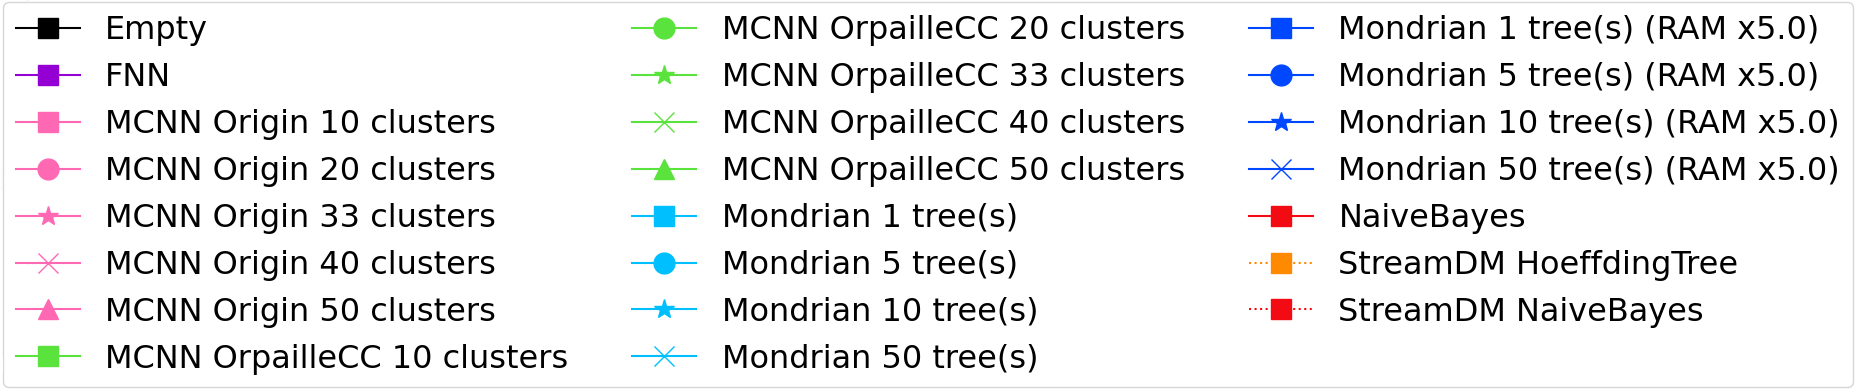
\includegraphics[width=0.8\linewidth]{figures/legend.png}
	\begin{subfigure}[t]{.49\linewidth}
		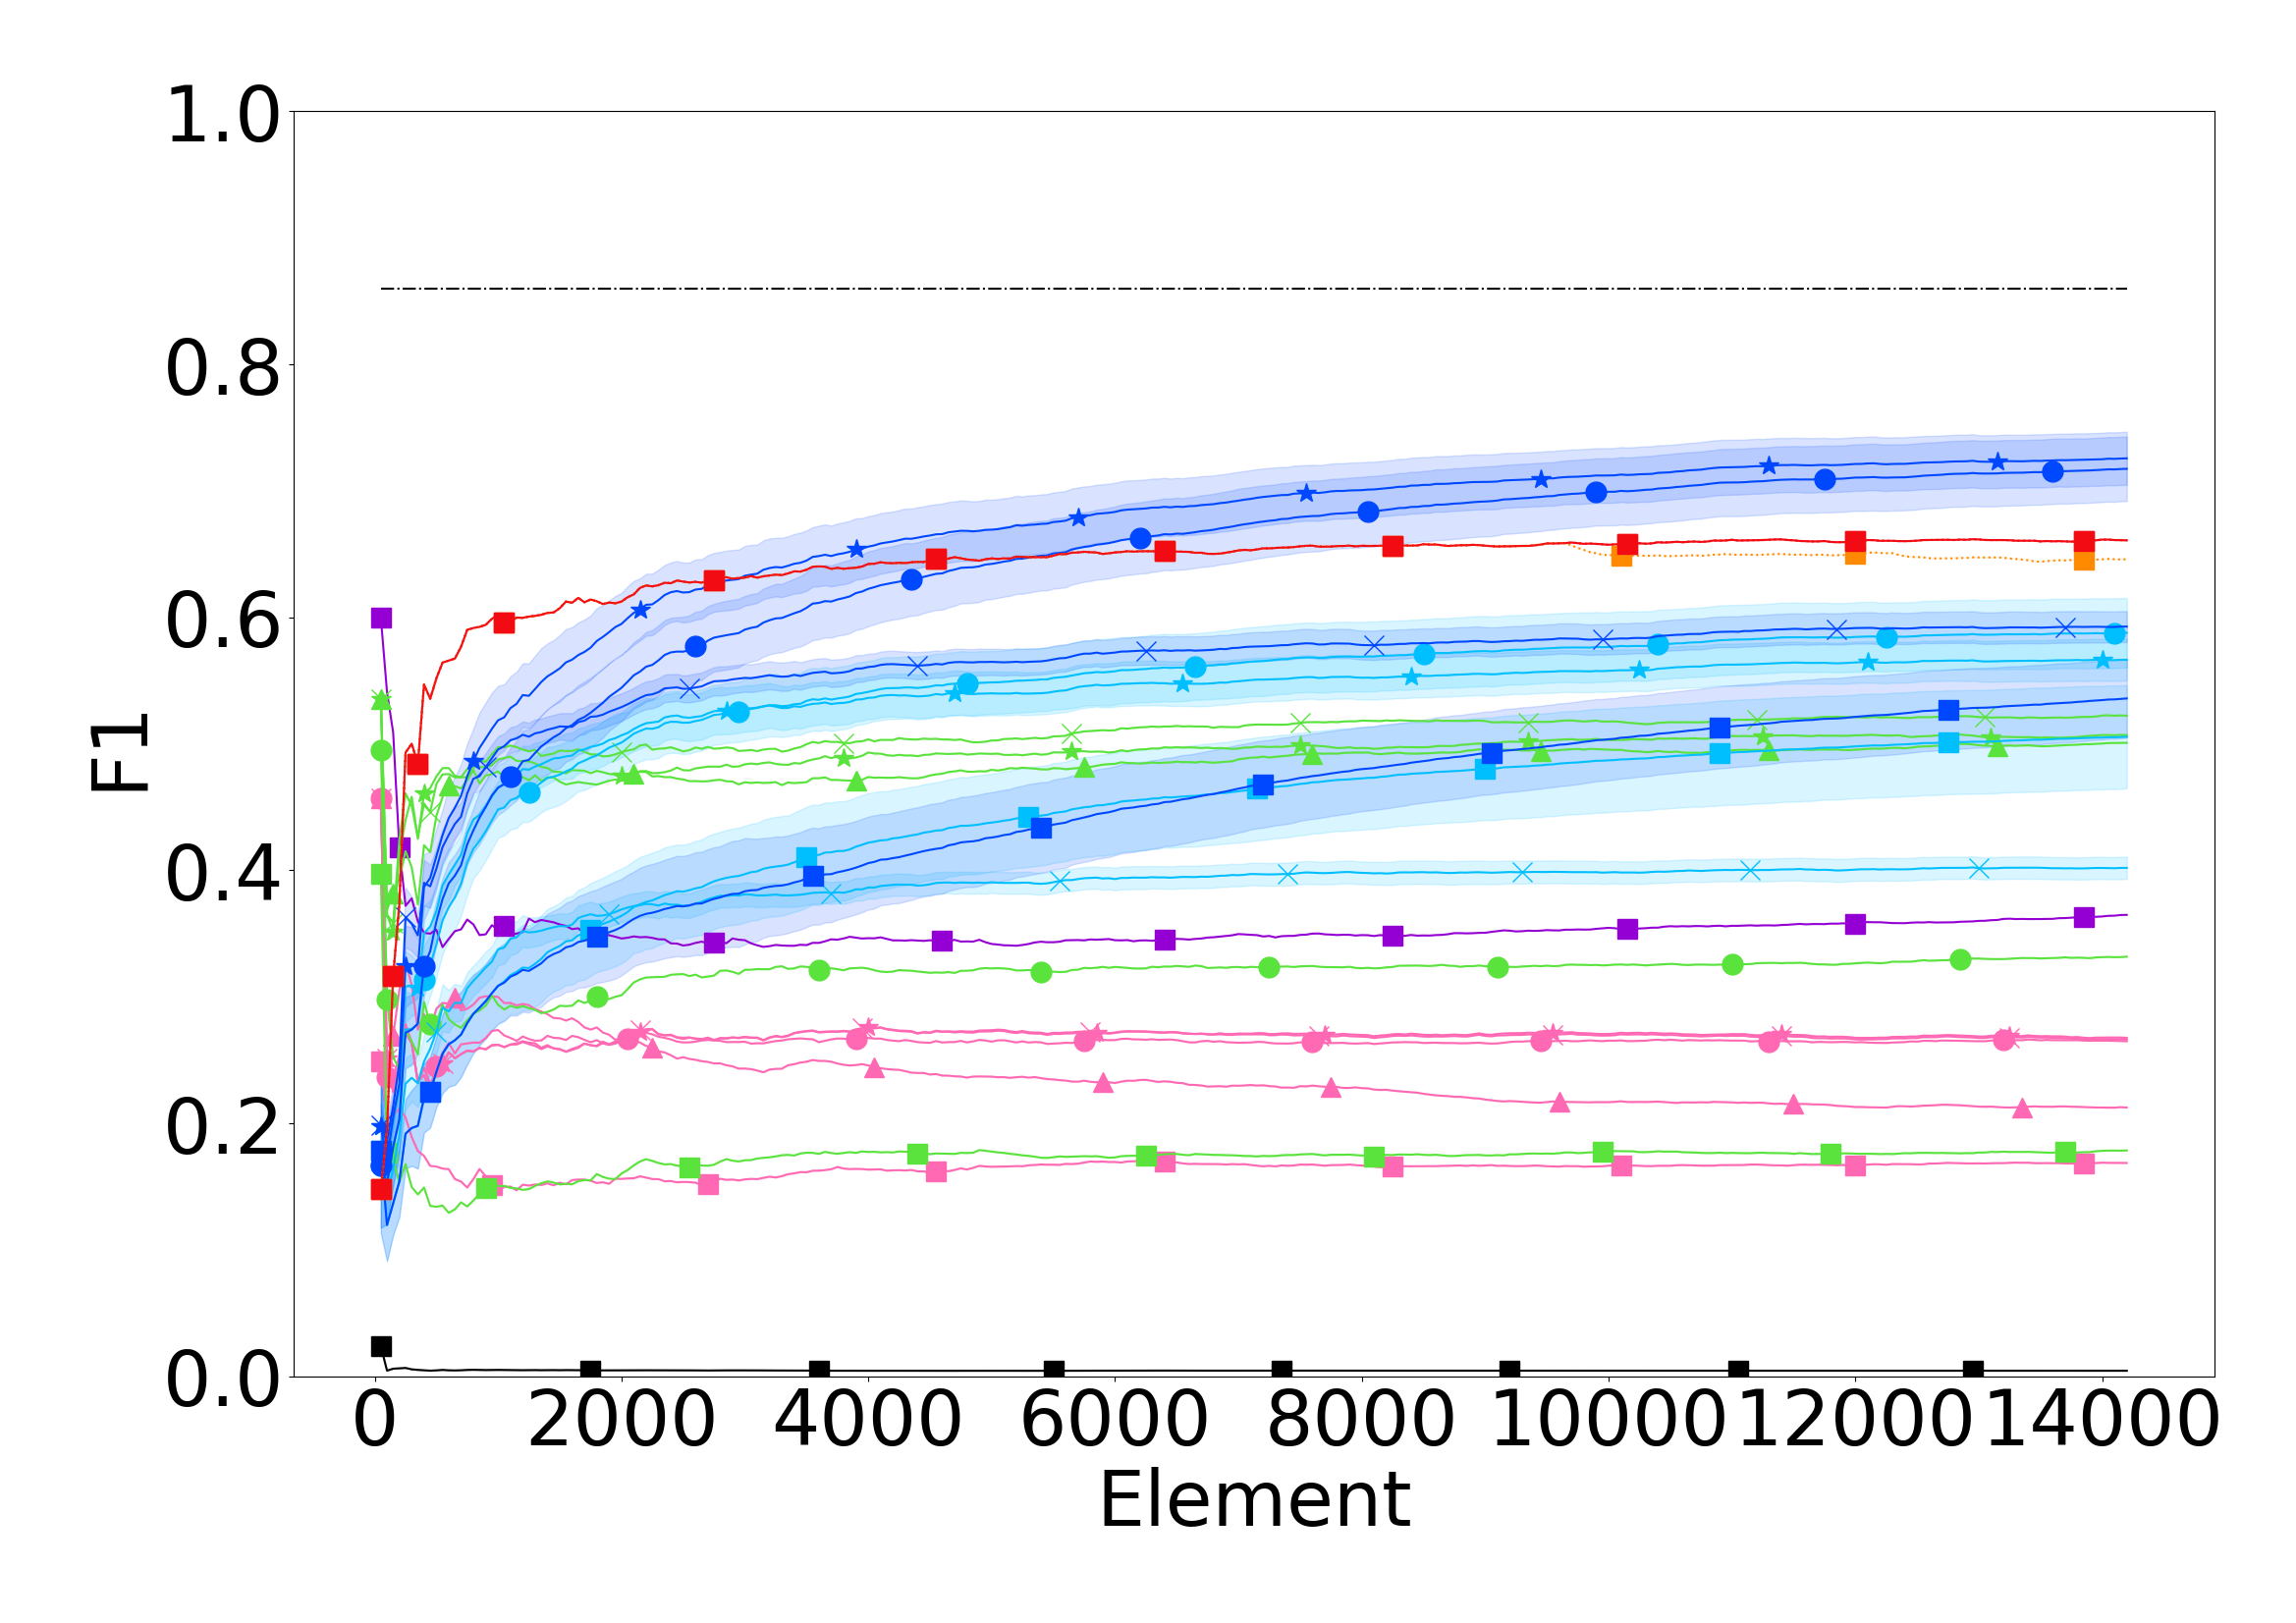
\includegraphics[width=\linewidth]{figures/results/banos_6_f1_std.png}
		\caption{\banosdataset}
		\label{fig:f1-banos}
	\end{subfigure}
	\begin{subfigure}[t]{.49\linewidth}
		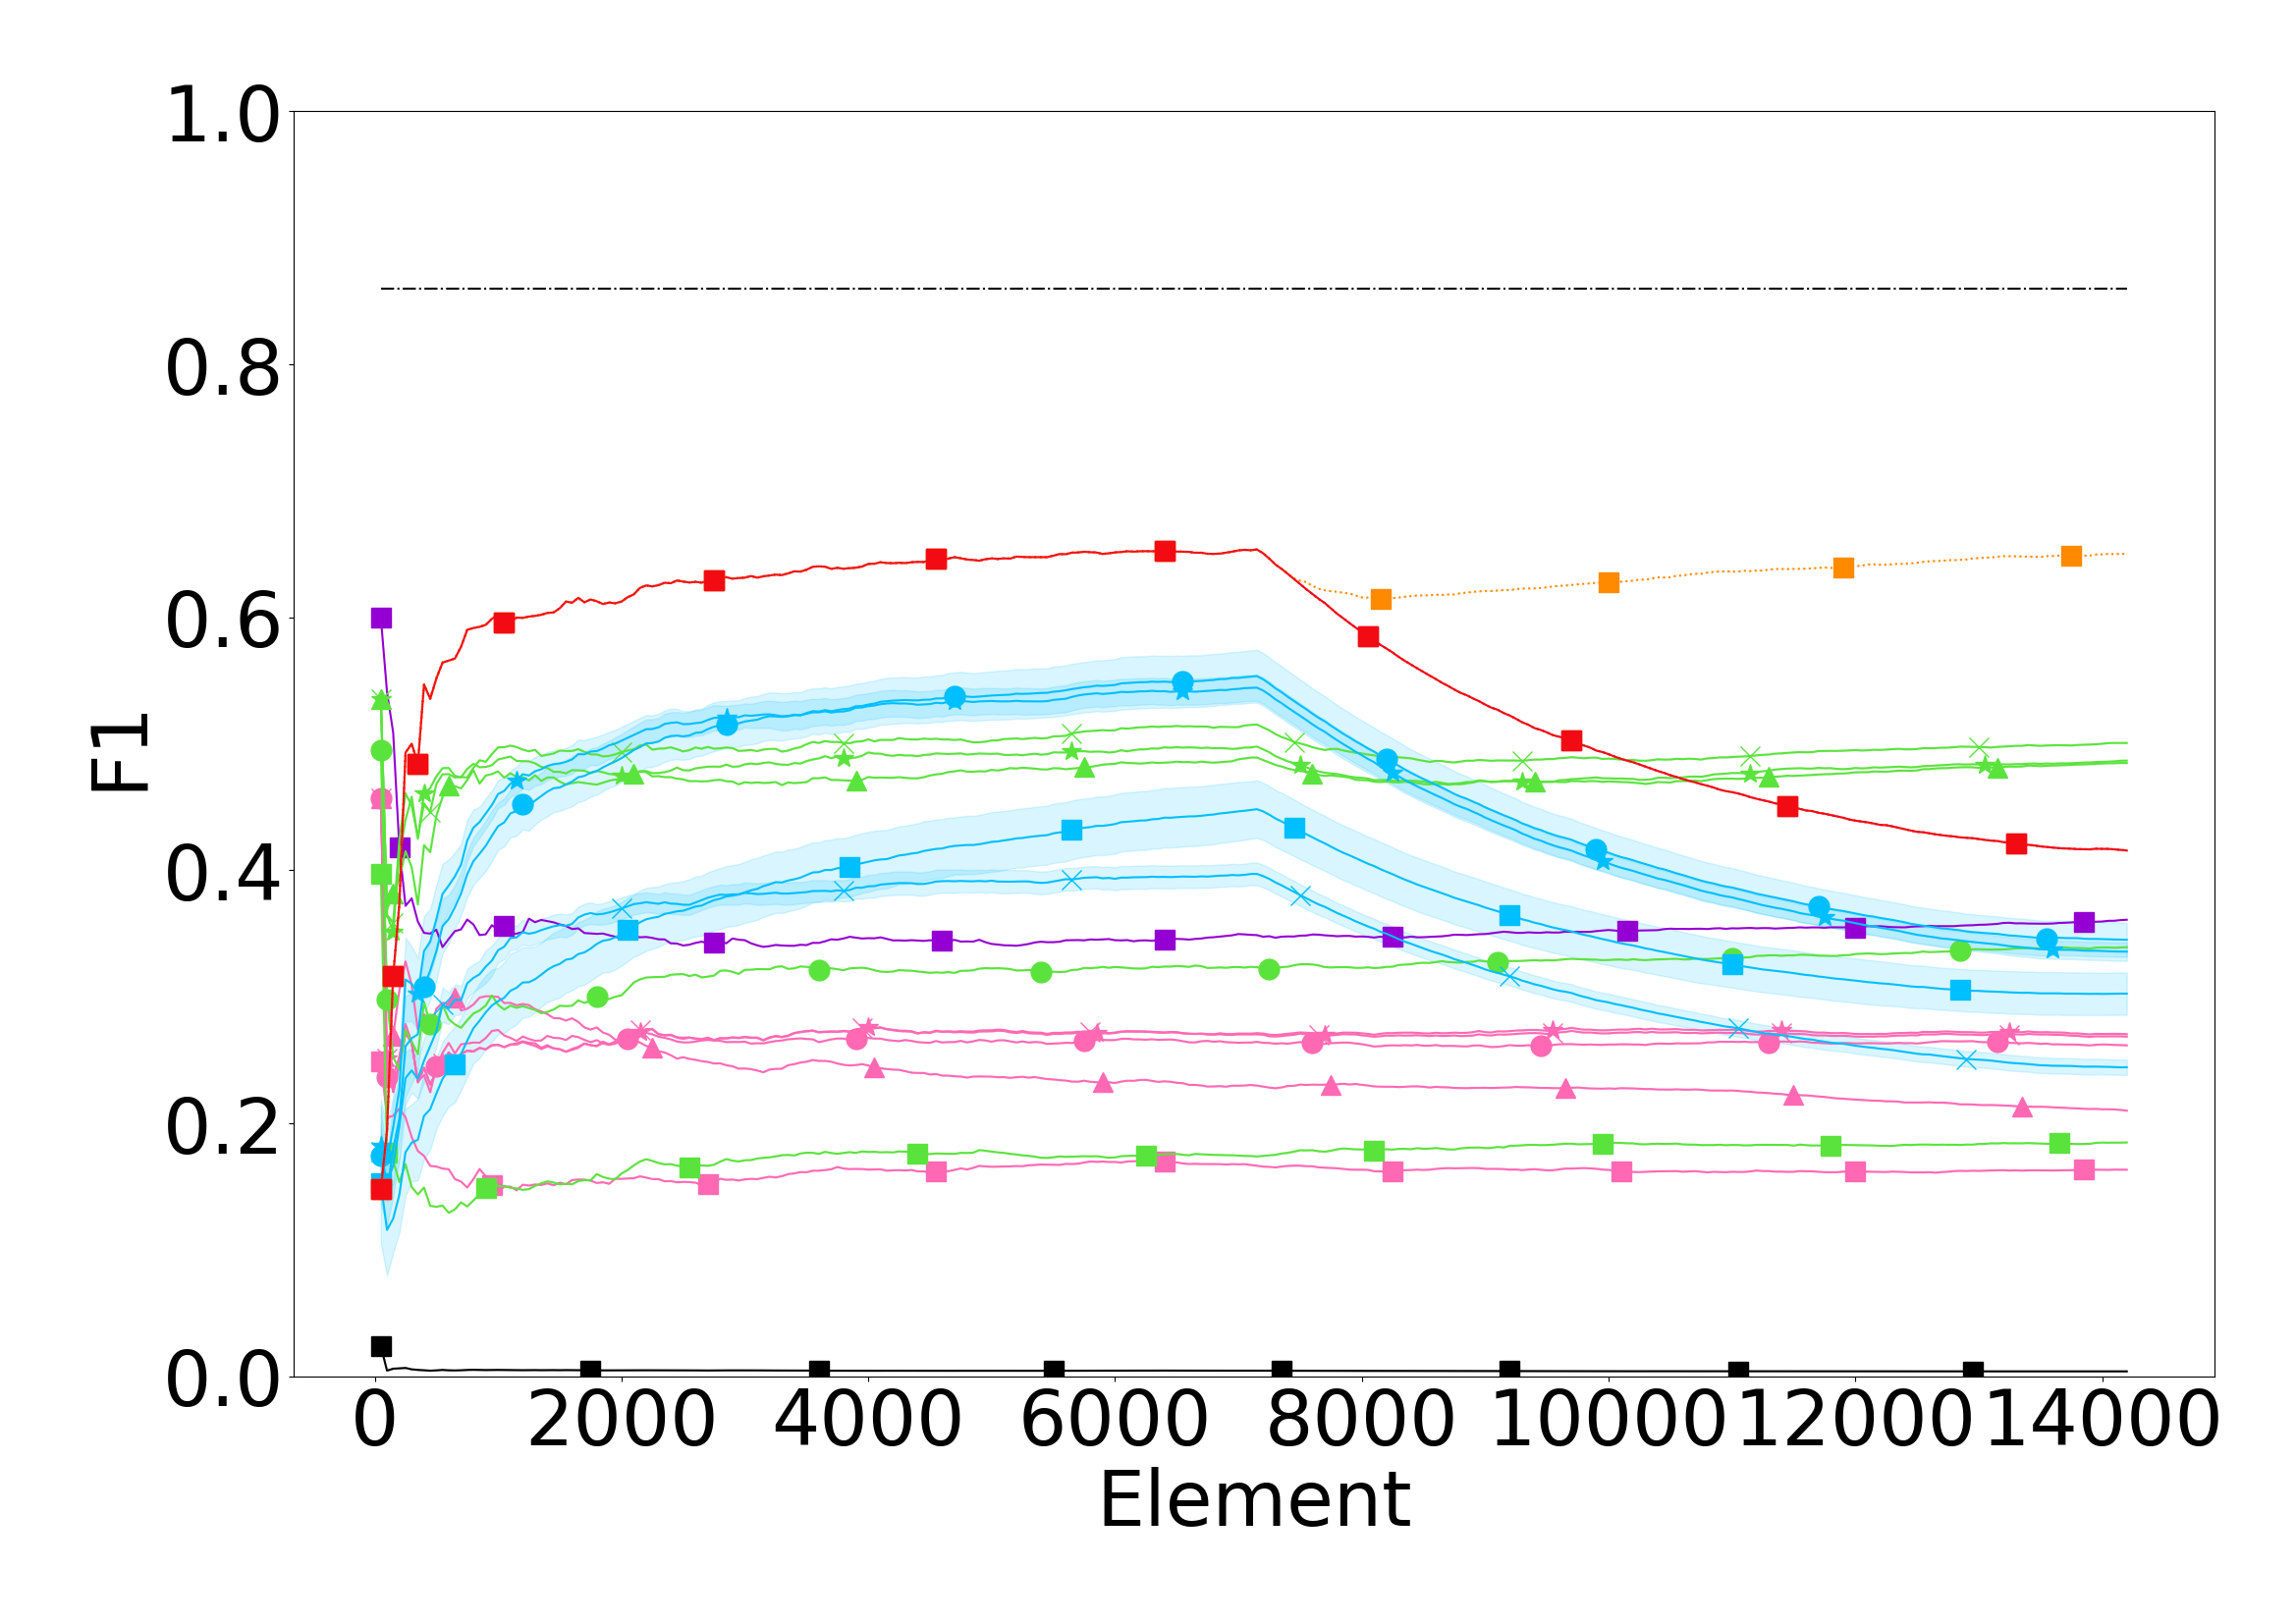
\includegraphics[width=\linewidth]{figures/results/drift_6_f1_std.png}
		\caption{\banosdataset (with Drift)}
		\label{fig:f1-drift}
	\end{subfigure}\\
	\begin{subfigure}[t]{.49\linewidth}
		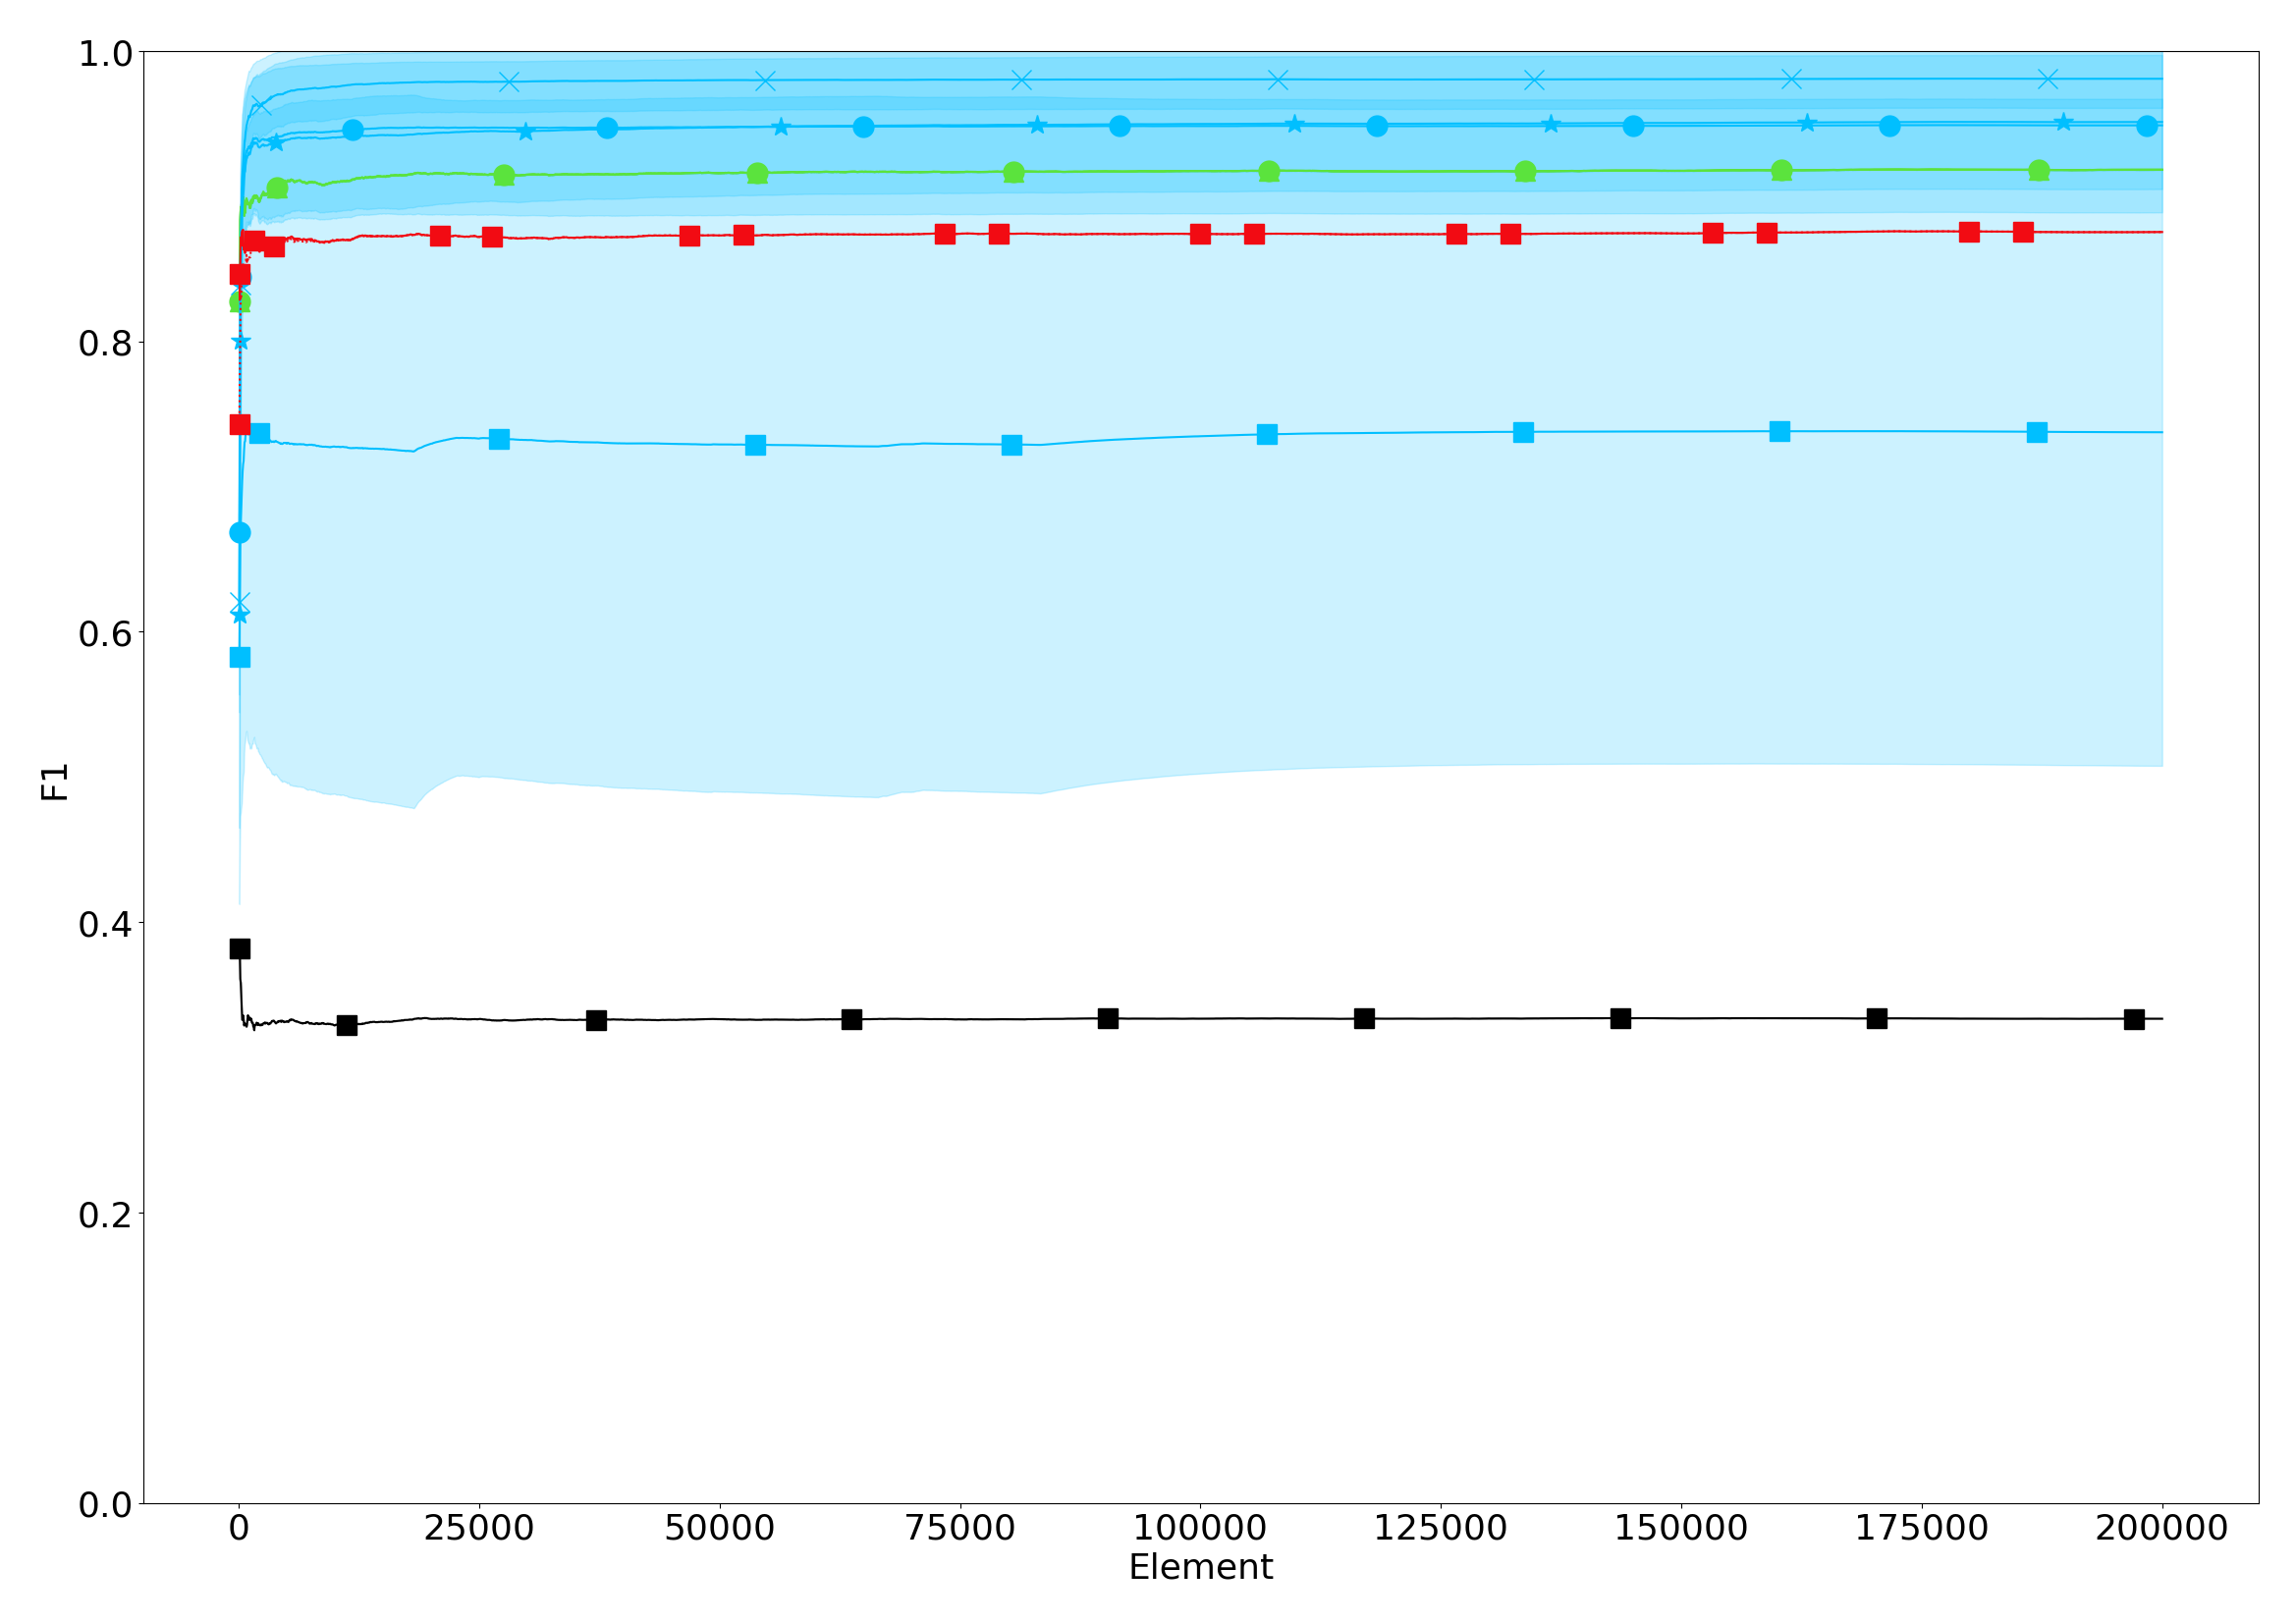
\includegraphics[width=\linewidth]{figures/results/dataset_1_f1_std.png}
		\caption{Hyperplane (MOA)}
		\label{fig:f1-dataset_1}
	\end{subfigure}
	\begin{subfigure}[t]{.49\linewidth}
		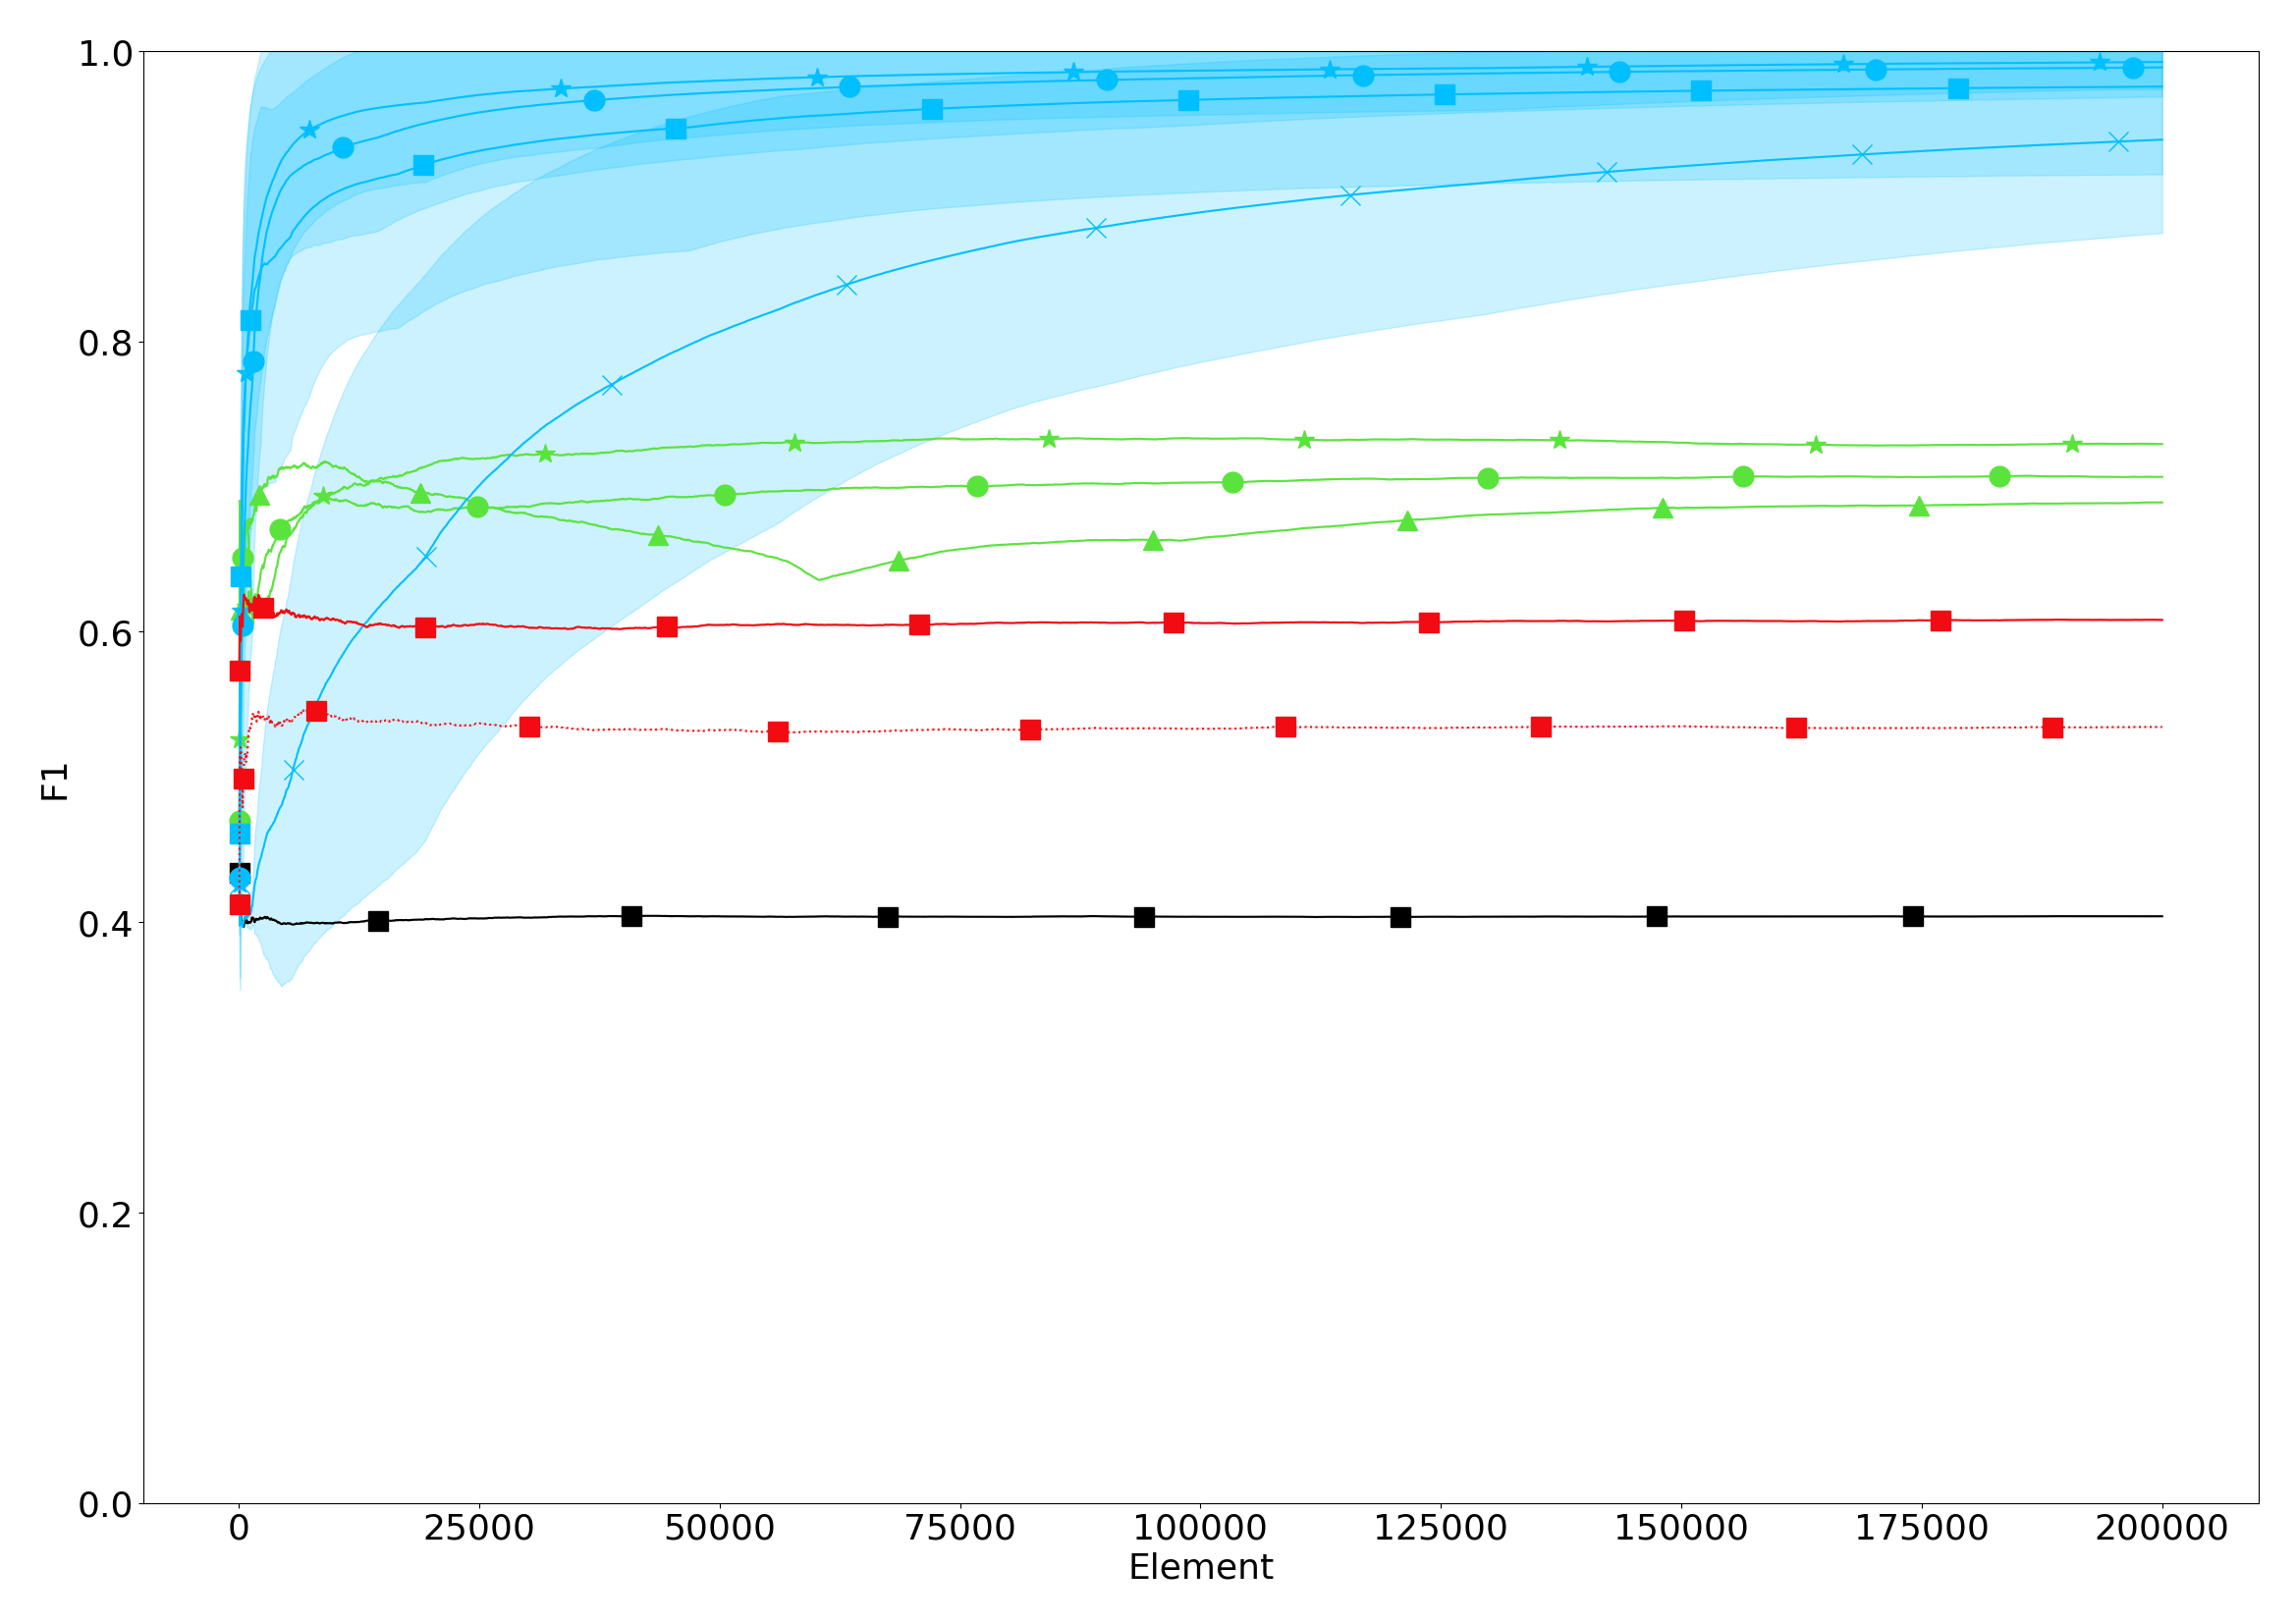
\includegraphics[width=\linewidth]{figures/results/dataset_2_f1_std.png}
		\caption{RandomRBF (MOA)}
		\label{fig:f1-dataset_2}
	\end{subfigure}\\
	\begin{subfigure}[t]{.49\linewidth}
		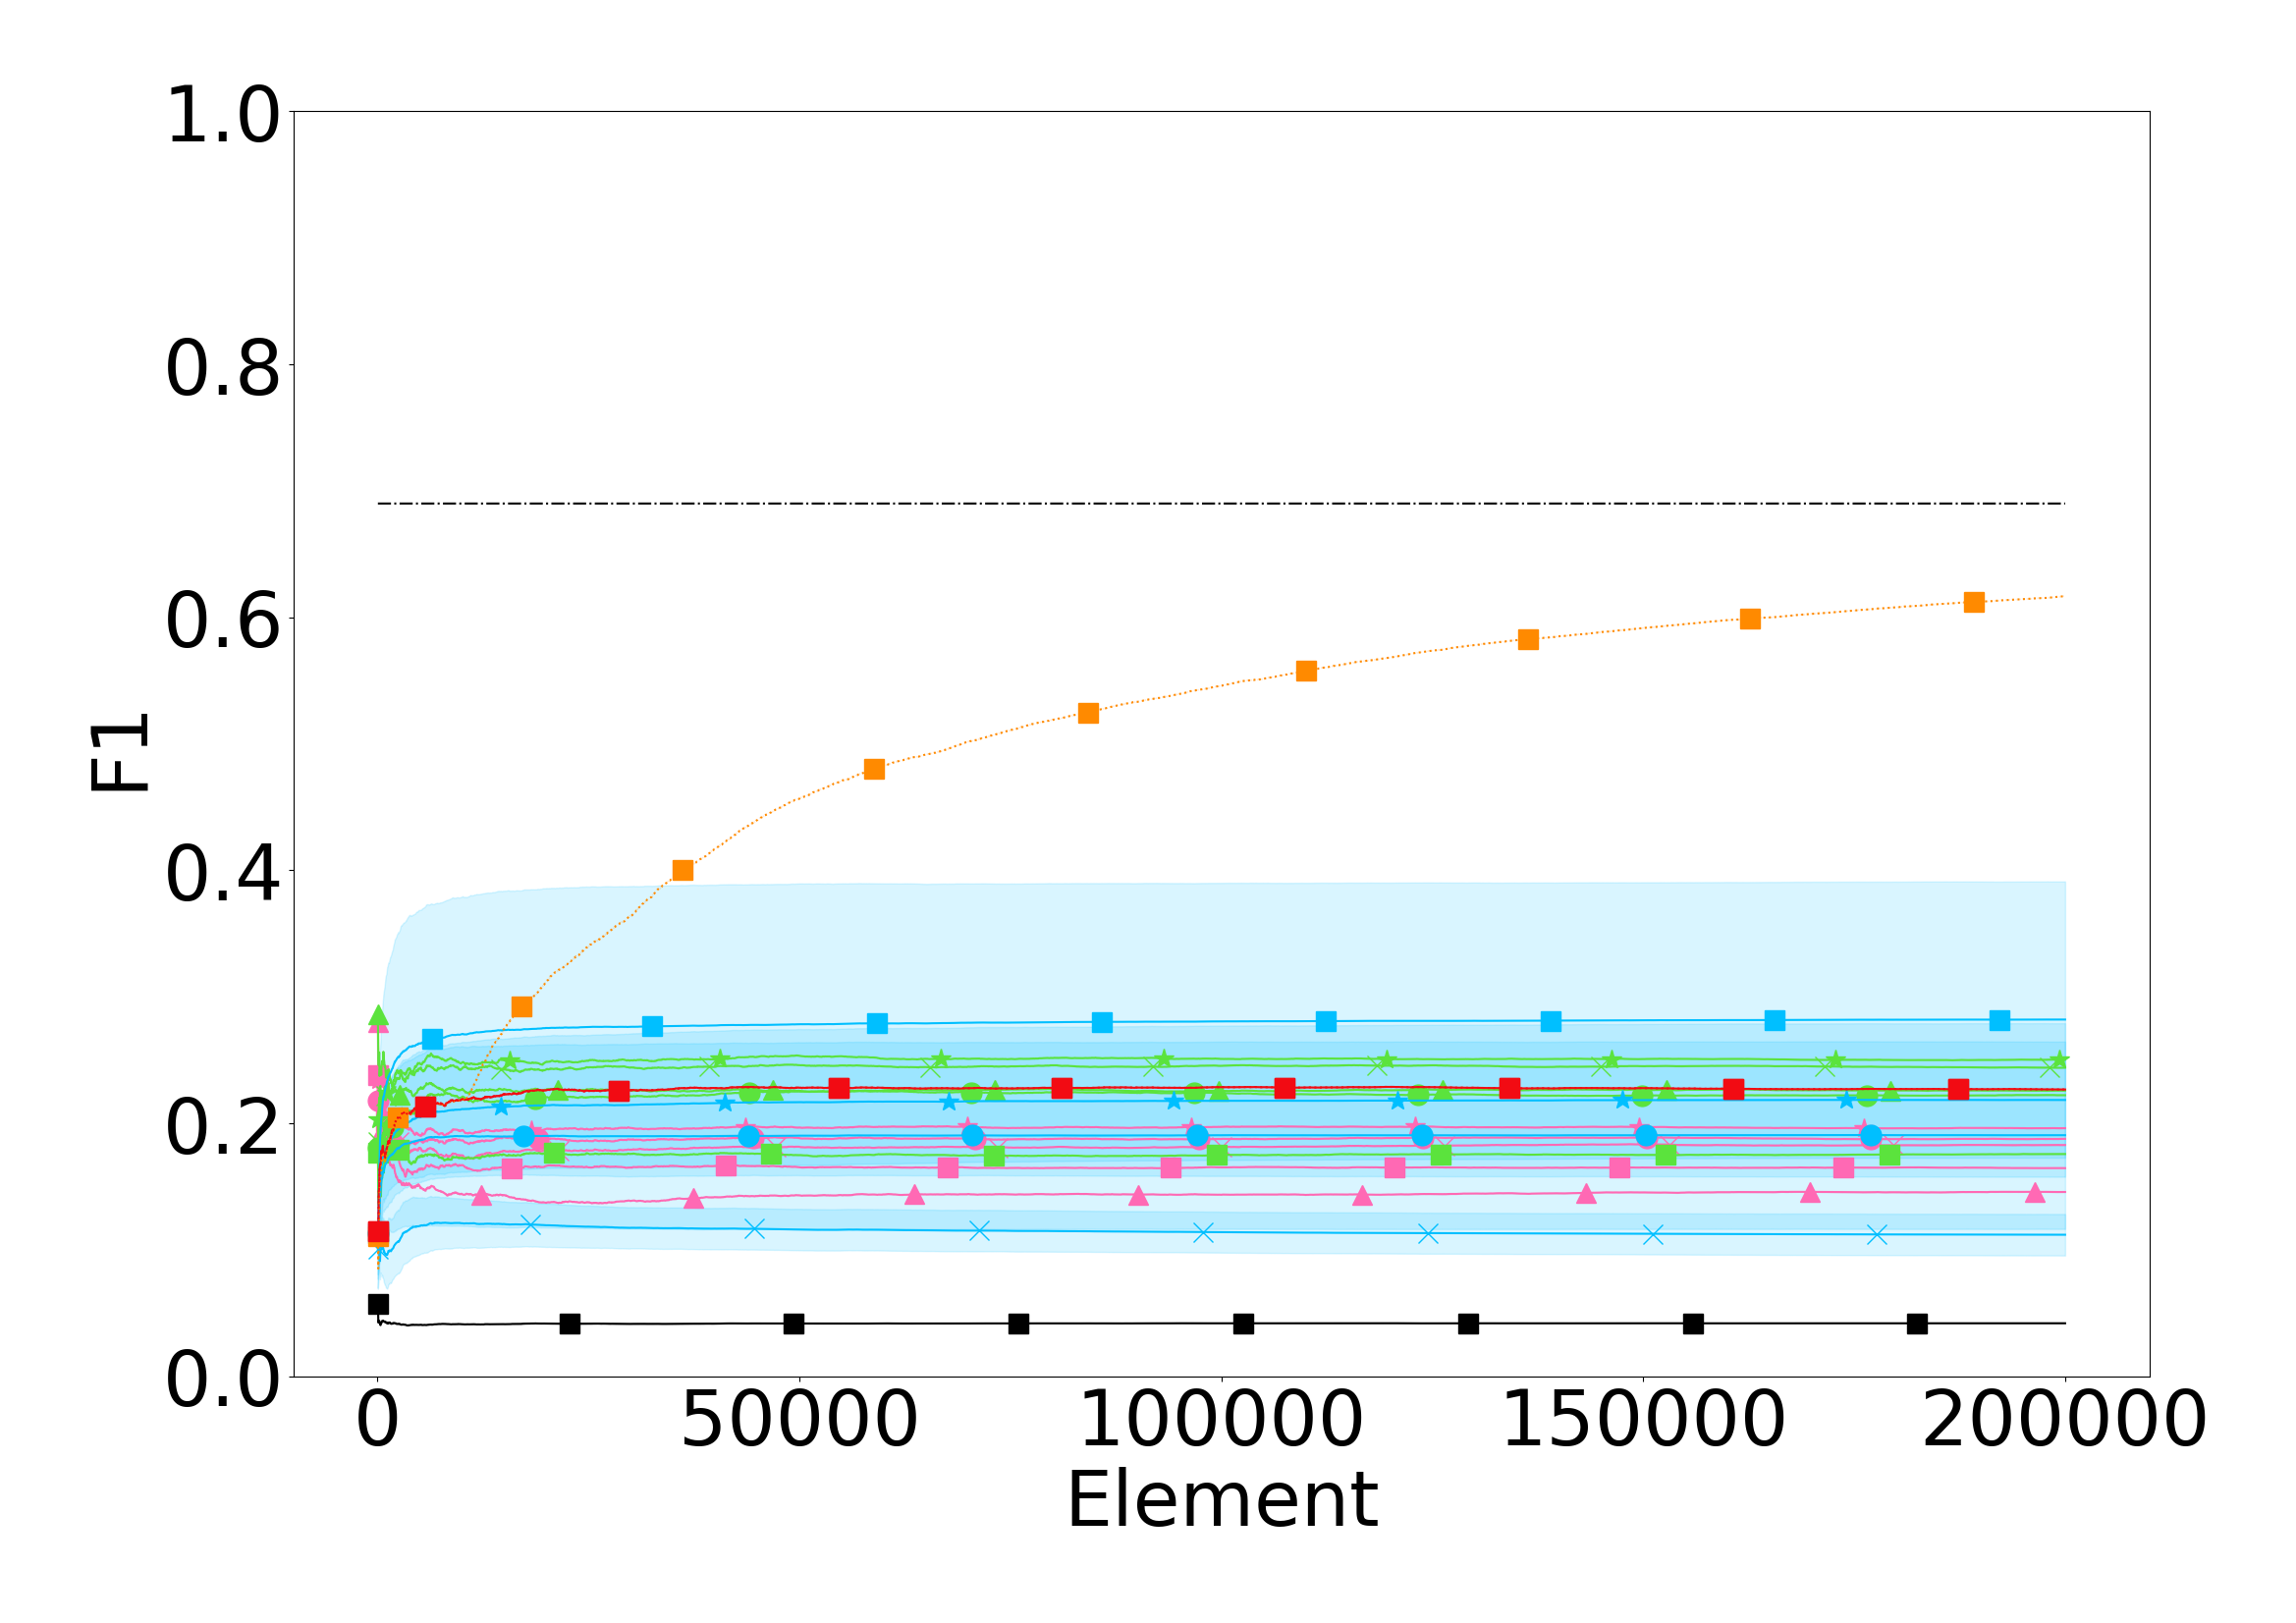
\includegraphics[width=\linewidth]{figures/results/dataset_3_f1_std.png}
		\caption{RandomTree (MOA)}
		\label{fig:f1-dataset_3}
	\end{subfigure}
	\begin{subfigure}[t]{.49\linewidth}
		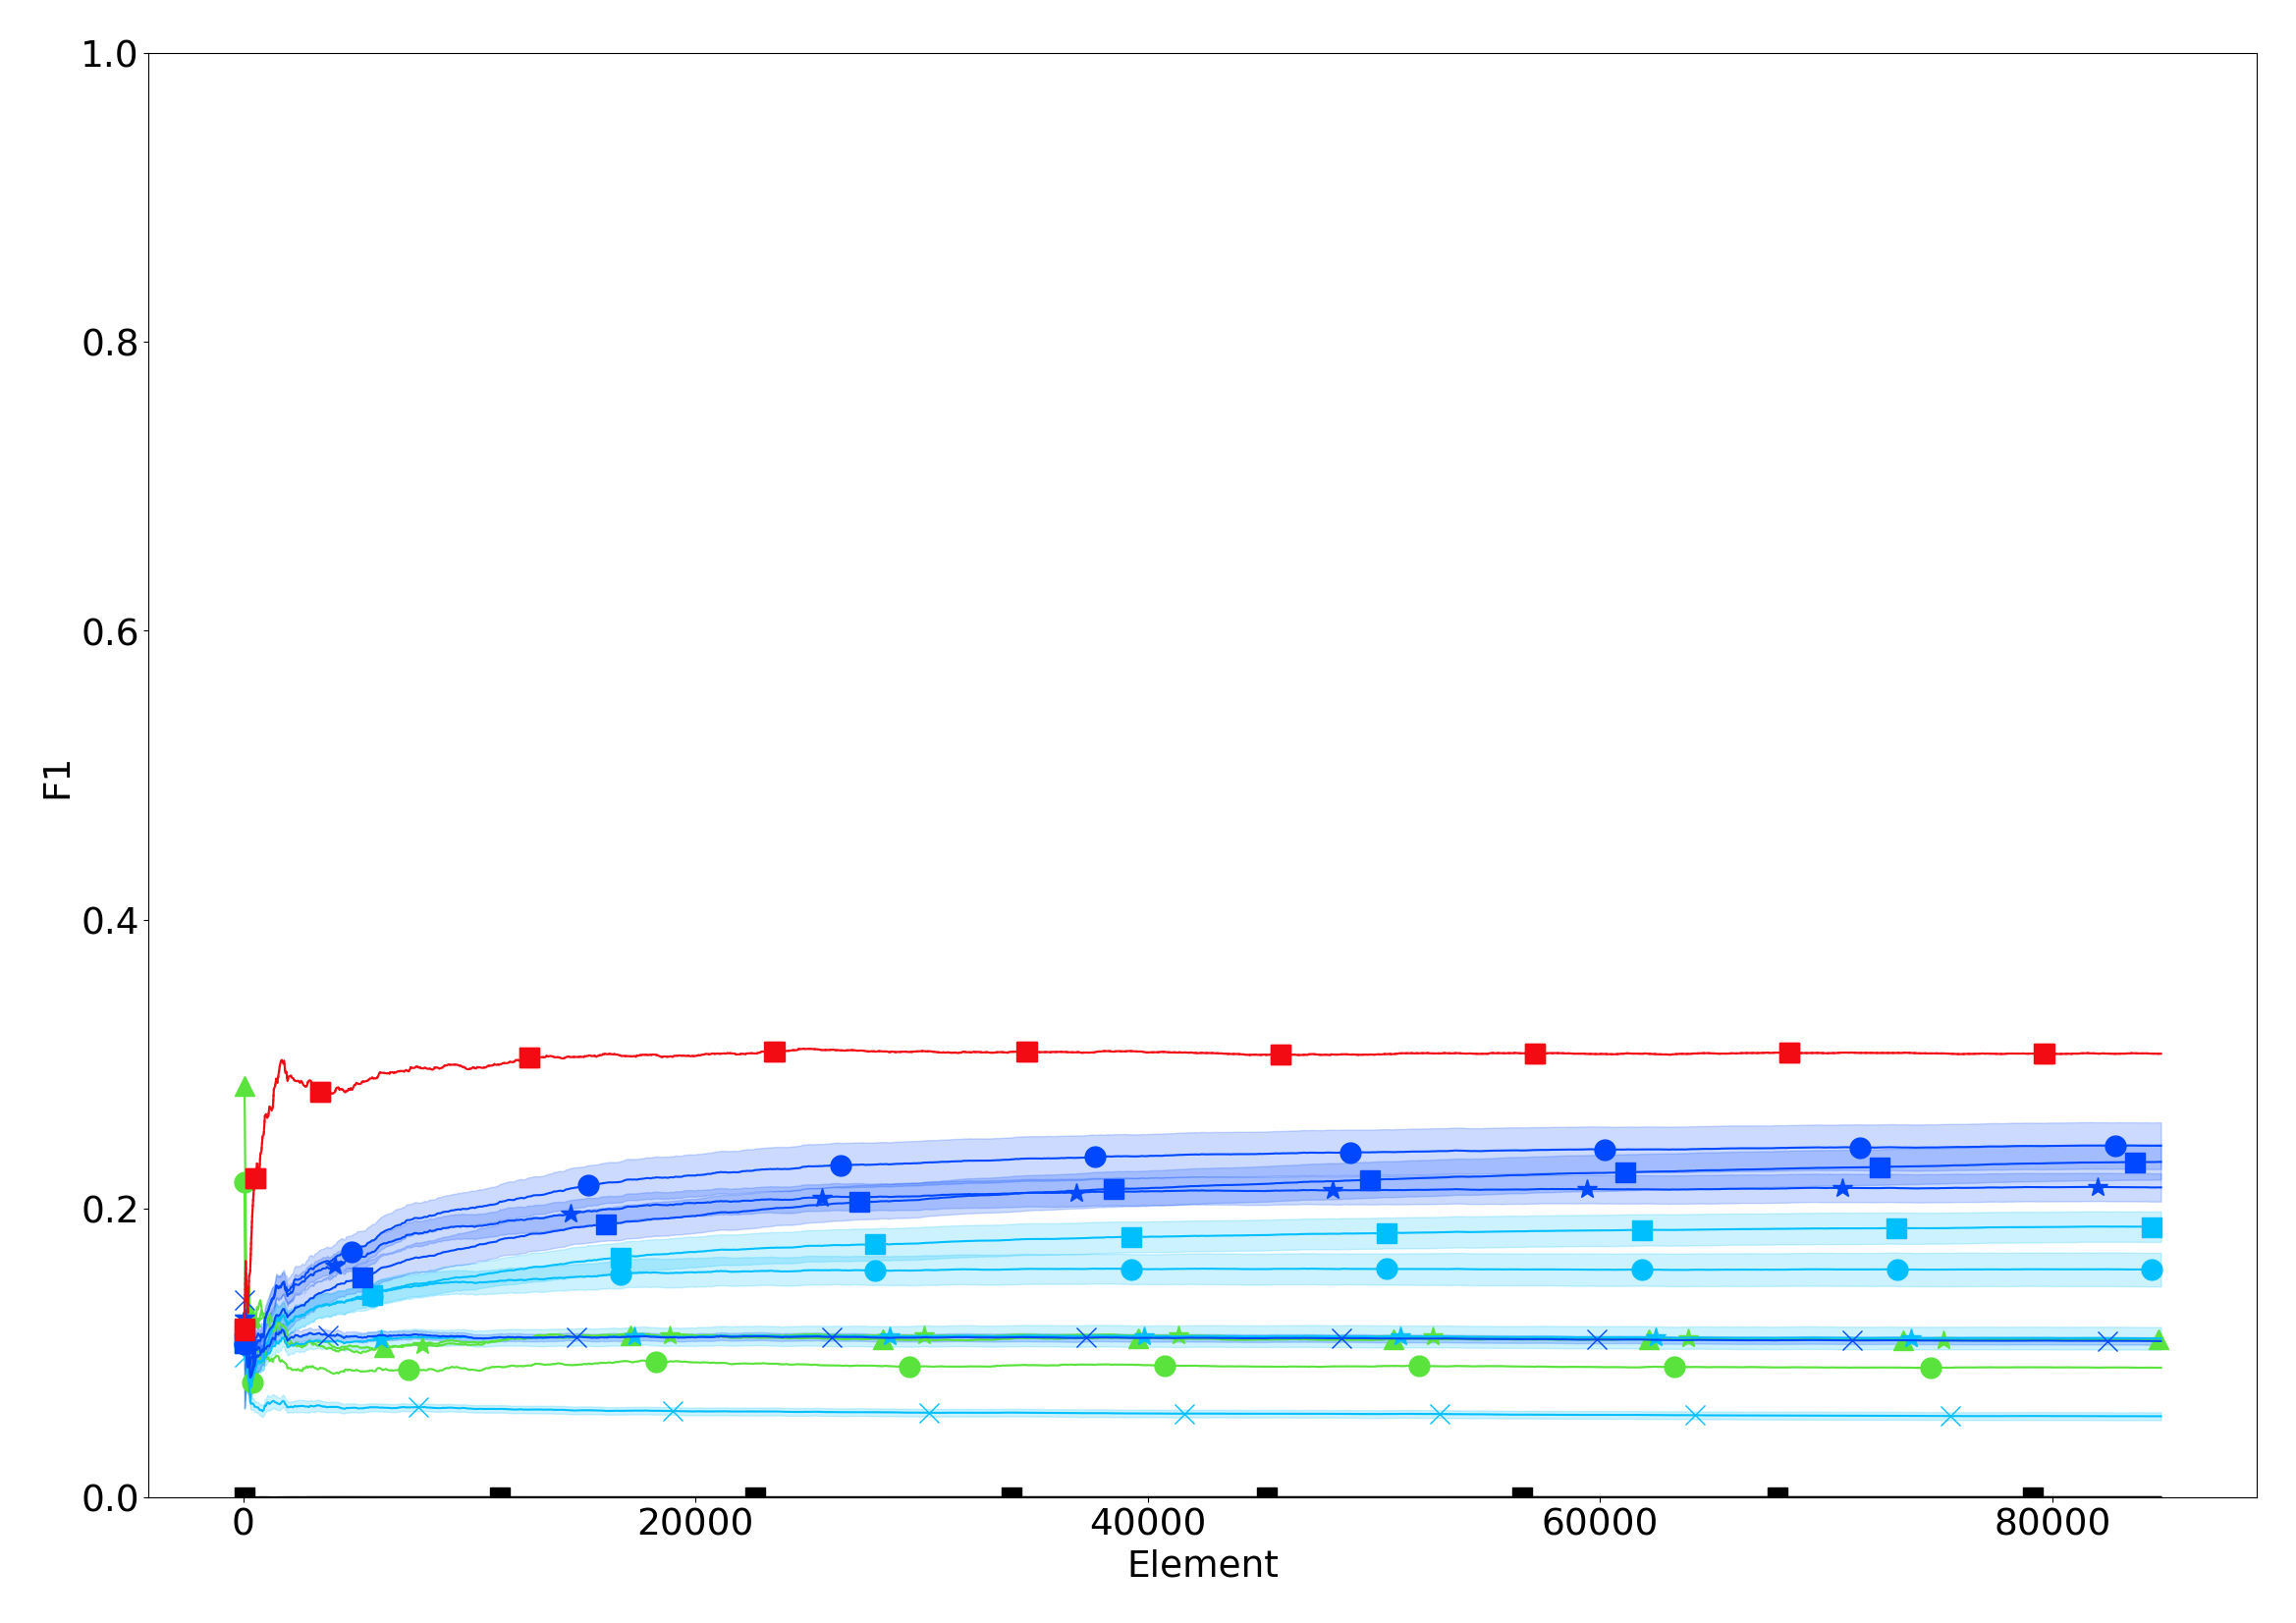
\includegraphics[width=\linewidth]{figures/results/recofit_6_f1_std.png}
		\caption{\recofitdataset}
		\label{fig:f1-recofit}
	\end{subfigure}
	\caption{F1 scores for the six datasets (average over 20 repetitions).
		The horizontal dashed black line indicates the offline \knn F1
		score (the value of k was obtained by grid search in [2, 20]). The
		blue shades represent a $\pm\sigma$ interval of the \mondrianforest
		classifier across repetitions.}
	\label{fig:f1}
\end{figure*}

\section{Results}
This section presents our benchmark results and the corresponding
hyperparameter tunning experiments.


\subsection{Overall classification performance}

%General description
Figure~\ref{fig:f1} compares the F1 scores obtained by all classifiers on
the six datasets. The graphs also show the standard deviation of the
\mondrianforest classifier observed across all repetitions (the other
classifiers do not involve any randomness). 

F1 scores vary greatly across the datasets. While the highest
observed F1 score is above 0.95 on the Hyperplane and RandomRBF datasets,
it barely reaches 0.65 for the \banosdataset dataset, and it remains under
0.40 on the \recofitdataset and RandomTree datasets. This trend is
consistent for all classifiers.

%Offline observations
The offline \knn classifier used as baseline achieves better F1 scores than
all other classifiers, except for the \mondrianforest on the Hyperplane and
the RandomRBF datasets. On the \banosdataset dataset, the difference of
\TG{x} with the best stream classifier remains very substantial, which
quantifies the remaining performance gap between data stream and offline
classifiers. On the \recofitdataset dataset, the difference between stream
and offline classifiers is lower, but the offline performance remains very
low.
%Recofit 9
%Banos 3
%Hyperplane 19
%RandomRBF 19
%RandomTree 15
%Drift 11

It should be noted that the F1 scores observed for the offline \knn
classifier on the real datasets are substantially lower than the values
reported in the literature. On the \banosdataset dataset, the original
study in~\cite{Banos_2014} reports an F1 score of 0.96, the work
in~\cite{behzad2019} achieves 0.92, but our benchmark only achieves 0.86.
Similarly, on the \recofitdataset dataset, \TG{check original study} the
work in~\cite{behzad2019} reaches 0.65 while our benchmark only achieves
0.40. This is most likely due to our use of data coming from a single
sensor, consistently with our motivating use case, while the other works used mutiple ones (\TG{x} in the case of
\banosdataset, \TG{y} in the case of \recofitdataset).

% %One sensor
% In this study, we focused on using one sensor rather than all the sensors
% available in the real datasets. In the case of more sensor used, we would expect
% an F1 score improvement for all classifiers because they would have access to
% more data in order to discriminate the classes. 
% On the other hand, we would
% expect an increase in the memory footprint because more sensors mean more
% attribute extracted. 
% This should have minimal impact on classifiers such as
% \naivebayes because their footprint is already low. However, the
% \mondrianforest, the \hoeffdingtree, and \mcnn memory footprints are expected to
% grow significatively because more sensors means more attributes for each leaf or
% cluster. In particular, we expect the \mondrianforest F1 score to be mitigated
% by the decrease of memory induced by the increased leave size \TG{Merge in second paragraph of sub-section A.}.

%Concept drift
The \hoeffdingtree appears to be the most robust to concept drifts
(\banosdataset (with drift)), while the \mondrianforest and \naivebayes
classifiers are the most impacted. \mcnn classifiers are marginally impacted.
The low resilience of \mondrianforest to concept drifts can be attributed to
two factors. First, existing nodes in trees of a \mondrianforest cannot be updated.
Second, when the memory limit is reached, \mondriantrees cannot grow
or reshape their structure anymore.


\subsection{\hoeffdingtree and \naivebayes}

%Hoeffding and Naïve Bayes description when they are the best
The \naivebayes and the \hoeffdingtree classifiers stand out on the two real datasets
(\banosdataset and \recofitdataset) even though the F1 scores observed remain
low (0.6 and 0.35) compared to offline \knn (0.86 and 0.40). Additionally, the
\hoeffdingtree performs outstandingly on the RandomTree dataset and
\banosdataset dataset with a drift. Such good performances where expected on the
RandomTree dataset because it was generated based on a tree structure, however

%Explanation of their F1 score similarity
Except for the \banosdataset dataset, the \hoeffdingtree performs better
than \naivebayes. For all datasets, the performance of both classifiers is
comparable at the beginning of the stream, because the \hoeffdingtree uses
a \naivebayes in its leaves.  However, F1 scores diverge throughout the
stream, most likely because of the \hoeffdingtree's ability to reshape its
tree structure.  This occurs after a sufficient amount of elements, and the
difference is more noticeable after a concept drift.

%Naive Bayes and Naive Bayes
Finally, we note that the StreamDM and OrpailleCC implementations of
\naivebayes are indistinguishable from each other, which confirms our
implementation in OrpailleCC.

\subsection{\mondrianforest}

%Mondrian when at best
On two synthetic datasets, Hyperplane and RandomRBF, the \mondrianforest (RAM x
1.0) with 10 trees achieves the best performance (F1$>$0.95), above the offline
\knn.  Additionally, the \mondrianforest with 5 or 10 trees ranks third on the
two real datasets. 

%Mondrian discussion
Surprisingly, a \mondrianforest with 50 trees performs worse than 5 or 10
trees on most datasets. The only exception is the Hyperplane dataset where
50 trees perform between 5 and 10 trees. This is due to the fact that
our \mondrianforest implementation is memory bounded, which is
useful on connected objects but limits tree growth when the allocated memory is
full. Because 50 trees fill the memory faster than 10 or 5 trees, the
learning stops earlier, before the trees can learn learned enough from the
data. It can also be noted that the variance of the F1 score decreases with
the number of trees, as expected.

%Mondrian RAMx5
This dependency of the \mondrianforest to memory allocation is shown in
\banosdataset and \recofitdataset datasets, where an additional
configuration with five times more memory than the initial configuration is
shown (total of 3~MB).  The memory increase induces an F1 score difference
greater than 0.1, except when only one tree is used, in
which case the improvement caused by the memory is less than 0.05. Note that the
selected memory bound may not be achievable on a connected object. Overall,
\mondrianforest seems to be a viable alternative to \naivebayes or the
\hoeffdingtree for \har.


\subsection{\mcnn}

%MCNN observations
The \mcnn OrpailleCC stands out on \banosdataset (with drift) dataset where it
ranks second thanks to its adaptation to the concept drift.  On other datasets,
\mcnn OrpailleCC ranks below the \mondrianforest and the \hoeffdingtree, but
above \mcnn Original. This difference between the two \mcnns is presumably due
to the fact that \mcnn Origin removes clusters with low participation too early.
On the real datasets (\banosdataset and \recofitdataset), we notice that the
\mcnn OrpailleCC appears to be learning faster than the \mondrianforest,
although the \mondrianforest catches up after a few thousand elements. Finally,
we note that \mcnn remains quite lower than the offline \knn.

\subsection{\FNN}

%FNN observation
Figure~\ref{fig:f1-banos} shows that the \FNN has a low F1 score (0.36)
compared to other classifiers (above 0.5), which contradicts the results
reported in~\cite{omid_2019} where the \FNN achieves more than 95\%
accuracy in a context of offline training. The main difference
between~\cite{omid_2019} and our study lies in the definition of the
training set. In~\cite{omid_2019}, the training set includes examples from
every subject, while we only use a single one, to ensure an objective
comparison with the other stream classifiers that do not require offline
training (except for hyperparameter tuning, done on the first subject of
the \banosdataset dataset). When we use a random sample of 10\% of the
datapoints across all subjects for offline training, we reach an F1 score
of 0.62 \TG{check value}, which is closer to the performance of the
\naivebayes classifier.

%FNN discussion
%As explained in Section~\ref{sec:method-fnn}, the pre-training of the \FNN is
%slightly different other classifiers. Indeed, the hyperparameters tuning of the
%other classifiers implies that they start the testing phase with no prior
%knowledge of the dataset, even about the element seen in the tuning phase. On
%the other hand, the \FNN starts with its weights already set from the training
%phase, therefore it has already seen datapoints from the first subject. This
%procedure genuinely helps the \FNN, otherwise the random weights would force the
%F1 score down, closer to the empty classifier.  Additionally to the
%pre-training, we used feature extraction from~\cite{omid_2019} which exhibits
%high classification performance.  Since we only trained the \FNN on the first
%subject of \banosdataset dataset, we could not apply the same neural network
%structure on other datasets.

\begin{figure*}
	\begin{subfigure}[t]{.49\linewidth}
		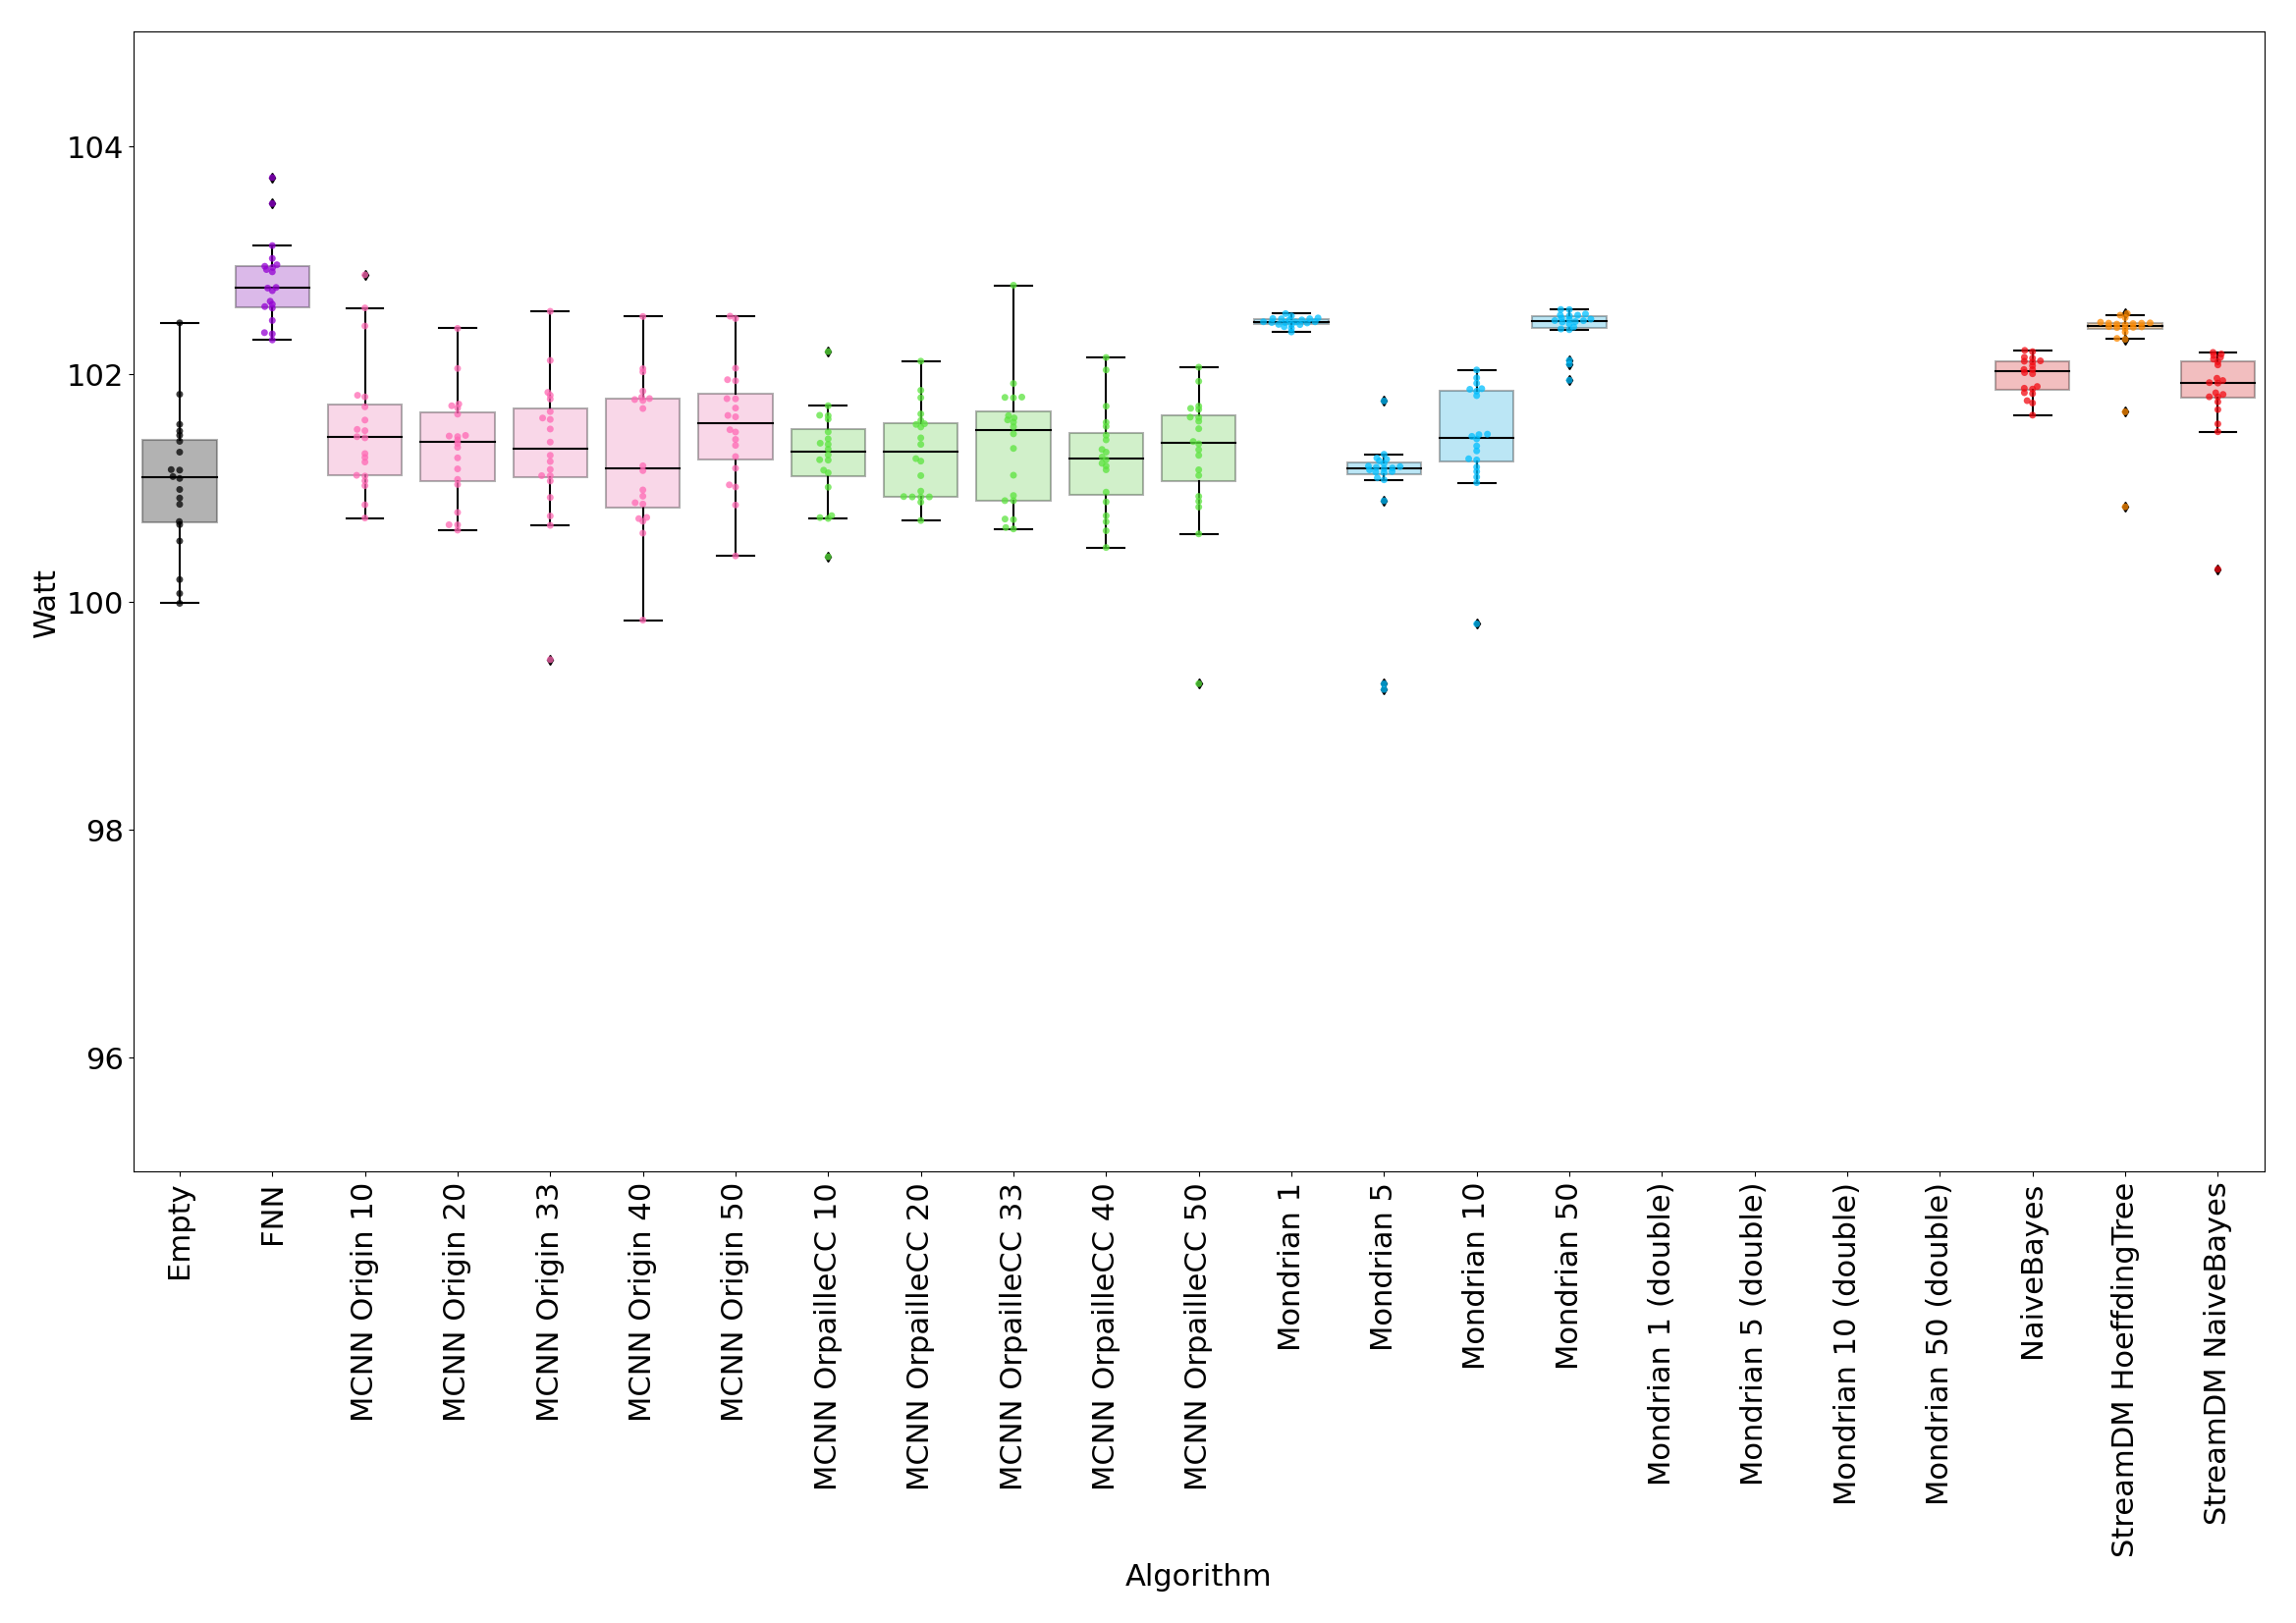
\includegraphics[width=\linewidth]{figures/results/banos_3_watt.png}
		\caption{\banosdataset}
		\label{fig:power-banos}
	\end{subfigure}
	\hfill
	\begin{subfigure}[t]{.49\linewidth}
		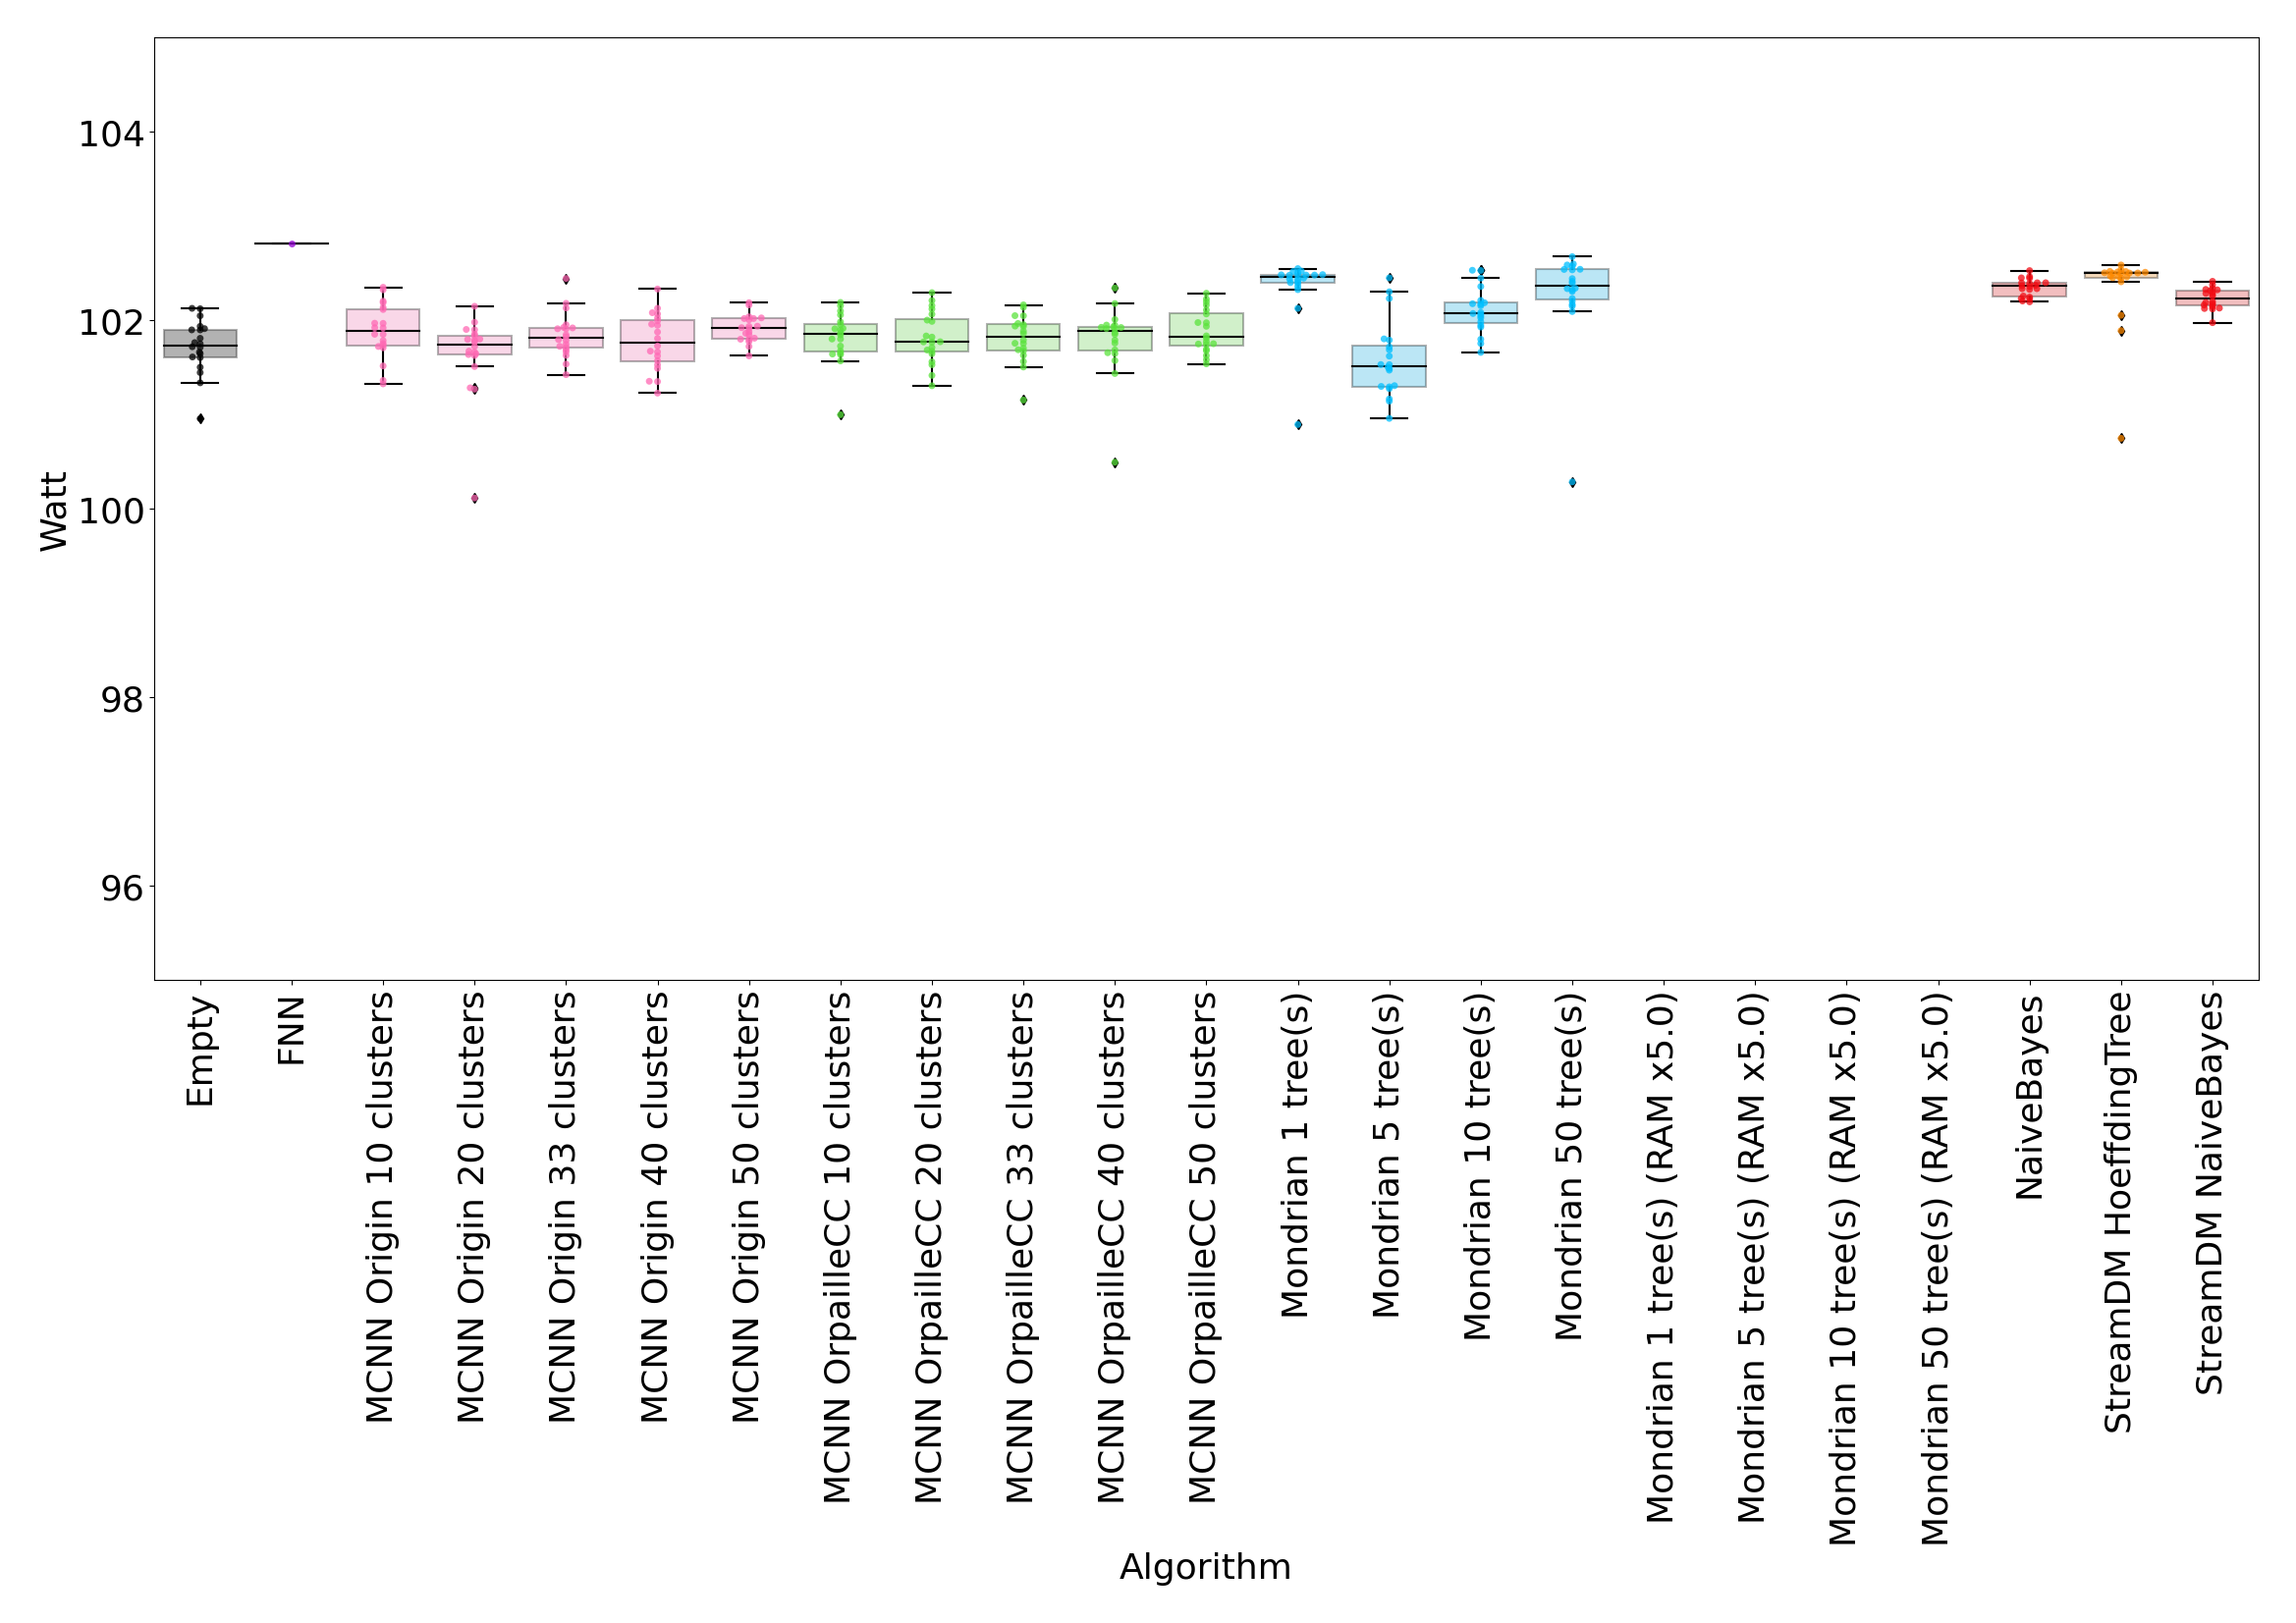
\includegraphics[width=\linewidth]{figures/results/drift_6_watt.png}
		\caption{\banosdataset with drift.}
		\label{fig:power-drift}
	\end{subfigure}\\
	\begin{subfigure}[t]{.49\linewidth}
		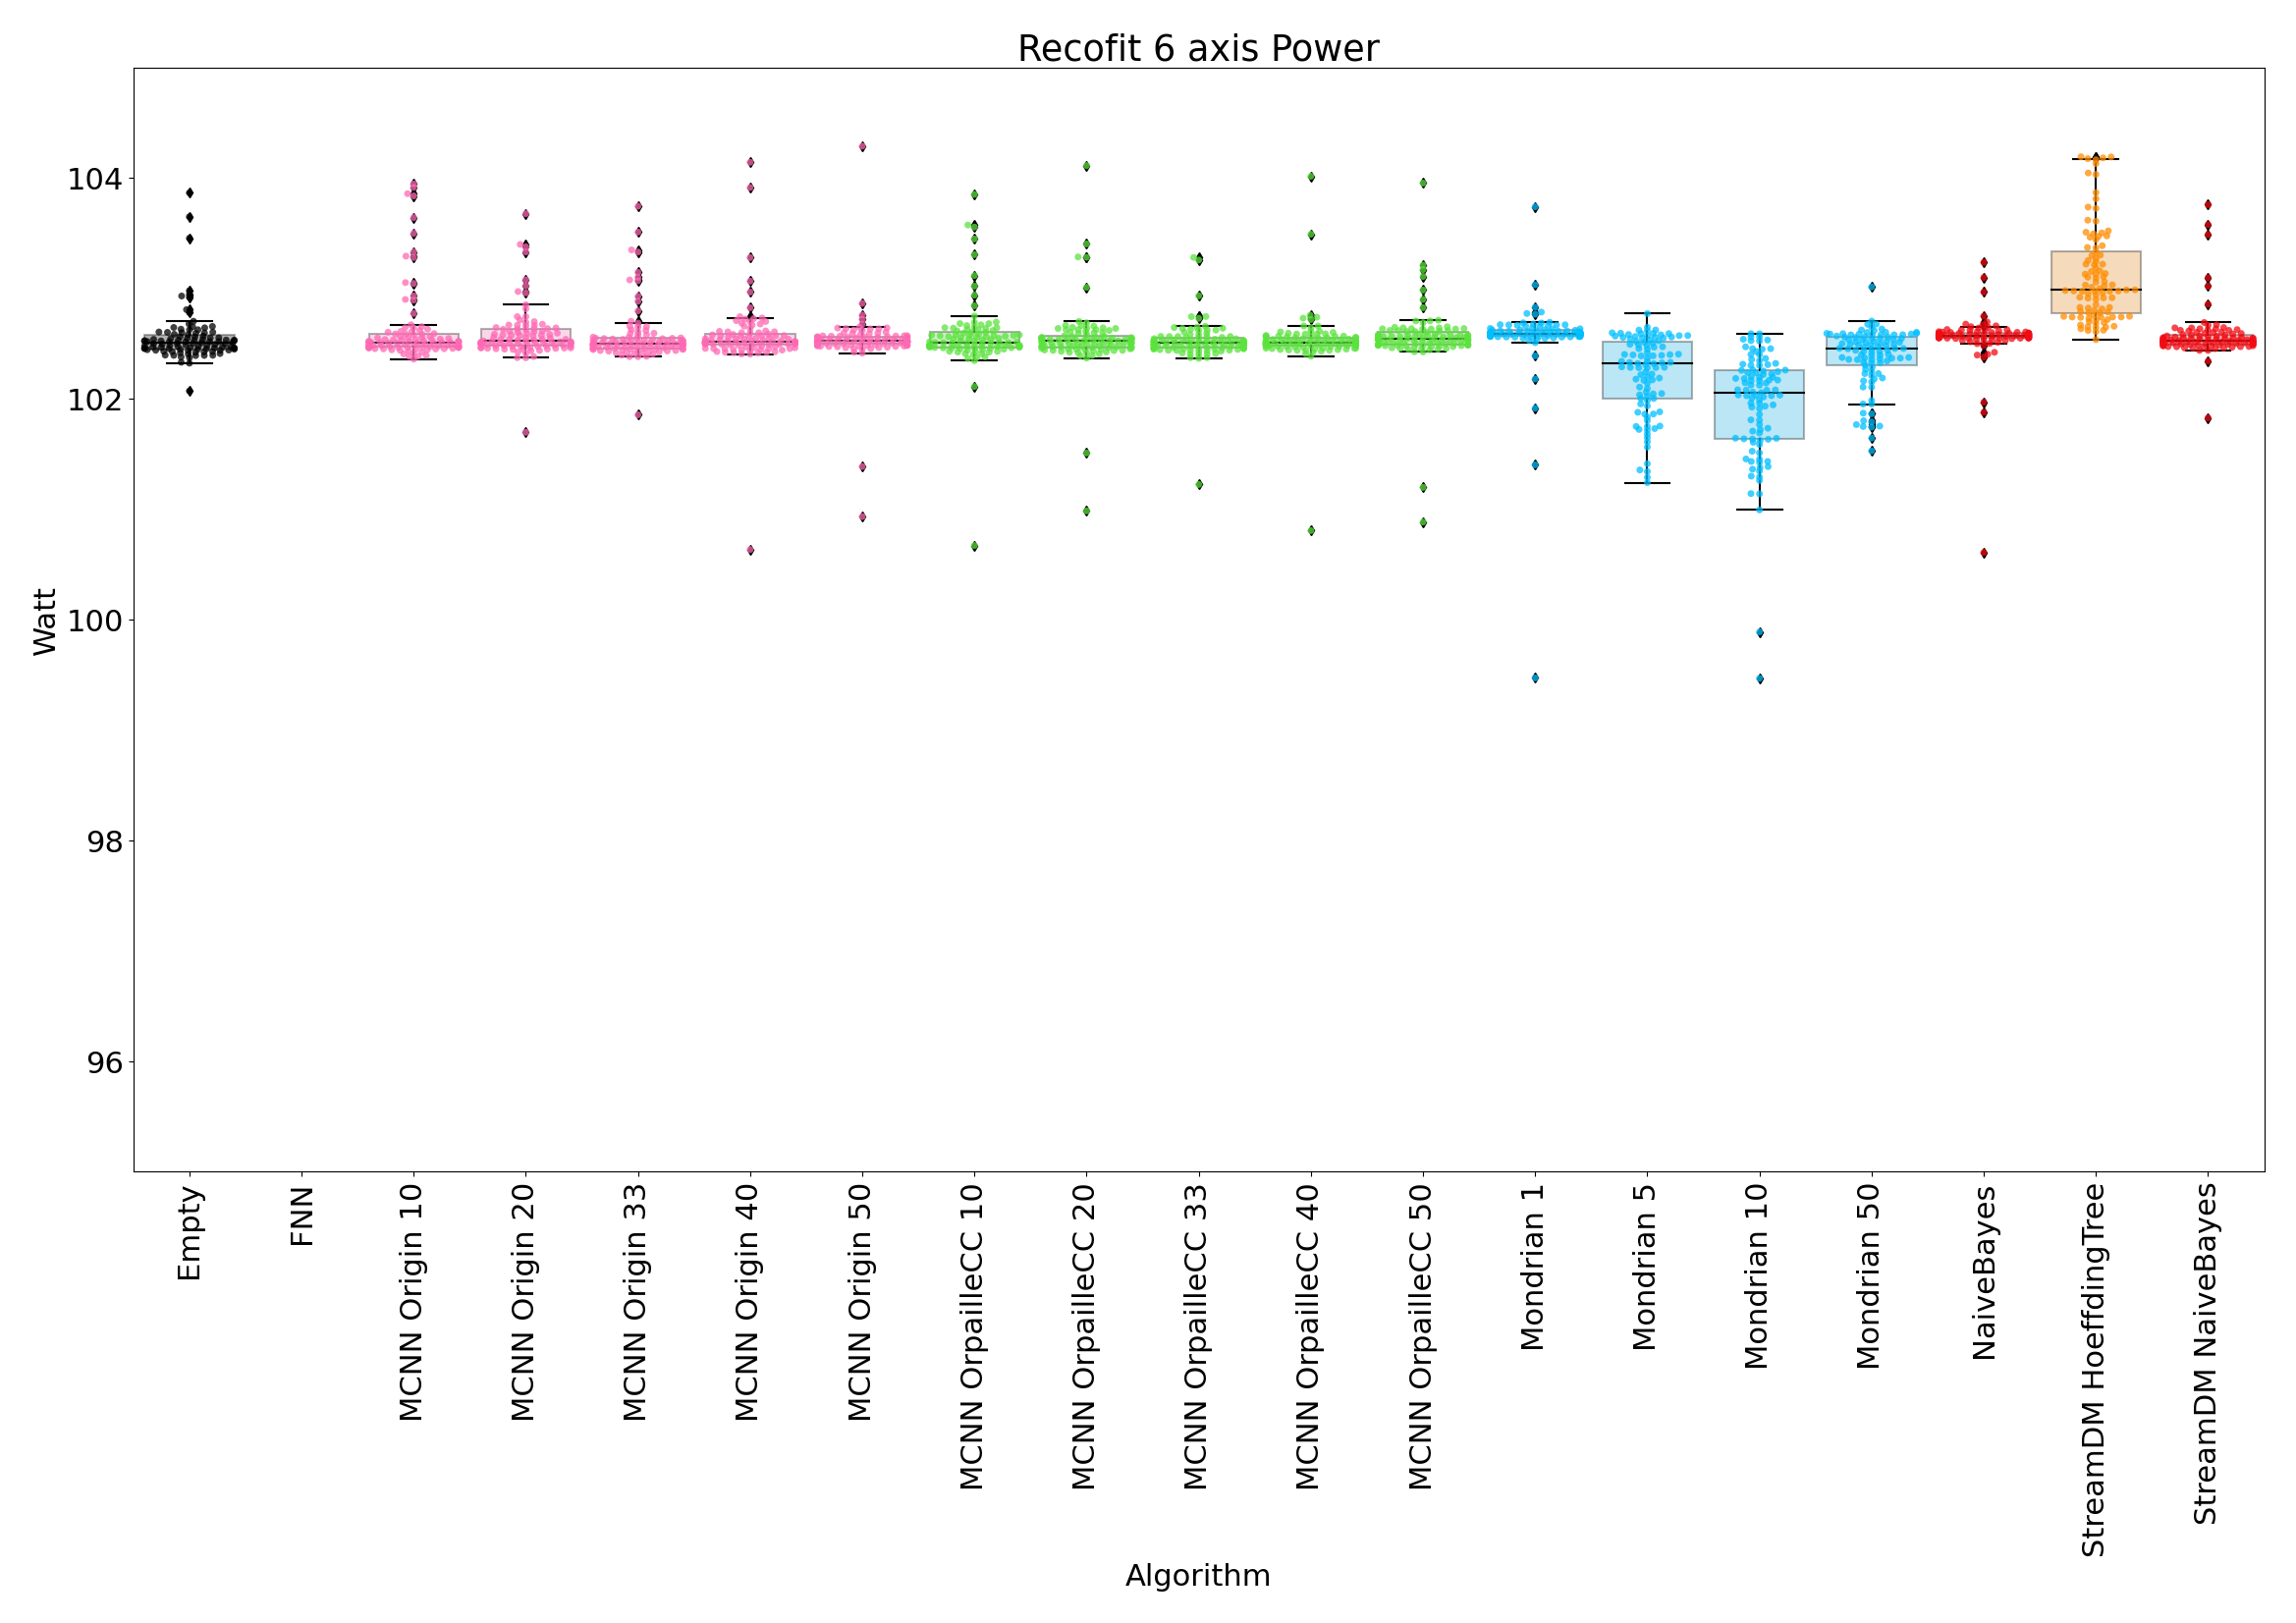
\includegraphics[width=\linewidth]{figures/results/recofit_6_watt.png}
		\caption{\recofitdataset}
		\label{fig:power-recofit}
	\end{subfigure}
	\hfill
	\begin{subfigure}[t]{.49\linewidth}
		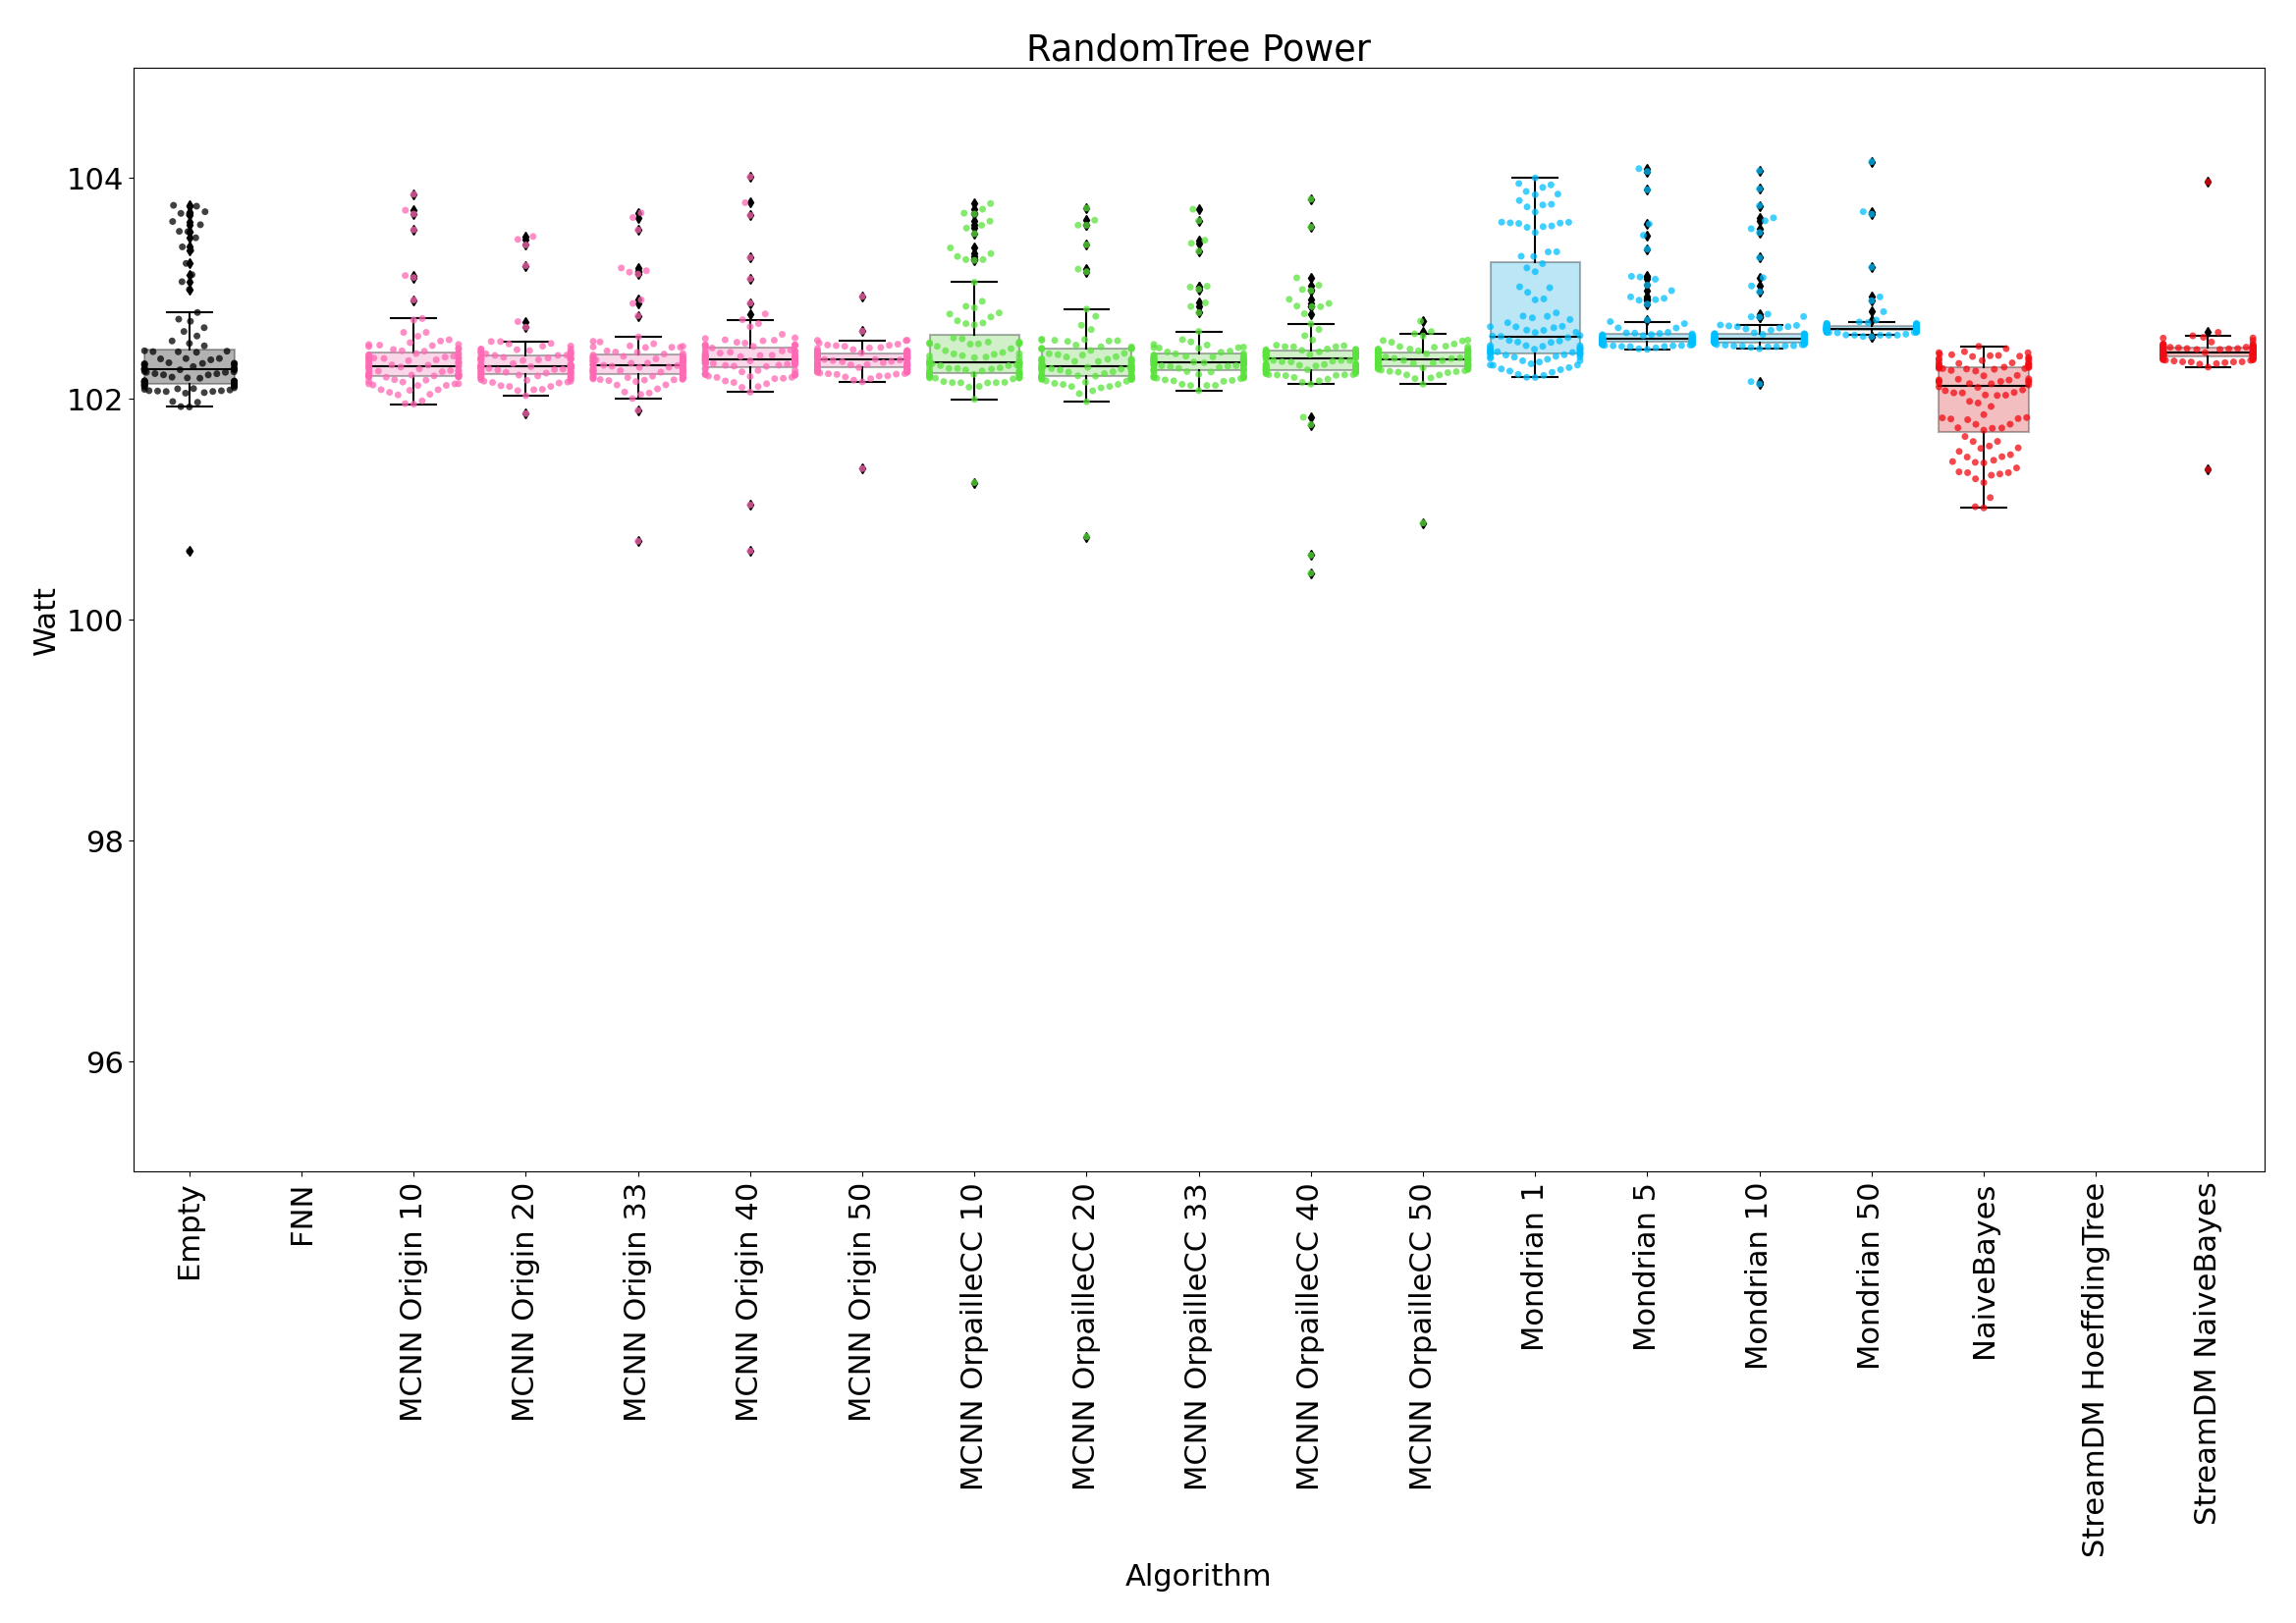
\includegraphics[width=\linewidth]{figures/results/dataset_3_watt.png}
		\caption{RandomTree}
		\label{fig:power-dataset_3}
	\end{subfigure}
	\caption{Power usage for four datasets.}
	\label{fig:power}
\end{figure*}
\subsection{Power}
\label{sec:result-power}
Figure~\ref{fig:power} shows the power usage of each classifier on four
datasets (results are similar for the other two datasets). All classifiers exhibit comparable power consumptions, close to
102~W. Figure~\ref{fig:power-drift} also
shows that the concept drift does not seem to influence power consumption.

This observation is explained by two factors. First, the benchmarking
platform was  working at minimal power. To ensure no disturbance by a
background process, we run the classifiers on an isolated cluster node with
eight cores. Therefore, the power difference on one core is not noticeable.

Another reason are the dataset sizes. Indeed, the slowest run is about
10 seconds with 50 Mondrian trees on \recofitdataset dataset. Such short
executions do not leave time for the CPU to switch P-states because it
barely warms a core. Further experiments would be required to check how 
our power consumption observations generalize to 
connected objects. 

\subsection{Runtime}

Figure~\ref{fig:runtime} shows the classifier runtimes for the two real
datasets. The \mondrianforest is the slowest classifier, in particular for 50
trees. The second slowest classifier is the \hoeffdingtree, with a runtime
comparable to the \mondrianforest with 10 trees. The \hoeffdingtree is followed
by the two \naivebayes implementations, which is not surprising since
\naivebayes classifiers are used in the leaves of the \hoeffdingtree. The \mcnn
classifiers are the fastest ones, with a runtime very close to the empty
classifier. Note that allocating more memory to the \mondrianforest
substantially increases runtime.

We observe that the runtime of StreamDM's \naivebayes is comparable to
OrpailleCC's. This suggests that the performance of the two libraries is
similar, which justifies our comparision of \hoeffdingtree and \mondrianforest.

\begin{figure*}
	\begin{subfigure}[t]{.49\linewidth}
		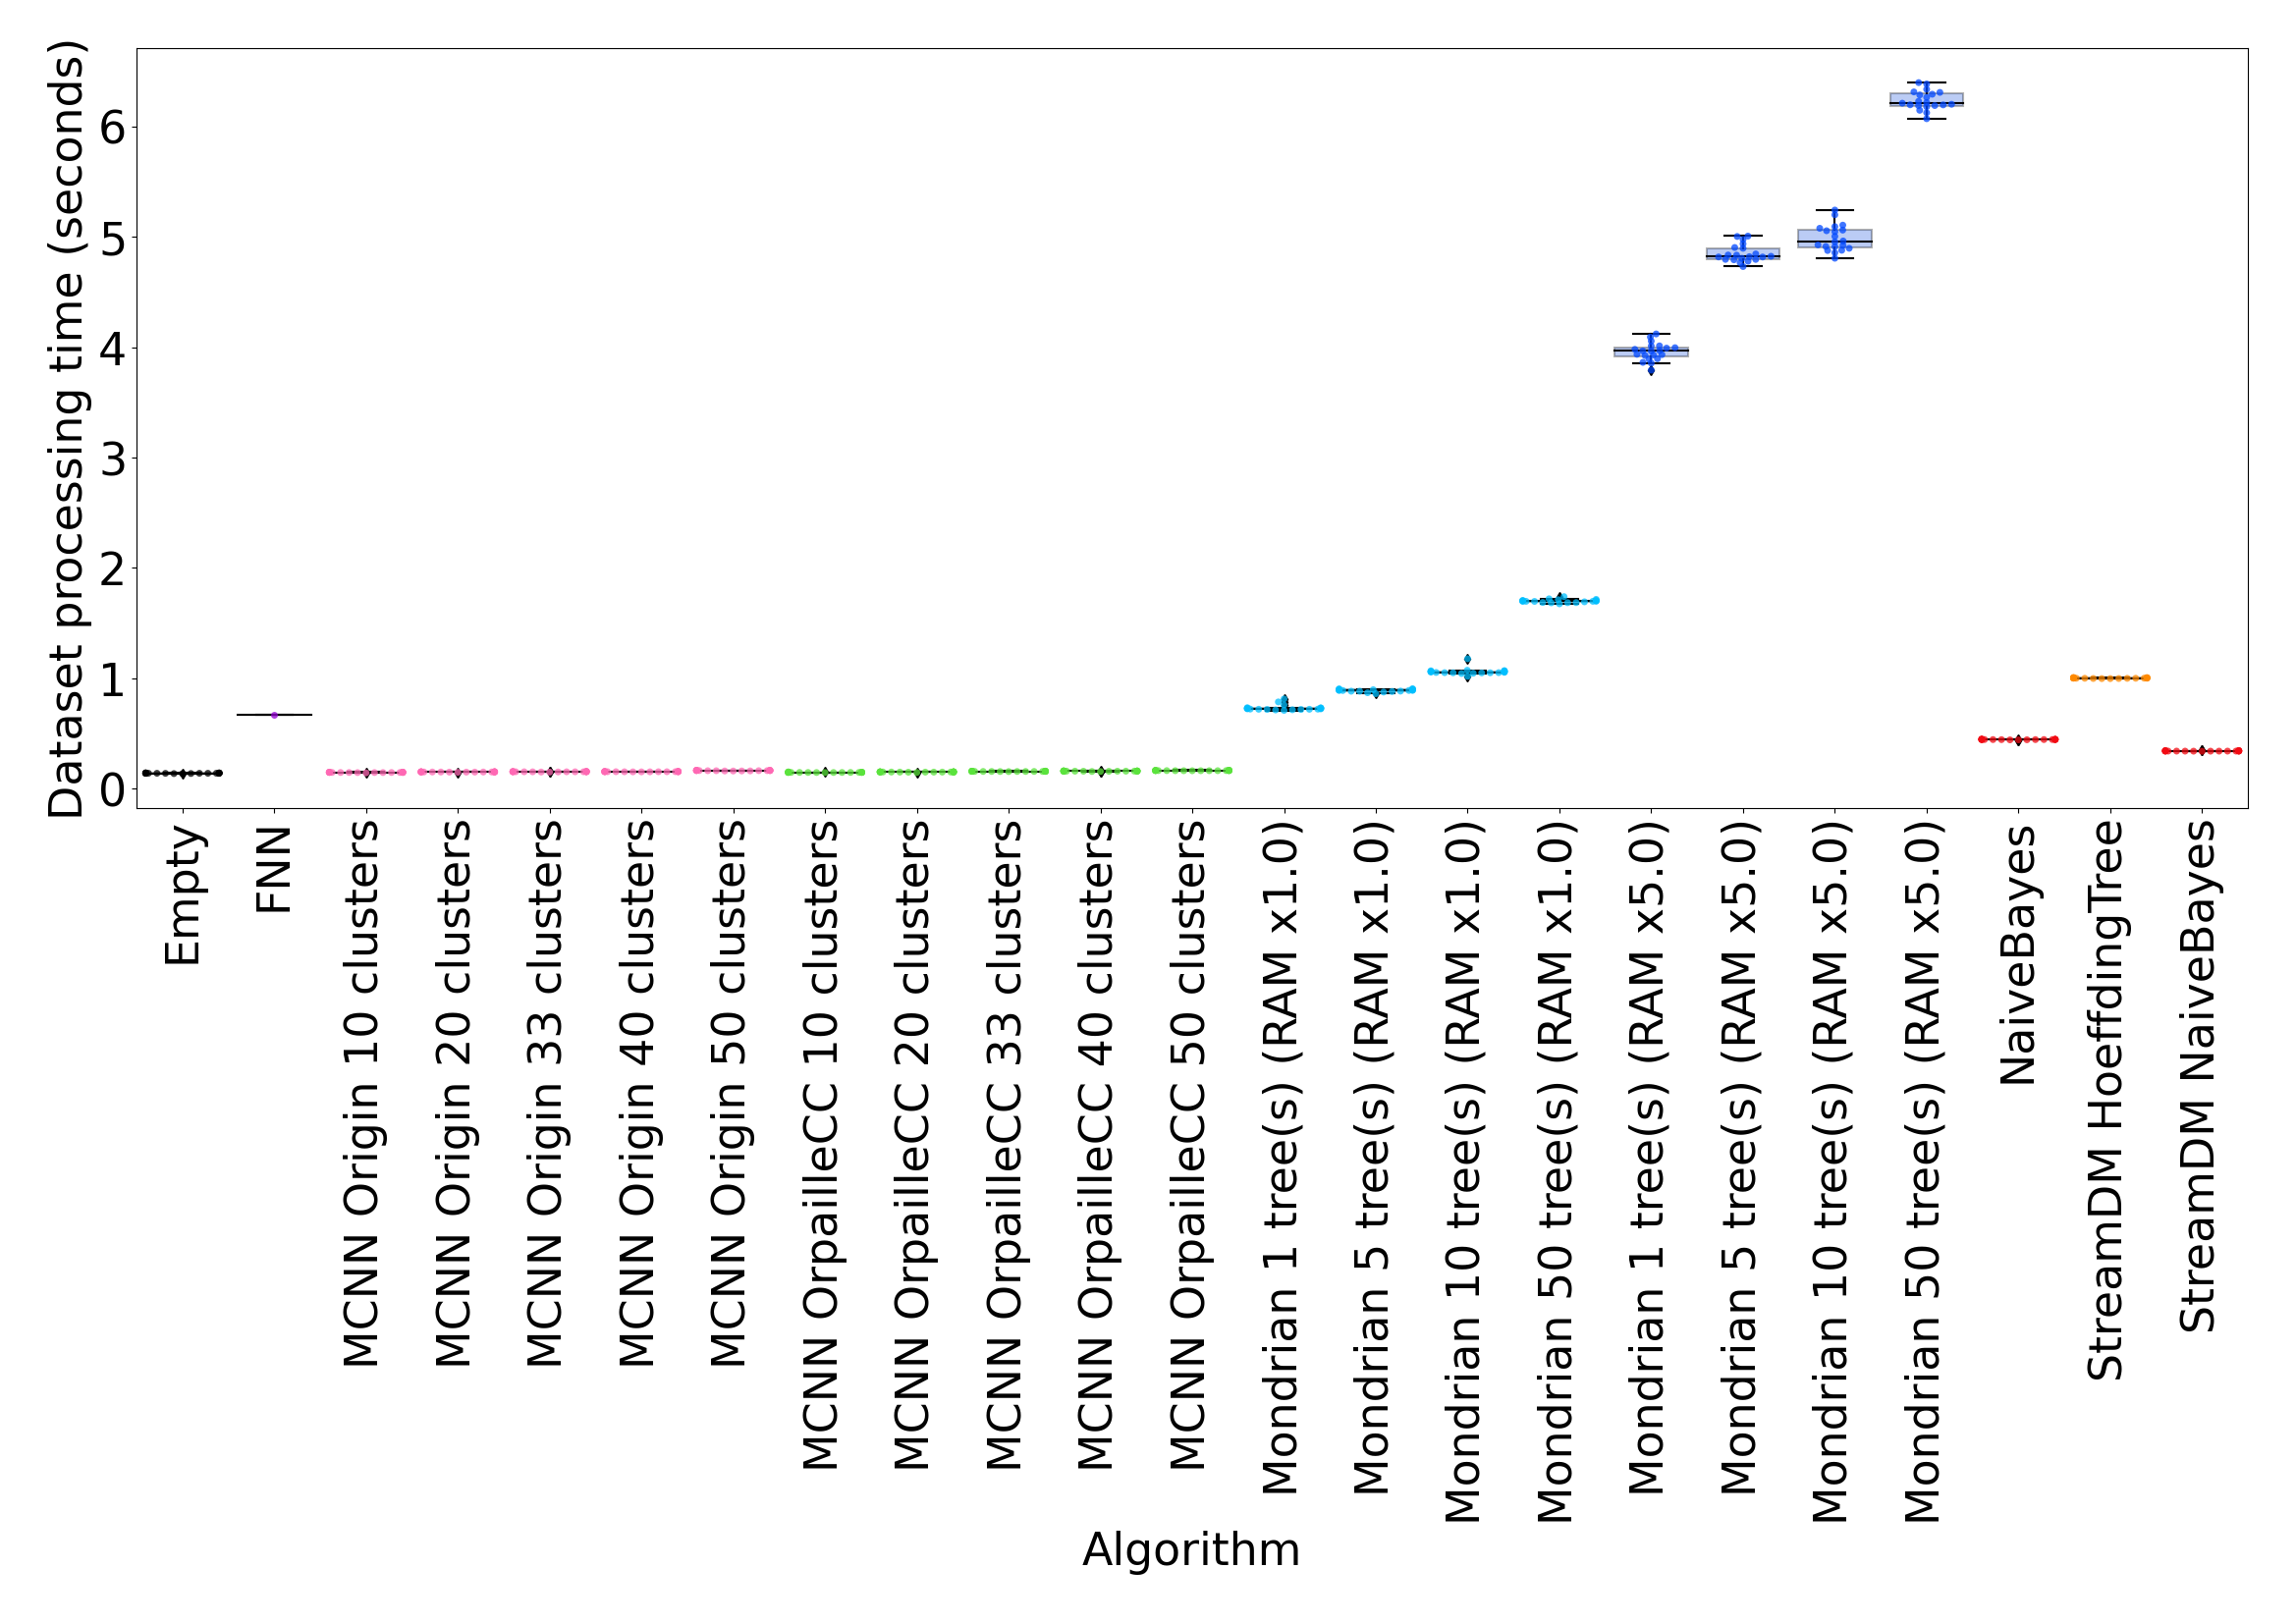
\includegraphics[width=\linewidth]{figures/results/banos_6_runtime.png}
		\caption{\banosdataset}
		\label{fig:runtime-banos}
	\end{subfigure}
	\hfill
	\begin{subfigure}[t]{.49\linewidth}
		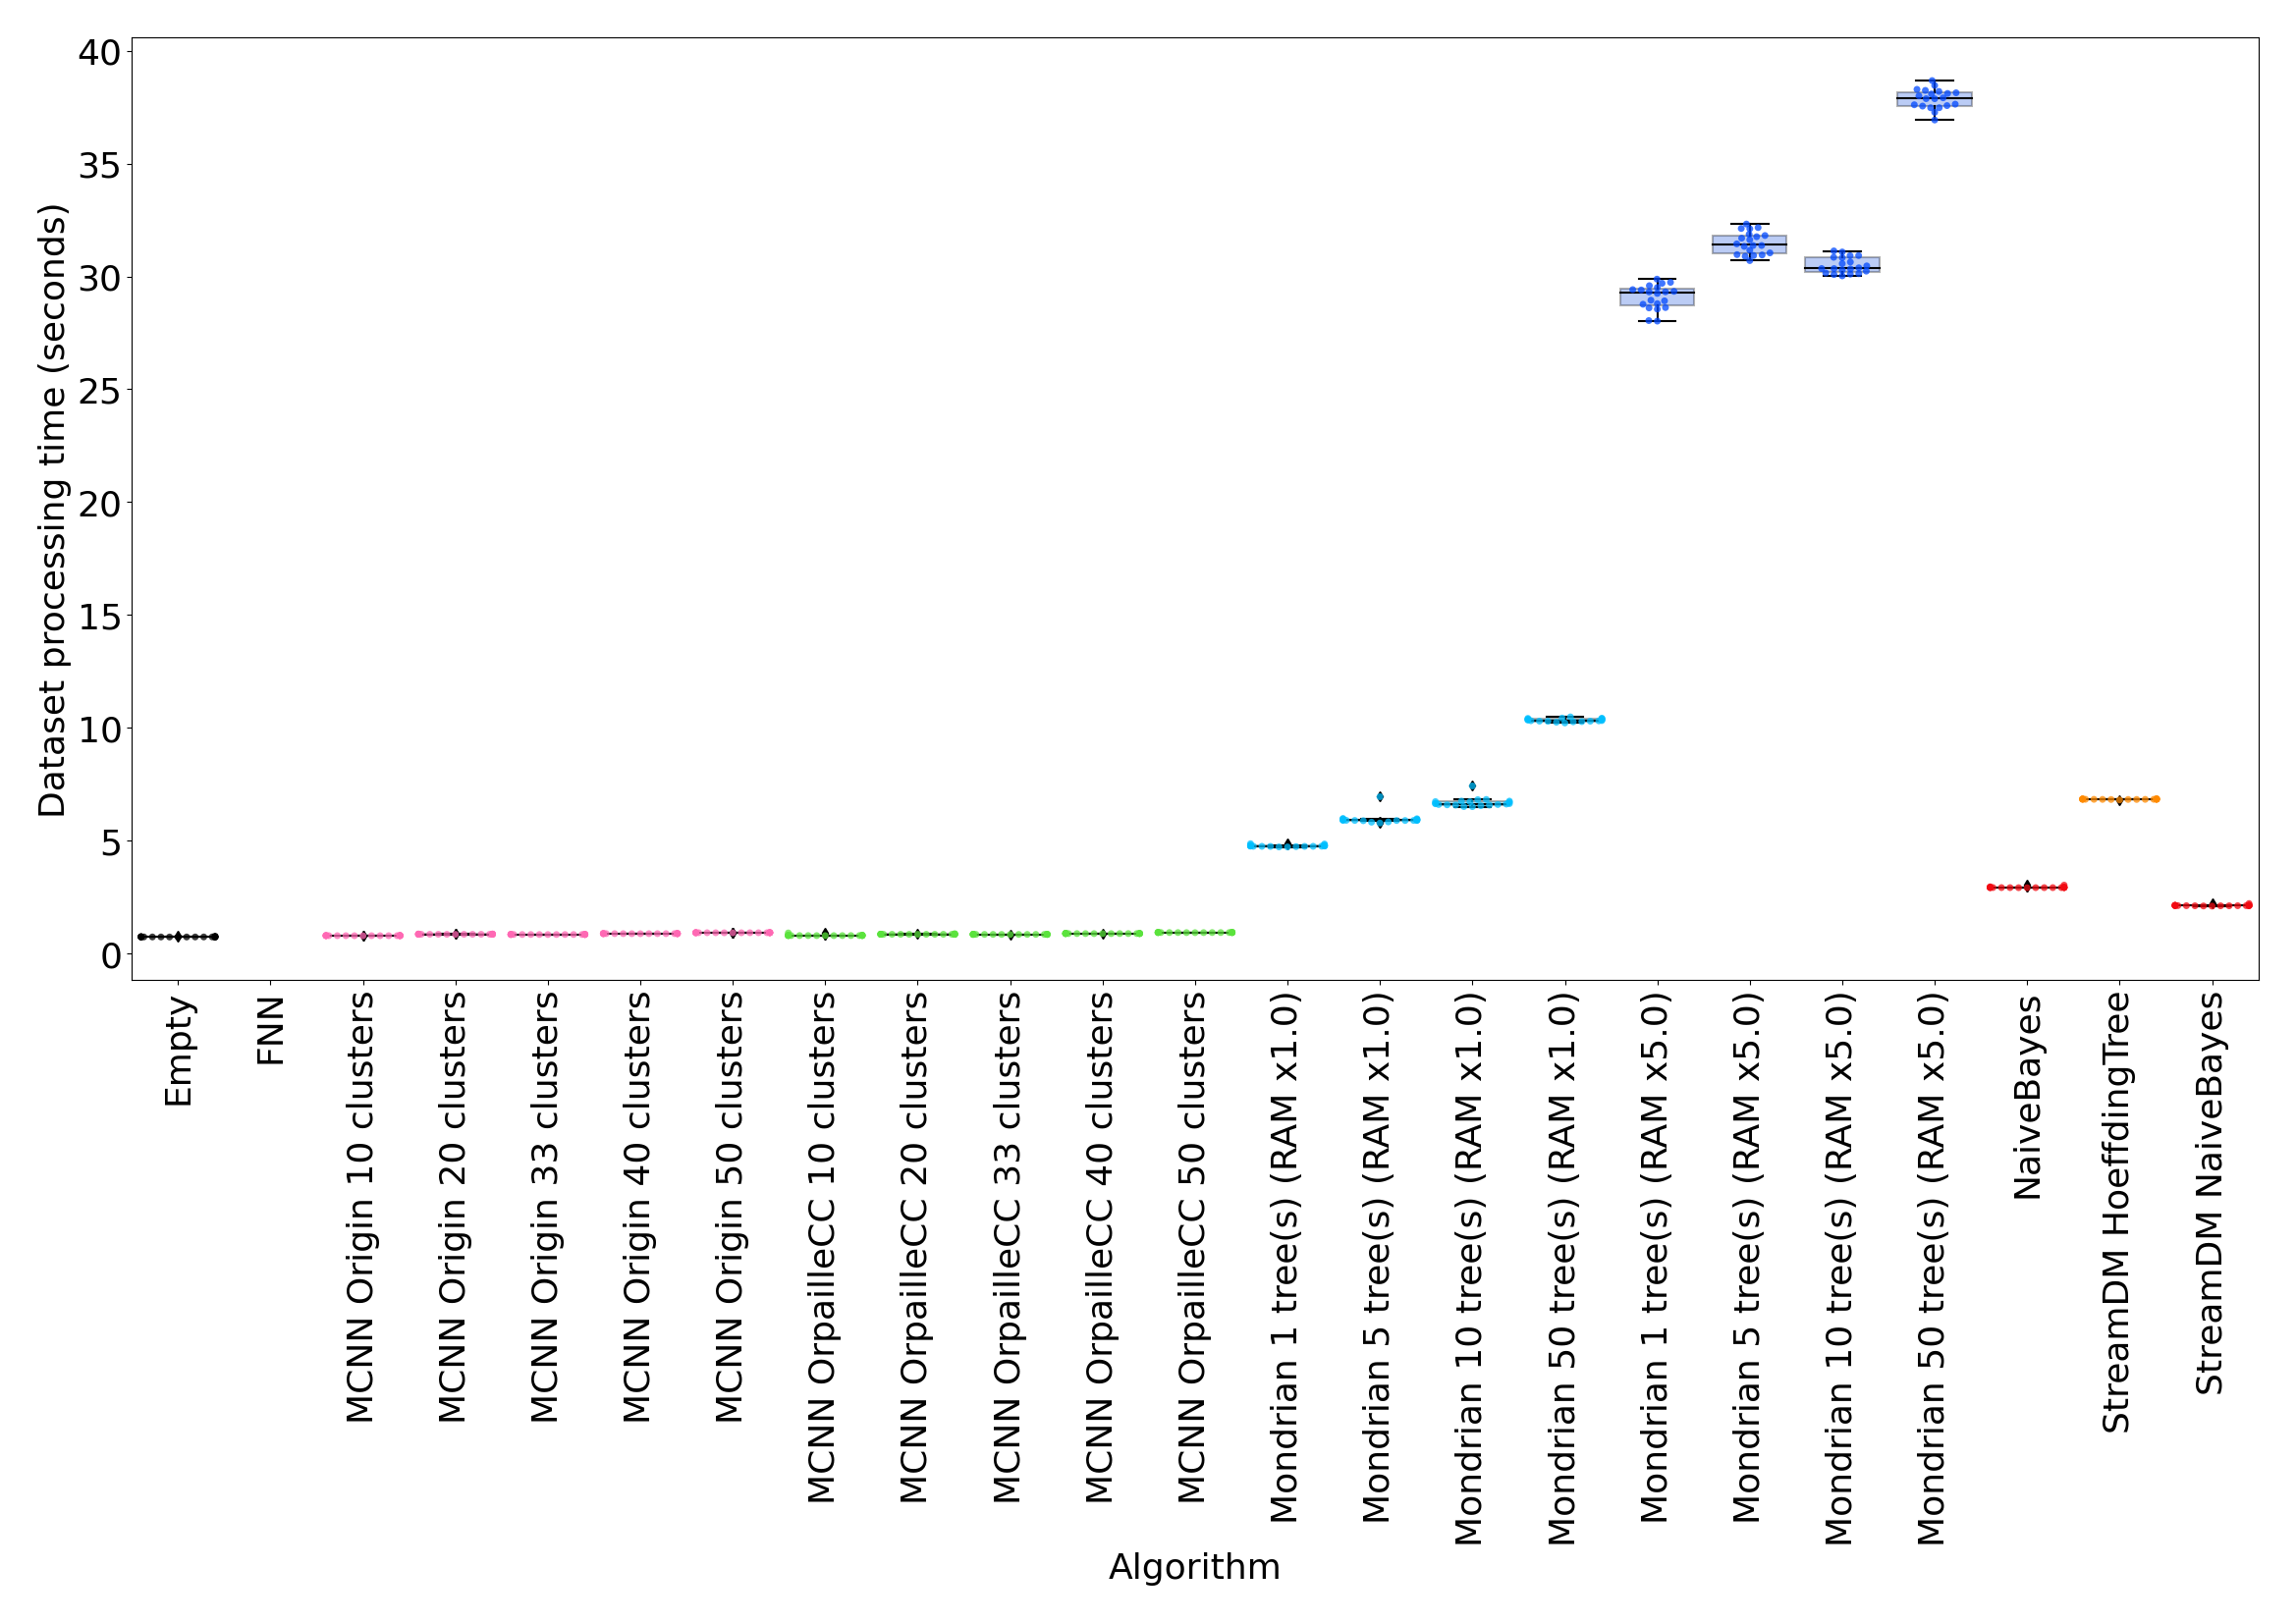
\includegraphics[width=\linewidth]{figures/results/recofit_6_runtime.png}
		\caption{\recofitdataset}
		\label{fig:runtime-recofit}
	\end{subfigure}
	\caption{Runtime with the two real datasets (20 repetitions).}
	\label{fig:runtime}
\end{figure*}

\subsection{Memory}
\label{sec:result-memory}
Figure~\ref{fig:memory} shows the evolution of the memory footprint for the
\banosdataset dataset. Results are similar for the other datasets and are
not reported for brevity. Since the  memory footprint of the \naivebayes
classifier was almost indistinguishable from the empty classifier, we used
the two \naivebayes as a baseline for the two libraries. This enables us to
remove the 1.2~MB overhead induced by StreamDM. The StreamDM memory
footprint matches the result in~\cite{StreamDM-CPP}, where the
\hoeffdingtree shows a memory footprint of 4.8MB.

We observe that the memory footprints of the \mondrianforest and the
\hoeffdingtree are substantially higher than for the other classifiers, which makes 
their deployment on connected objects challenging.
Overall, memory footprints are similar across datasets, due to the
fact that most algorithms follow a bounded memory policy or have a constant
space complexity.  The only exception is the \hoeffdingtree that constantly
selects new splits depending on new data points. The \mondrianforest has the
same behavior but the OrpailleCC implementation is memory-bounded, which
makes its memory footprint constant.
%  The concept drift does not
% increase the memory footprint of the \hoeffdingtree.

\begin{figure}
	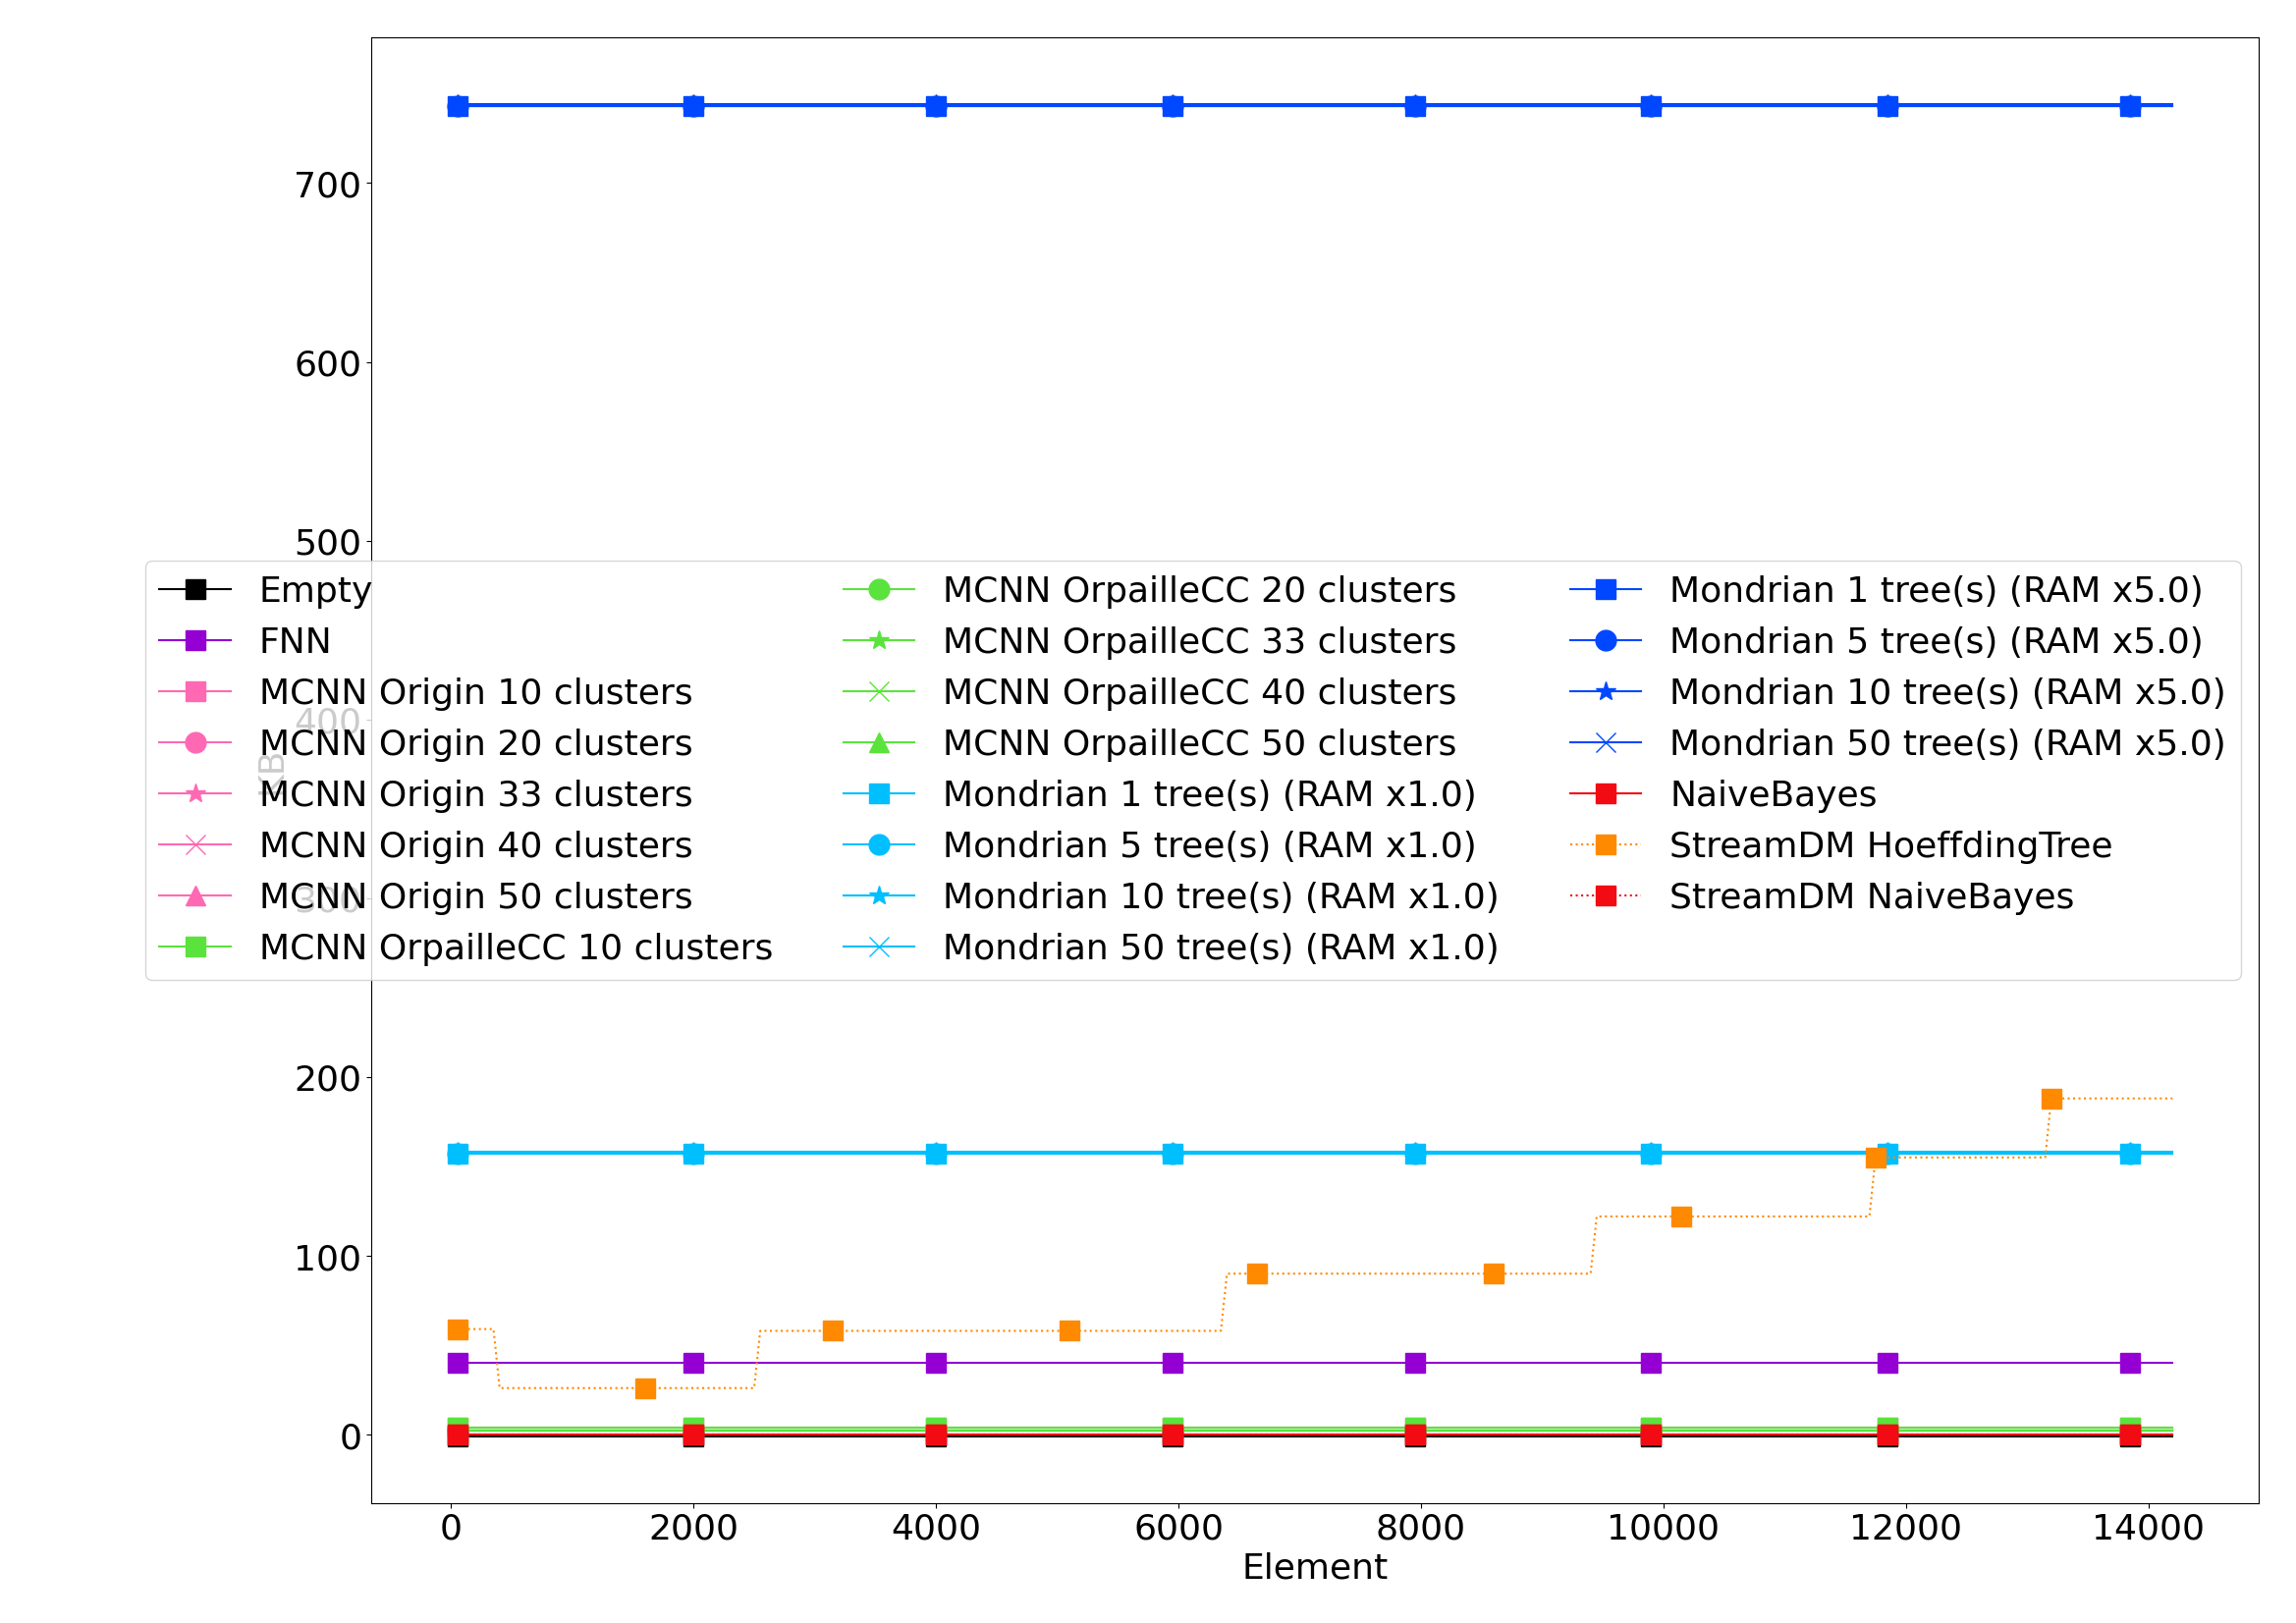
\includegraphics[width=\linewidth]{figures/results/banos_6_memory.png}
	\caption{Memory footprint of the classifiers relatively to the empty
	classifier, measured on the \banosdataset dataset. The memory footprint of the empty
	classifier is 3.439MB. The baselines are the two \naivebayes from OrpailleCC
		and StreamDM. They respectively have a memory footprint of 3.44OMB and
		4.743.}
	\label{fig:memory}
\end{figure}


\subsection{Hyperparameter tuning}

Figure~\ref{fig:mcnn-tuning-error} shows the impact of the error threshold
in the \mcnn classifiers with different cluster counts. The error
threshold of \mcnn has little impact on the classification performance. For
20 and 40 clusters, the best-performing threshold is either 2 or 4, meaning
that a cluster may do 2 or 4 errors before being split. For 10 clusters,
all error thresholds perform equally.

\begin{figure}
	 \begin{subfigure}[b]{0.49\textwidth}
		 \centering
		 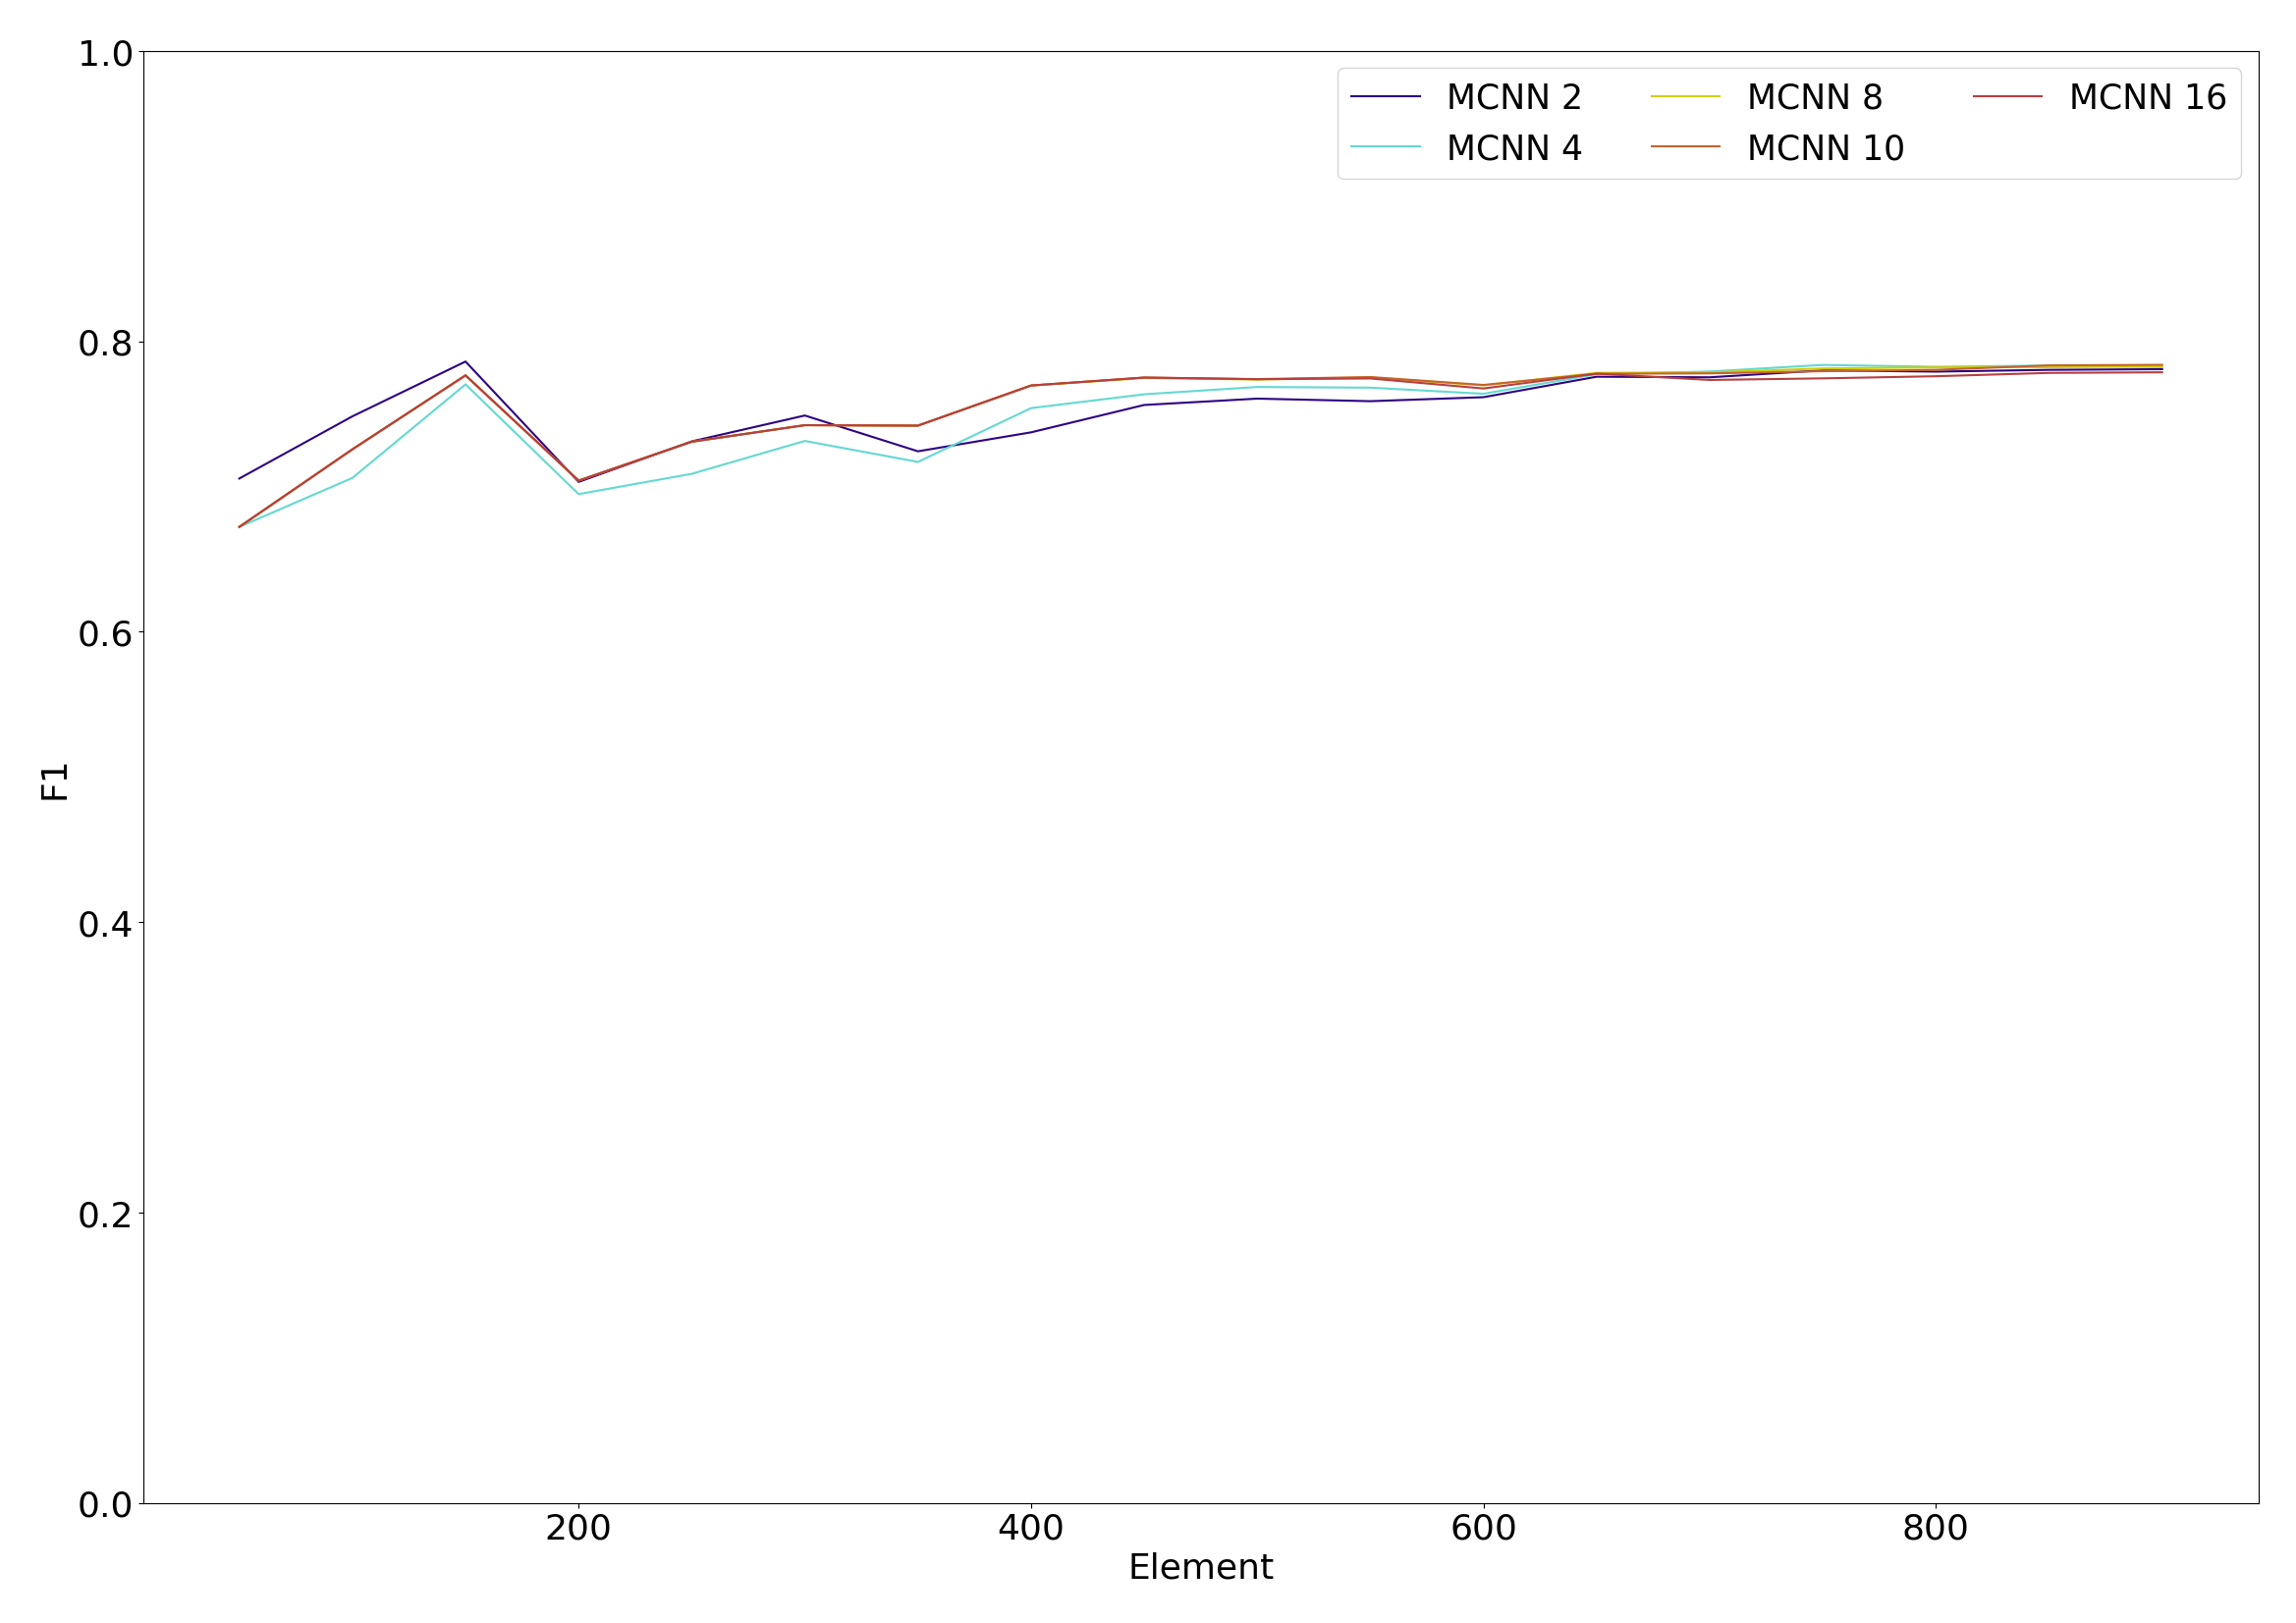
\includegraphics[width=\linewidth]{figures/calibration_mcnn_40.png}
		 \caption{40 clusters}
	 \end{subfigure}
	 \begin{subfigure}[b]{0.49\textwidth}
		 \centering
		 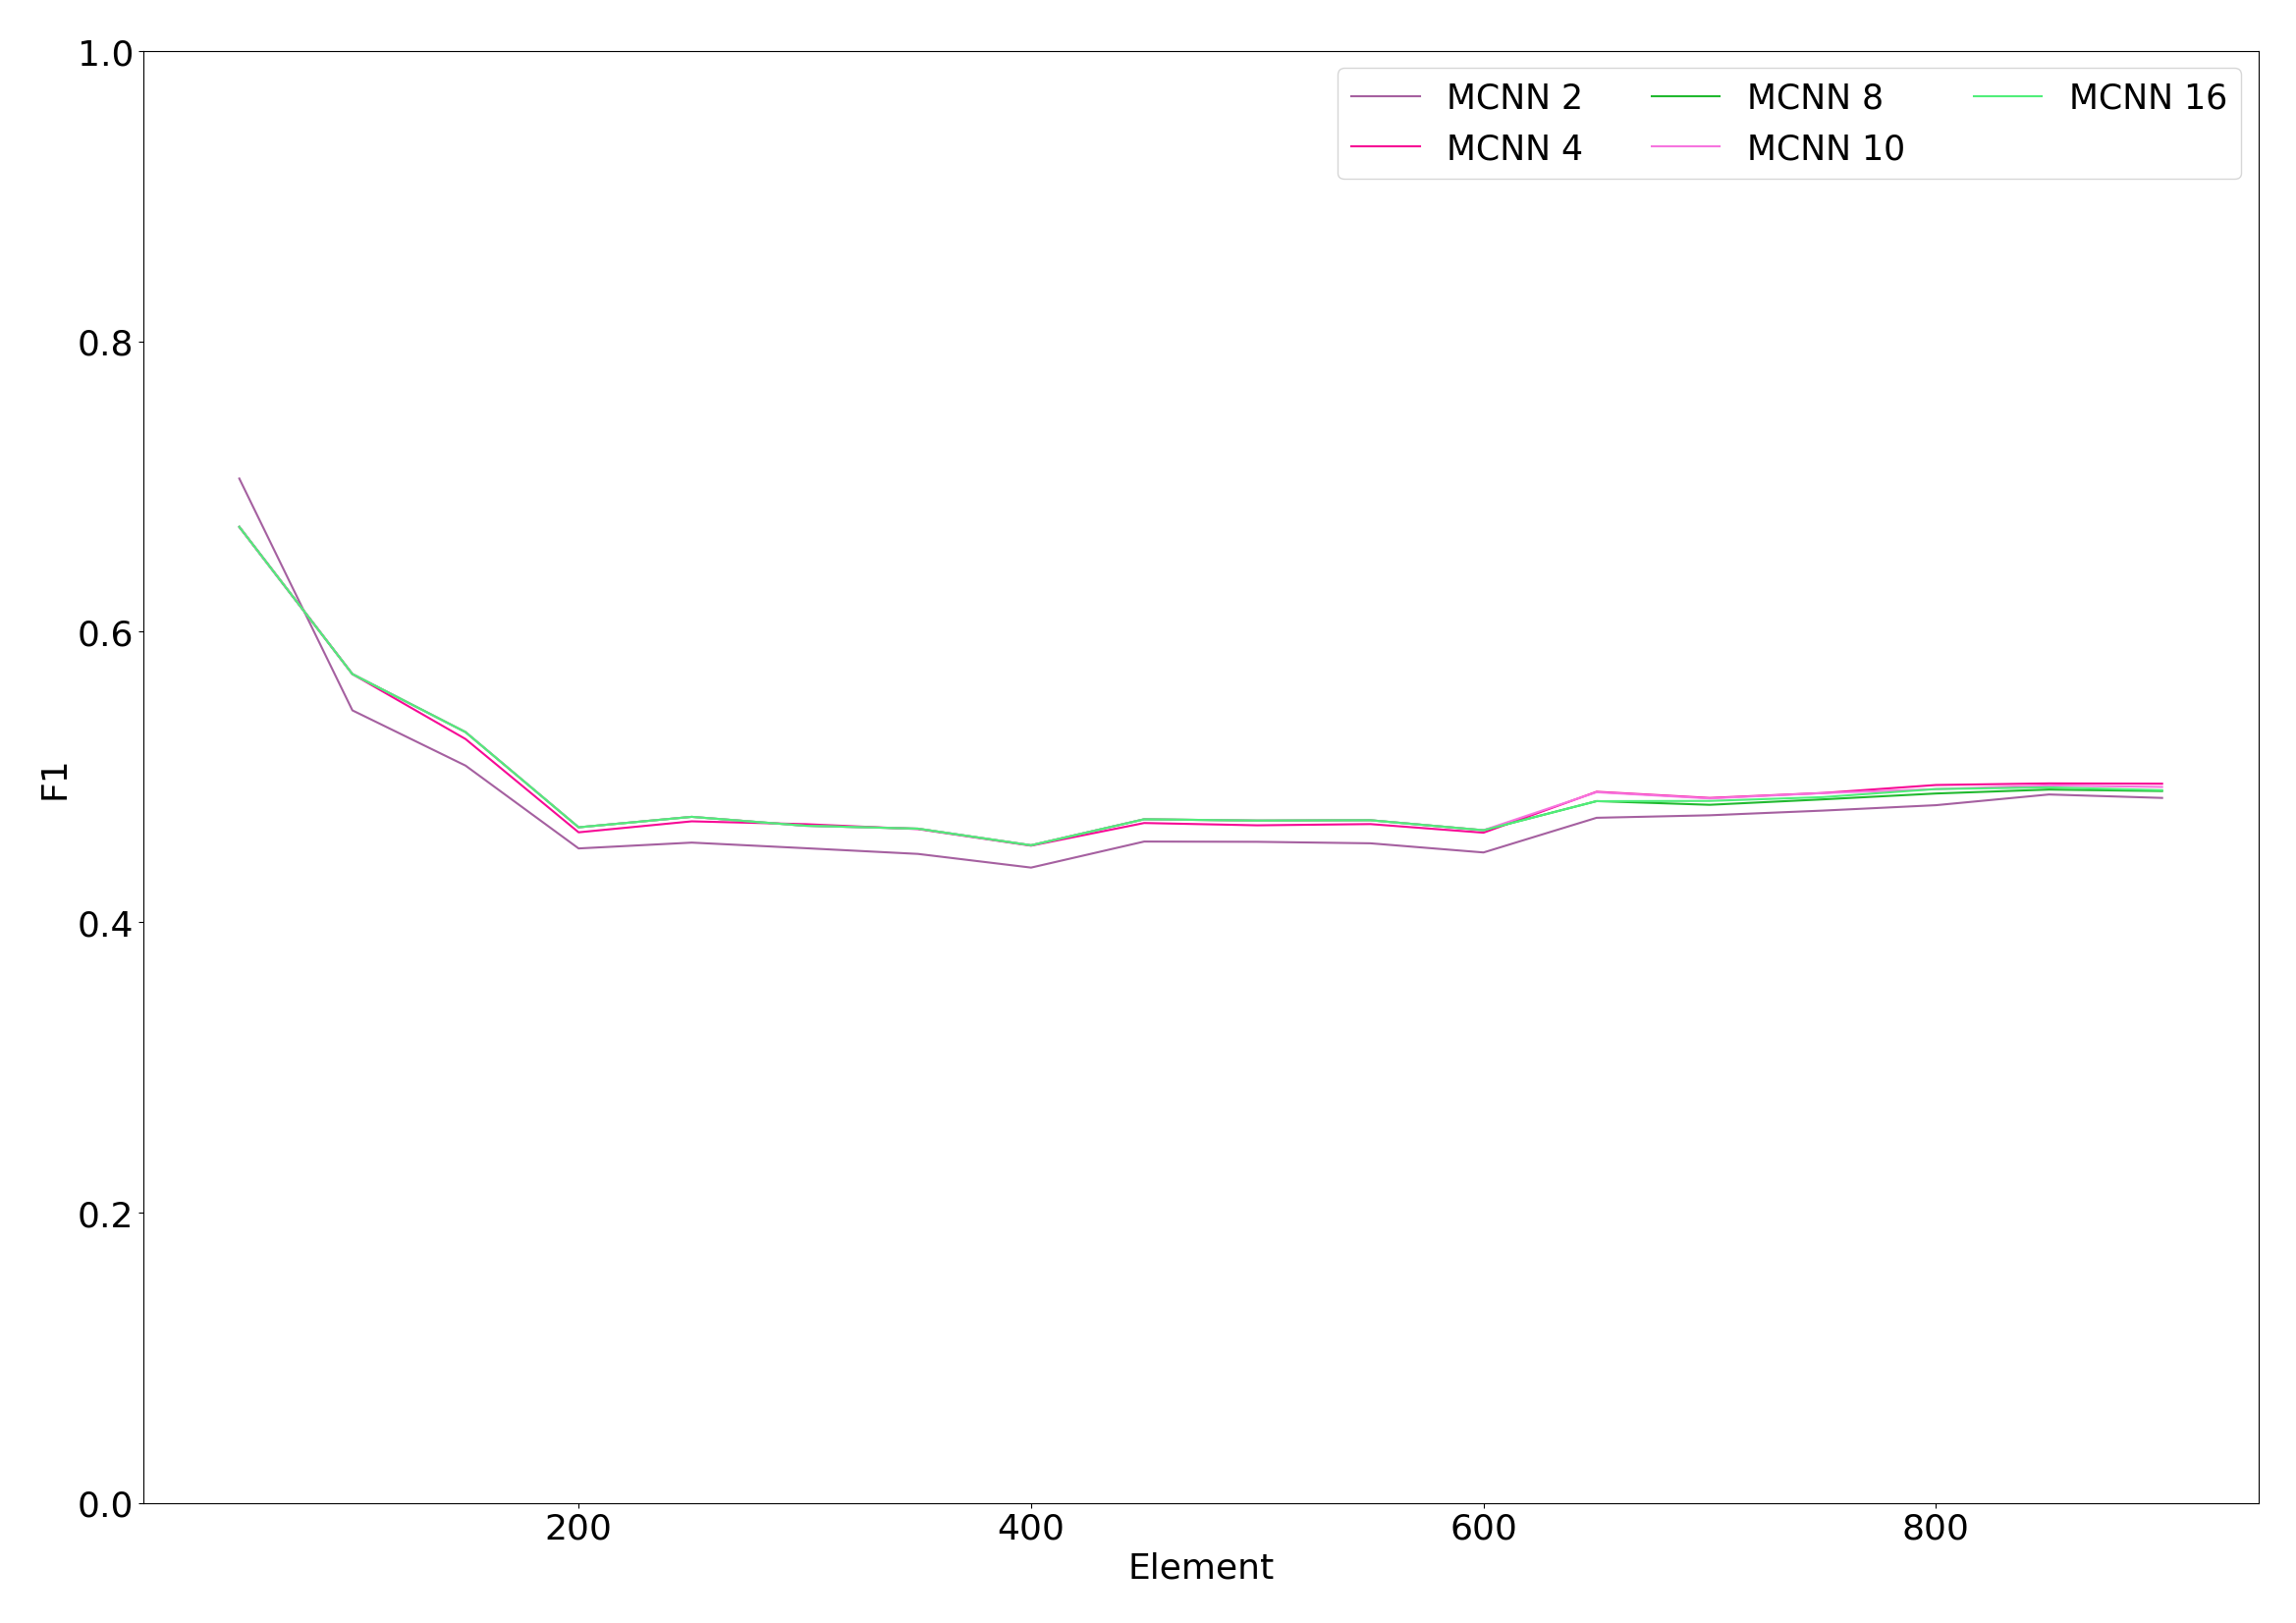
\includegraphics[width=\linewidth]{figures/calibration_mcnn_20.png}
		 \caption{20 clusters}
	 \end{subfigure}
	 \begin{subfigure}[b]{0.49\textwidth}
		 \centering
		 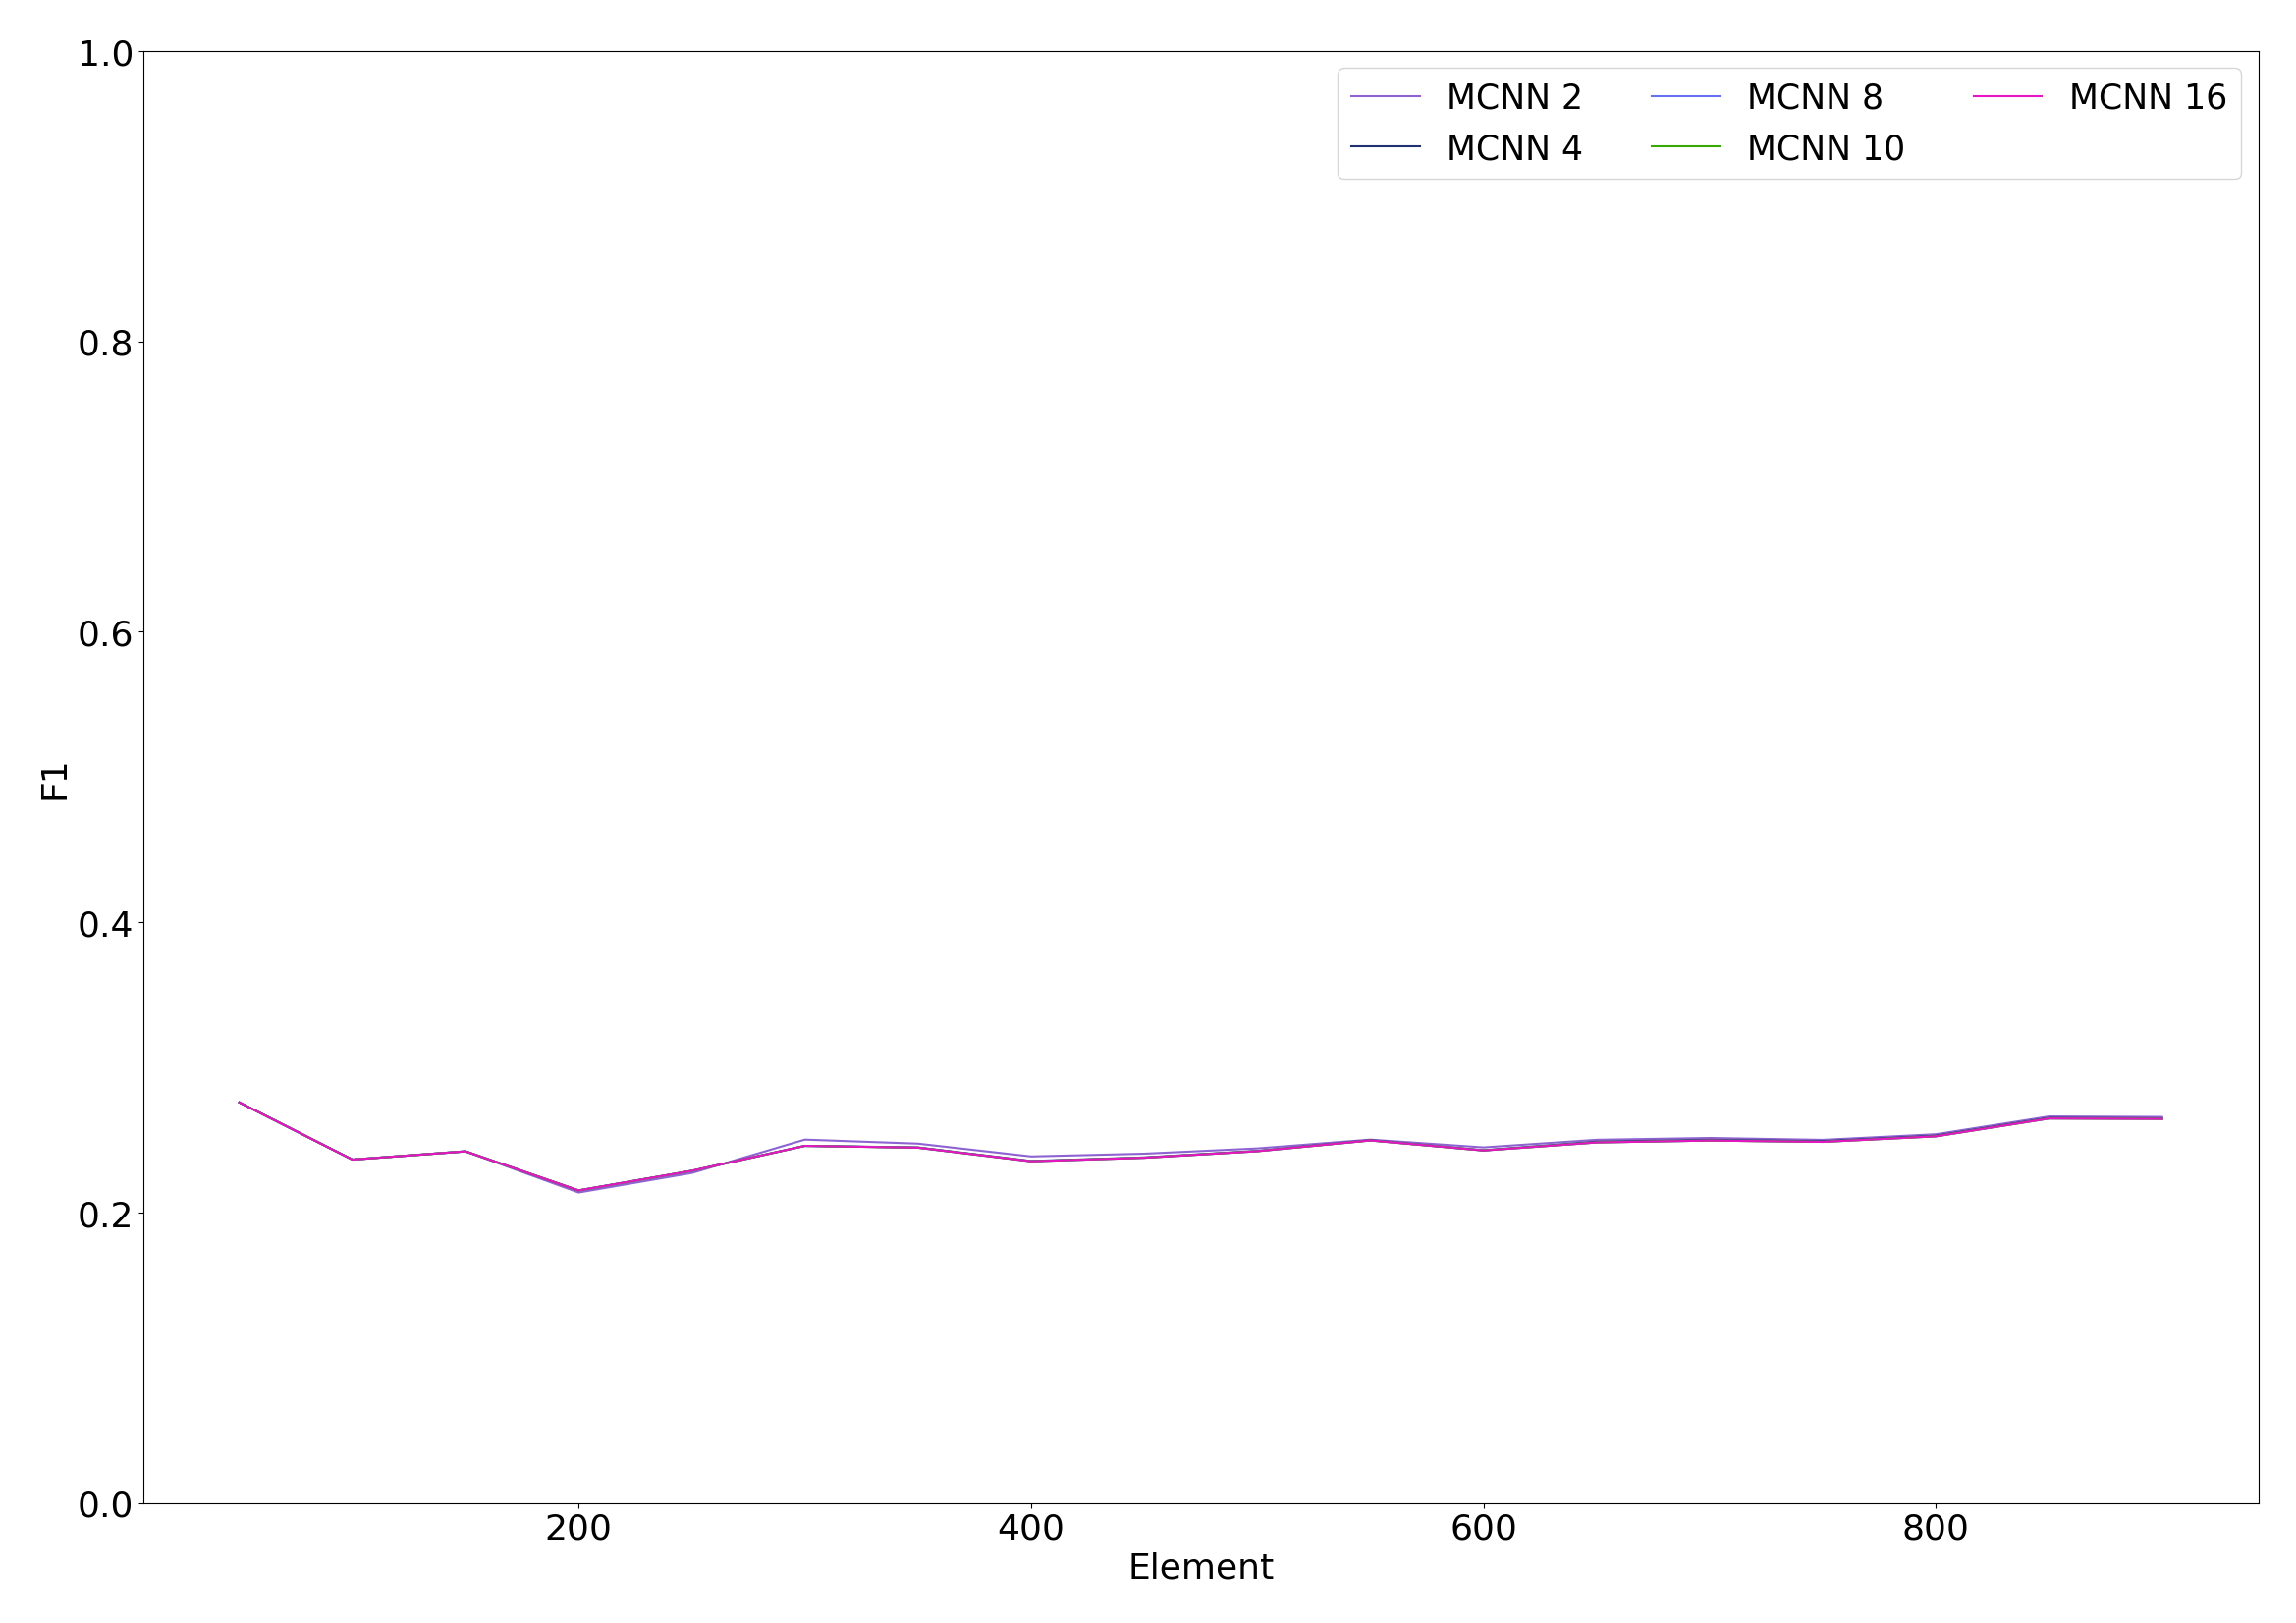
\includegraphics[width=\linewidth]{figures/calibration_mcnn_10.png}
		 \caption{10 clusters}
	 \end{subfigure}
	\caption{Error threshold tuning of \mcnn with first subject of \banosdataset dataset.}
	\label{fig:mcnn-tuning-error}
\end{figure}

Figure~\ref{fig:mondrian-tuning} shows the impact of the \mondrianforest hyperparameters on
the classification performance. 
The base count hyperparameter (Figure~\ref{fig:mondrian-base-count}) has a
very substantial impact on classification performance; the smallest value
(0.0) results in the best performance. On the contrary, the
budget hyperparameter (Figure~\ref{fig:mondrian-budget}) only has a
moderate impact on classification; the best value is 0.2. Finally, the discount hyperparameter
(Figure~\ref{fig:mondrian-discount}) has a negligible impact on the
performance; the best-performing value is 0.1.

\begin{figure}
	 \centering
	 \begin{subfigure}[b]{0.49\textwidth}
		\centering
		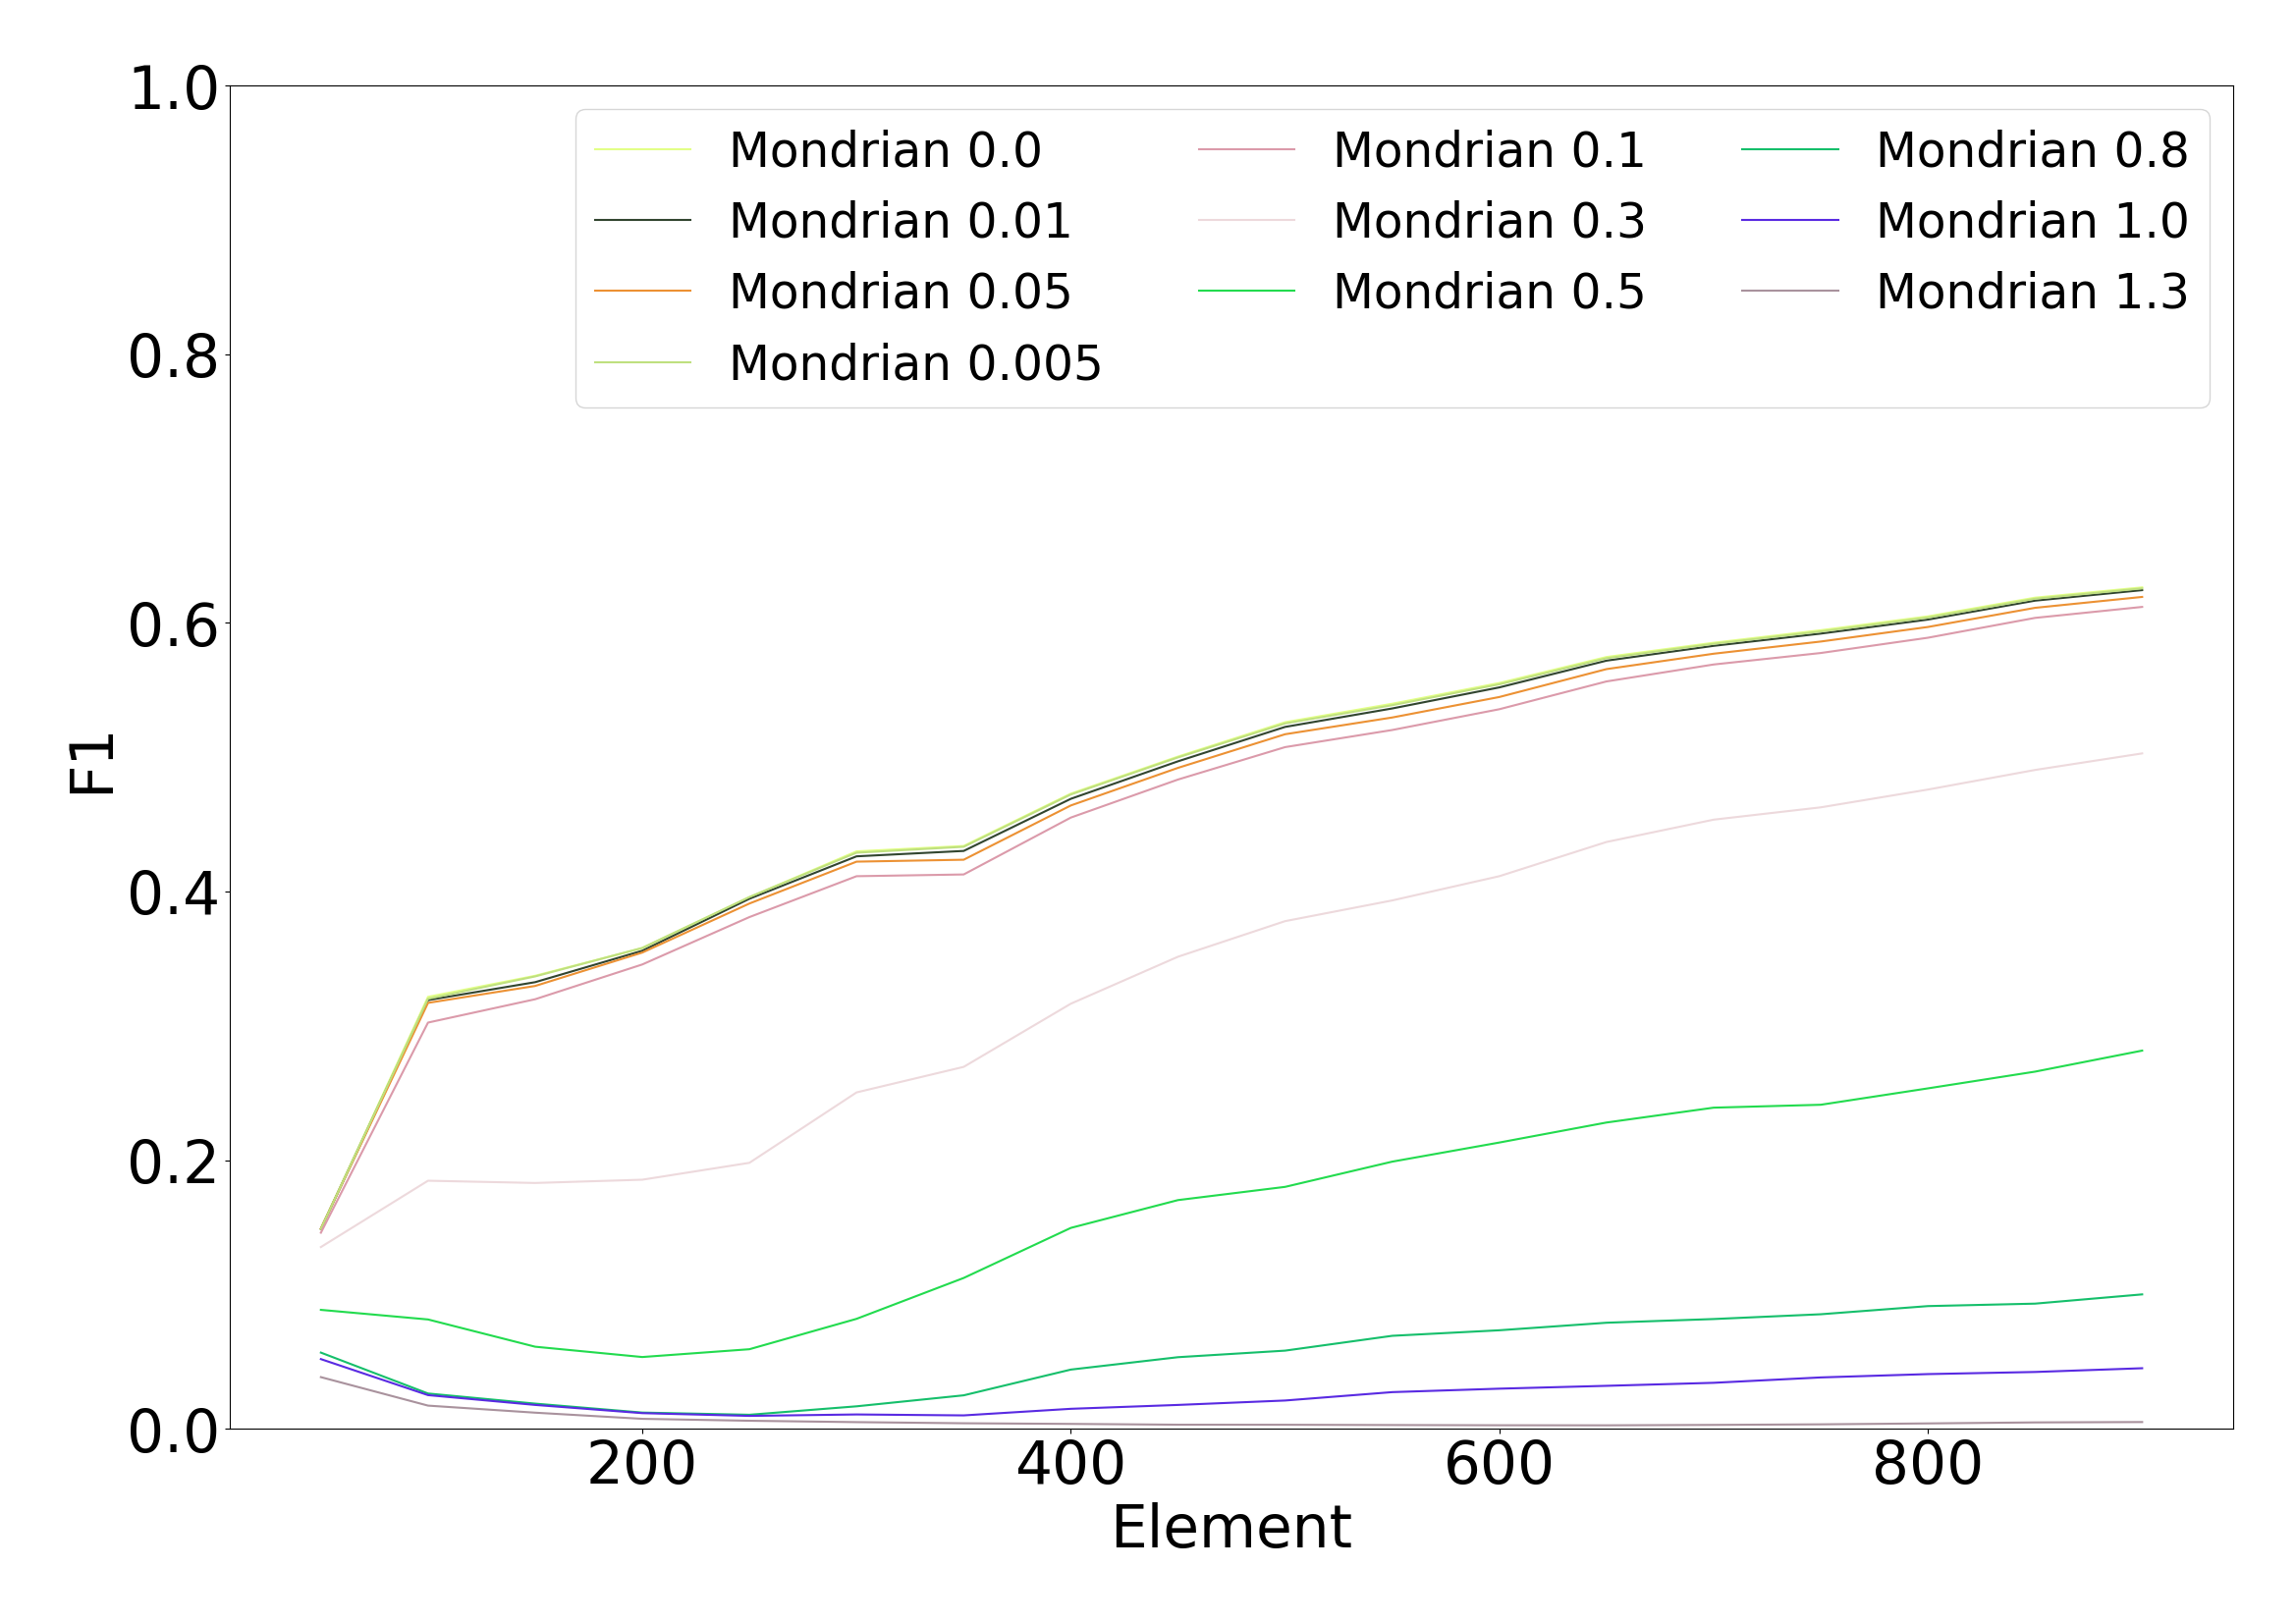
\includegraphics[width=\textwidth]{figures/calibration_mondrian_base.png}
		\caption{Impact of the base count with 10 trees, a budget of $1.0$, and a discount factor of $0.2$.} 
		\label{fig:mondrian-base-count}
	\end{subfigure}
	\hfill
	 \begin{subfigure}[b]{0.49\textwidth}
		 \centering
		 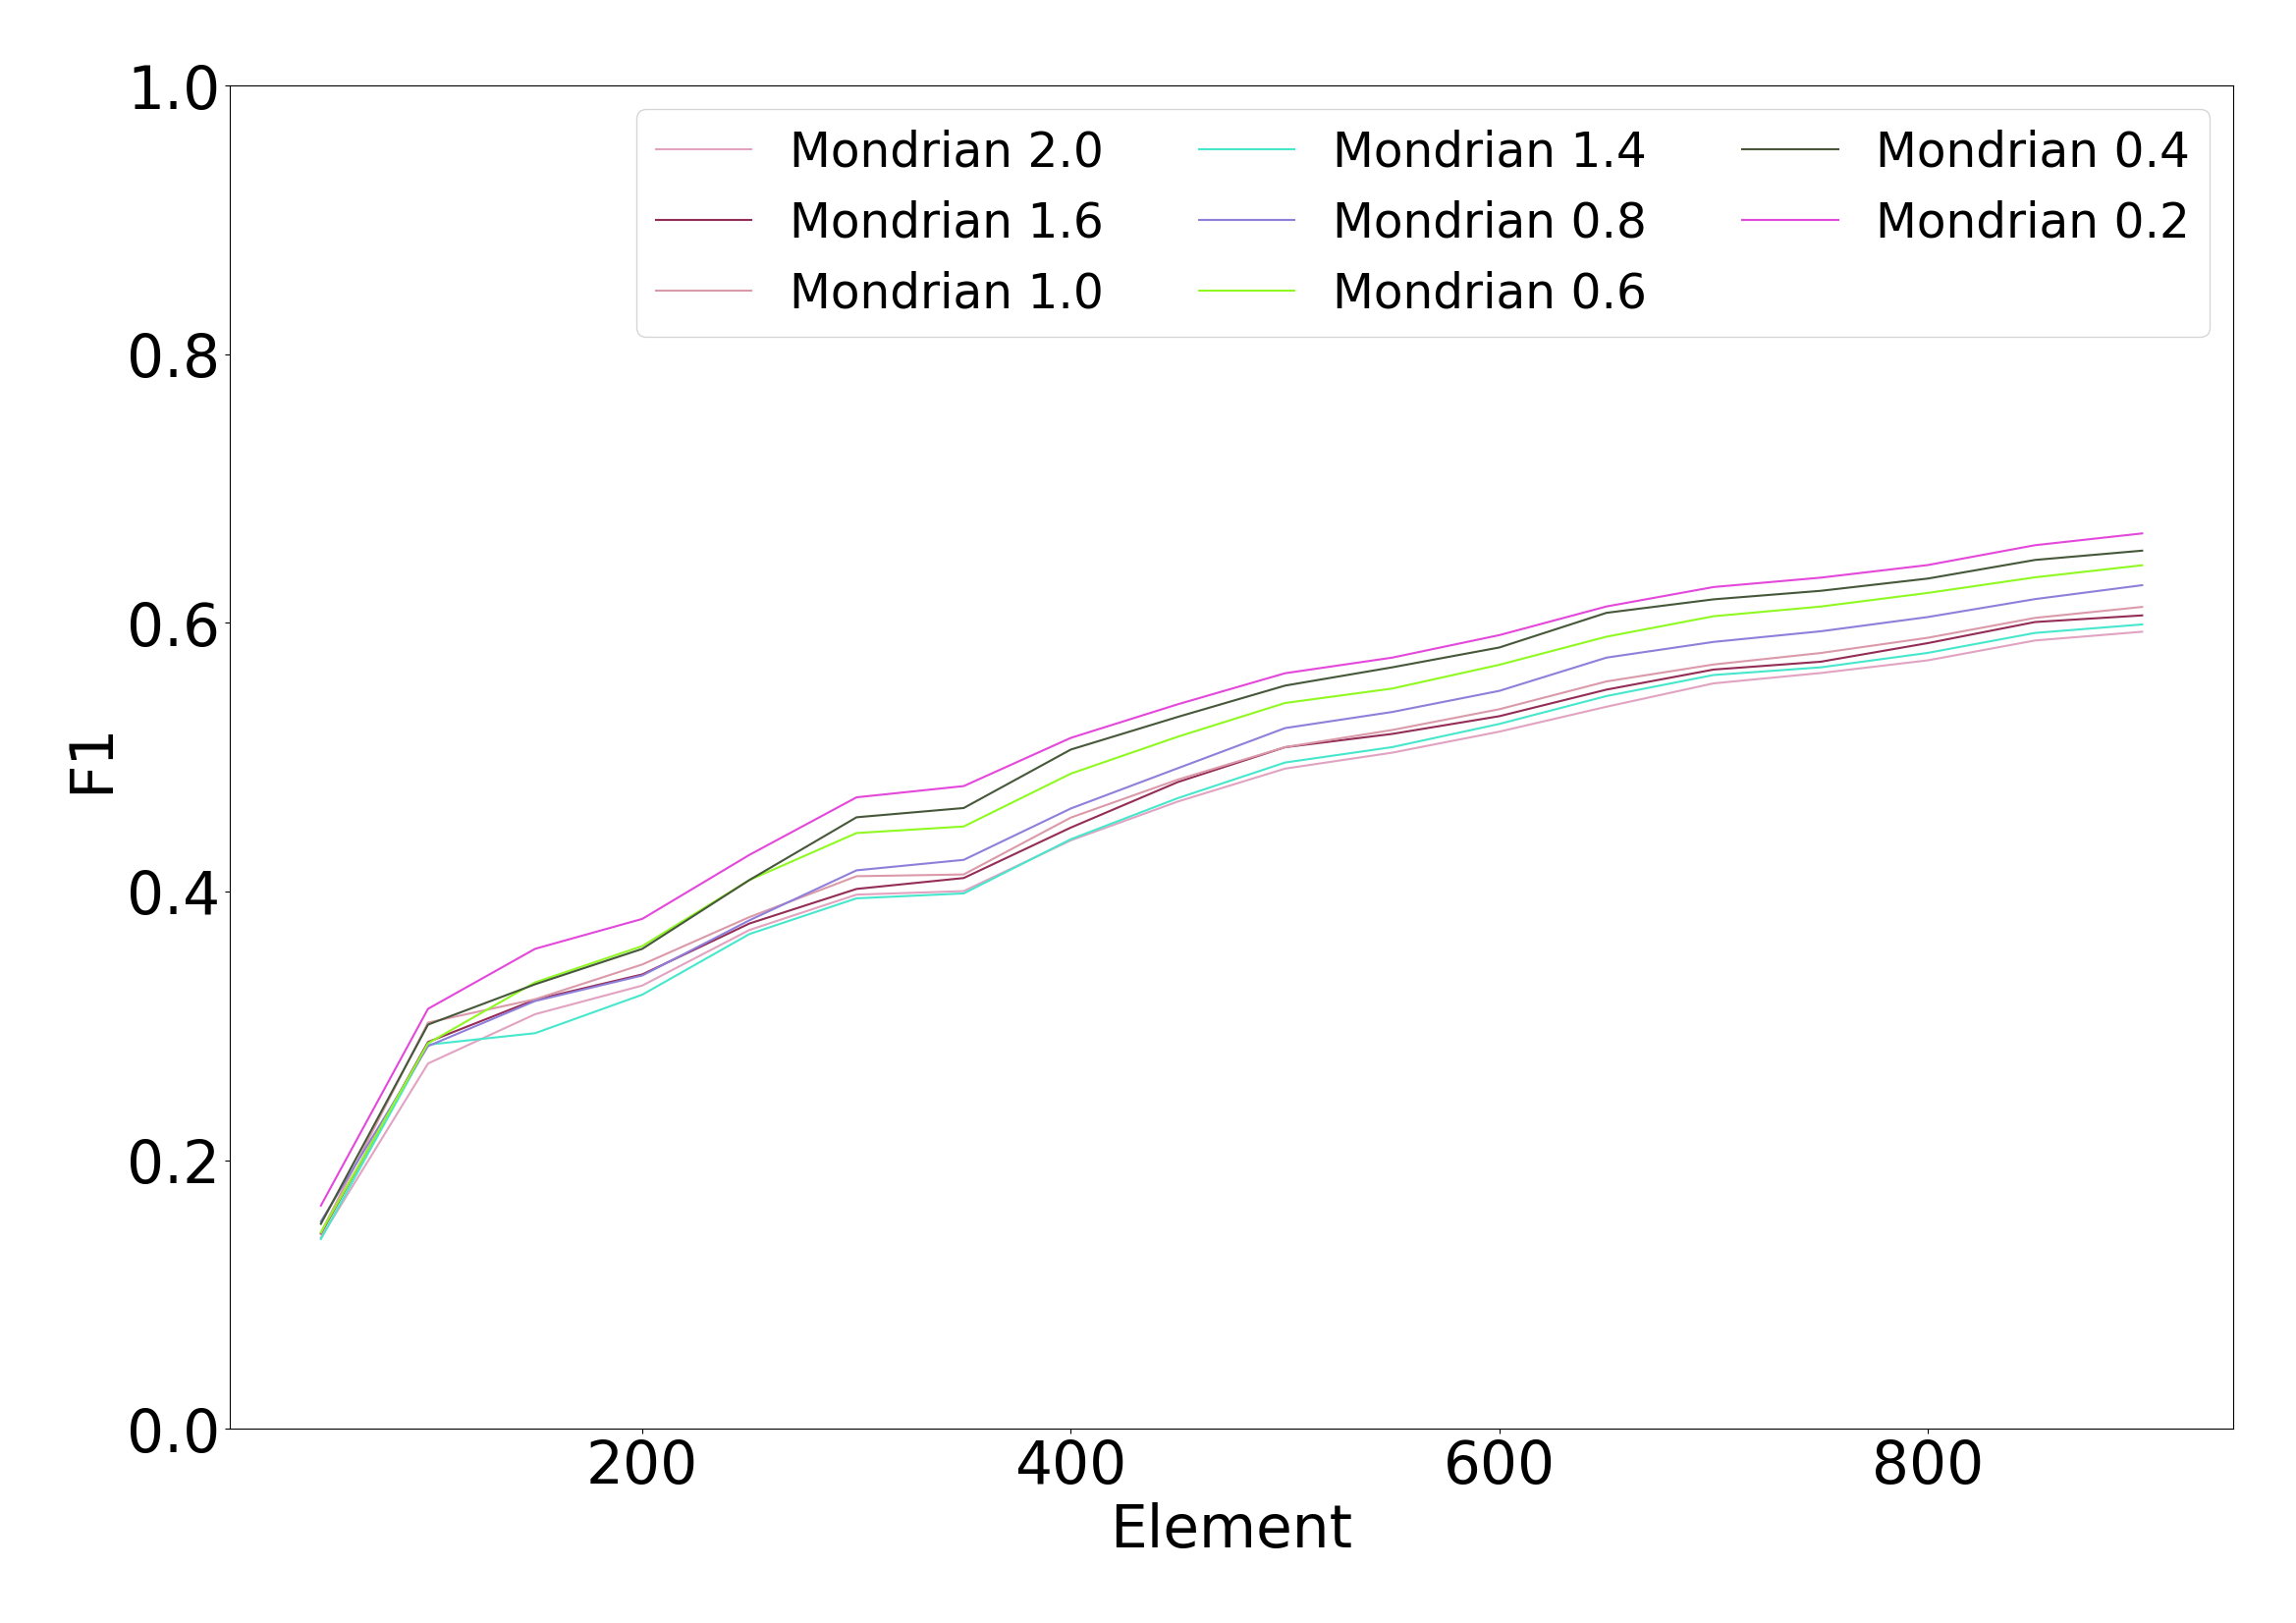
\includegraphics[width=\textwidth]{figures/calibration_mondrian_lifetime.png}
		 \caption{Impact of the budget with 10 trees, a base count of $0.1$, and discount factor of $0.2$.}
		 \label{fig:mondrian-budget}
	 \end{subfigure}
	 \hfill
	 \begin{subfigure}[b]{0.49\textwidth}
		 \centering
		 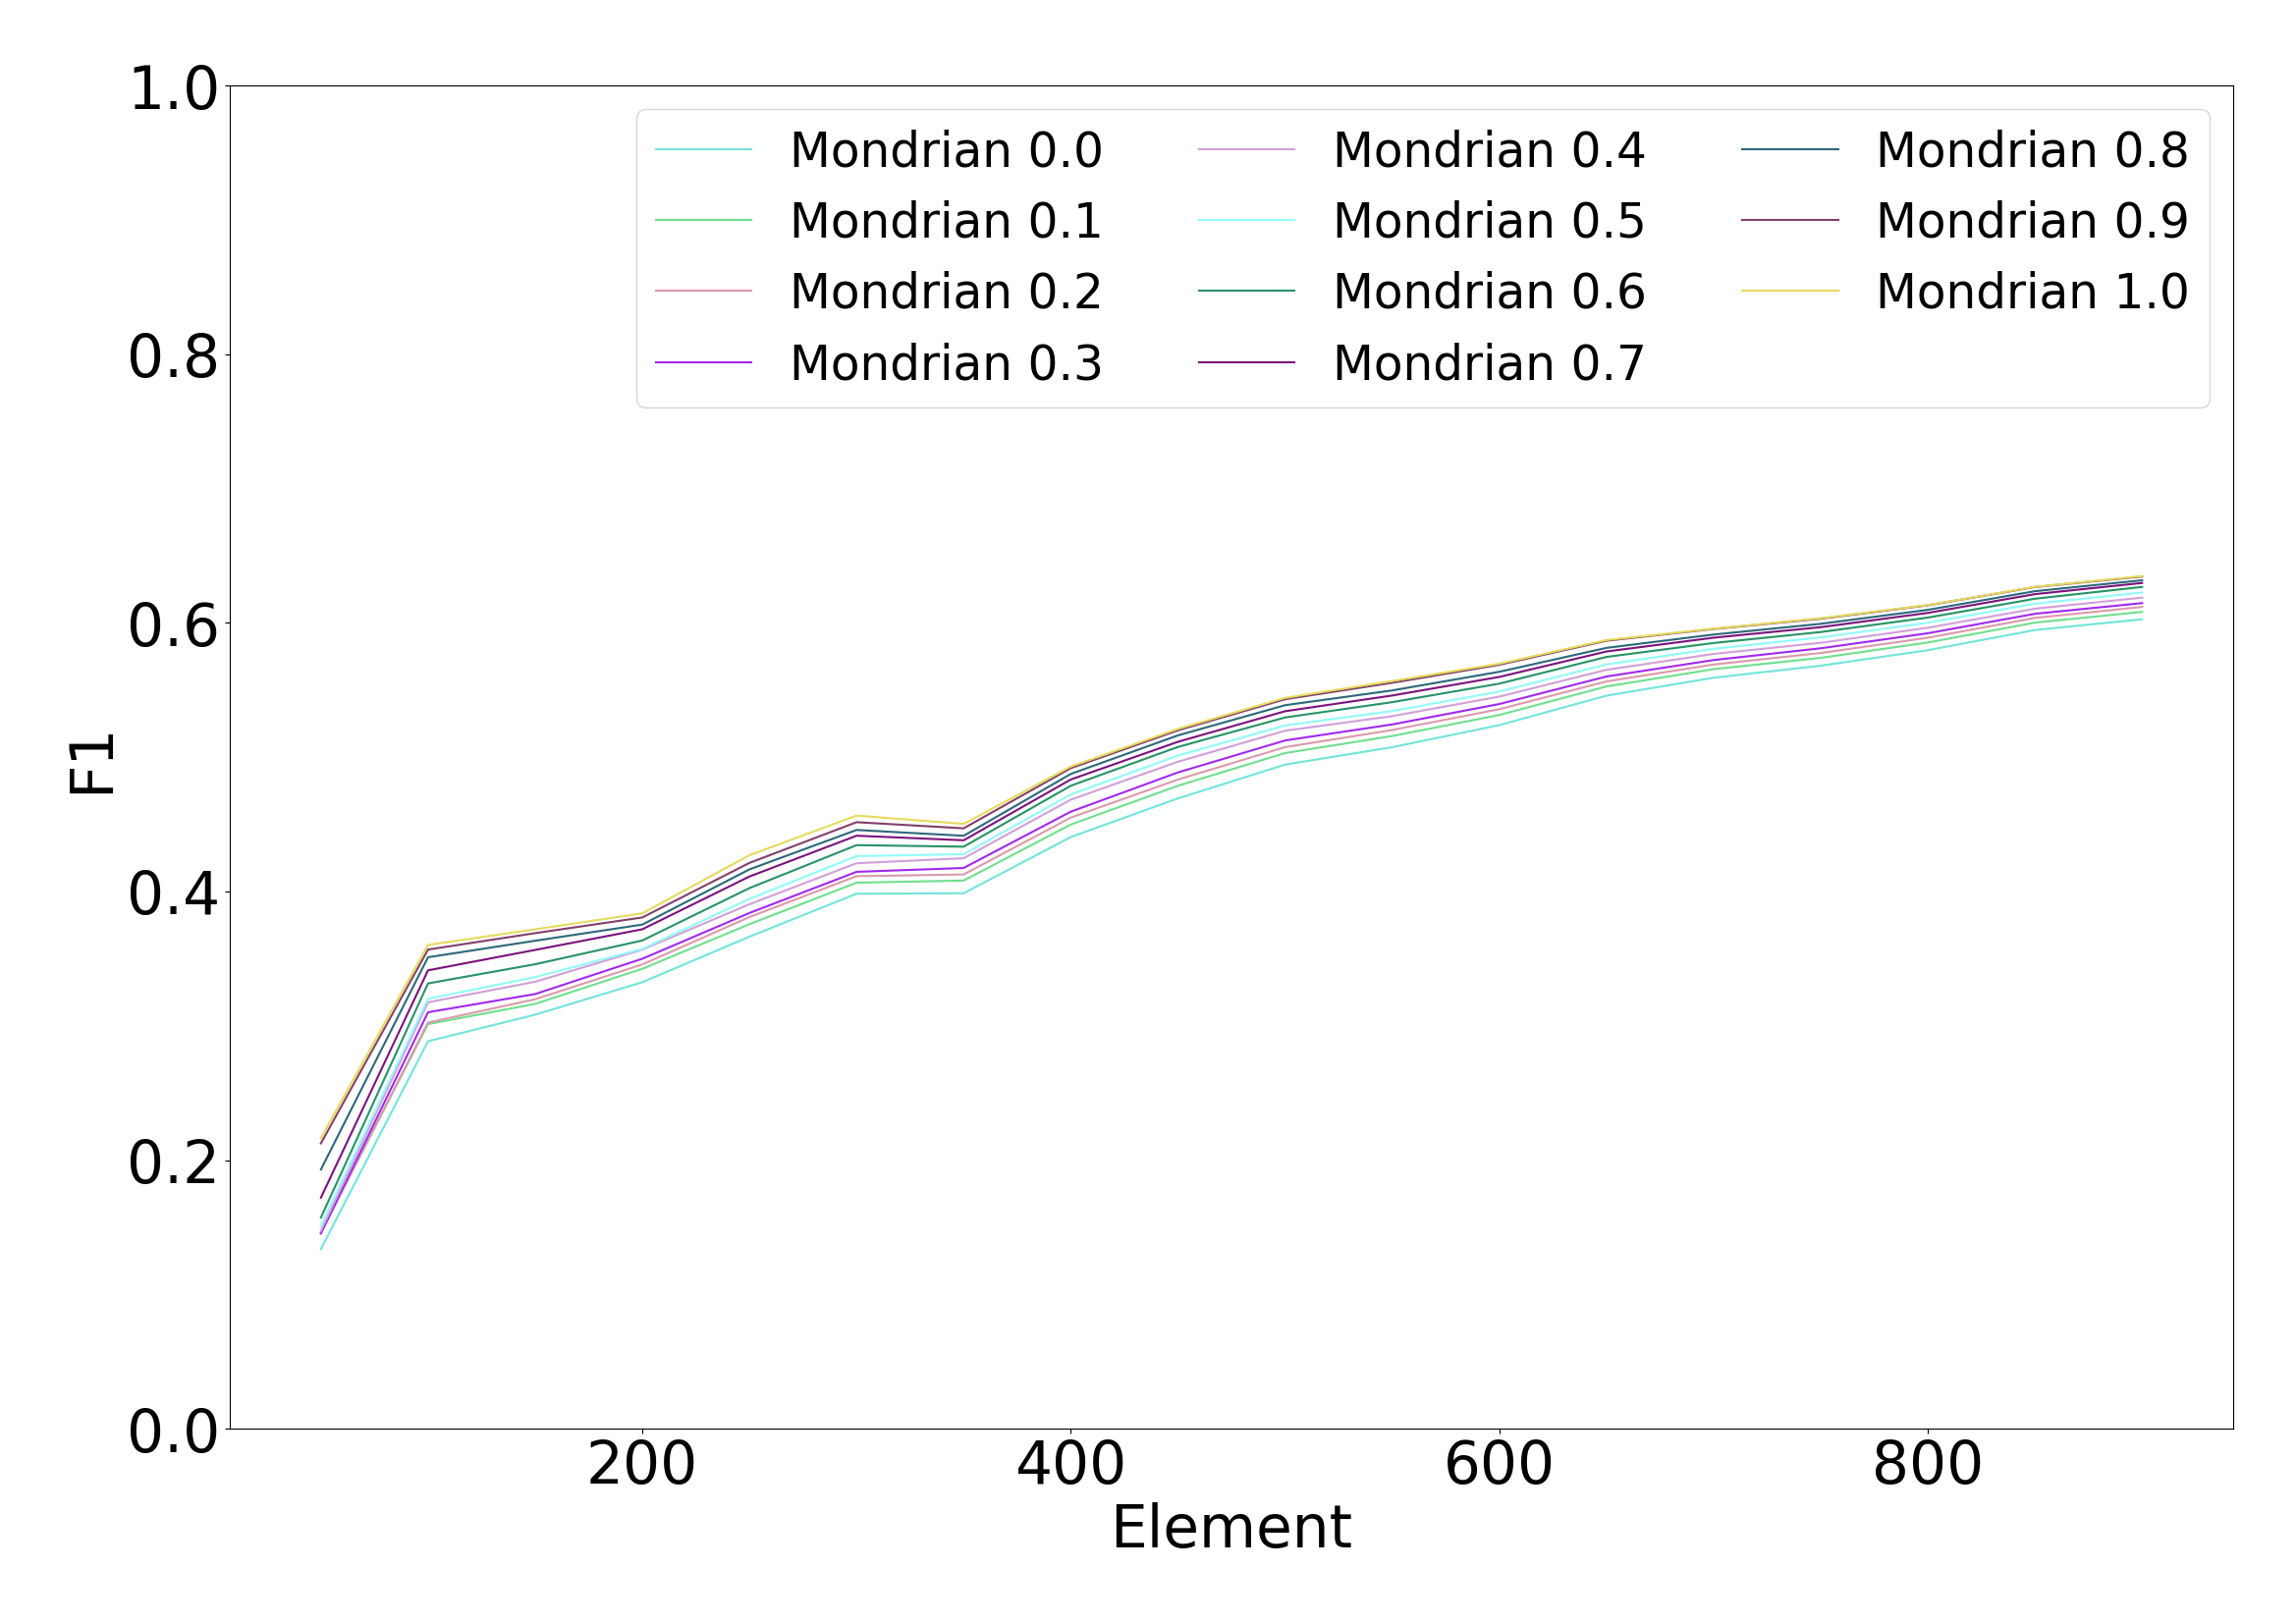
\includegraphics[width=\textwidth]{figures/calibration_mondrian_discount.png}
		 \caption{Impact of the discount factor with 10 trees, a budget of $1.0$, and a base count of $0.1$.}
		 \label{fig:mondrian-discount}
	 \end{subfigure}
		\caption{Hyperparameters tuning for Mondrian with first subject of \banosdataset dataset.}
		\label{fig:mondrian-tuning}
\end{figure}


% vim: tw=80 ts=2
